\documentclass[
version=last,
toc=bib,
toc=graduated,
toc=index,
toc=listof,
fontsize=9pt,
parskip=false,
openany]{scrbook}
%\pdfminorversion=4
\usepackage[utf8]{inputenc}
\usepackage[ngerman]{babel}
\usepackage{fontspec}
\usepackage[default]{sourcesanspro}
\setfontfamily\dejavuSansFont{DejaVu Sans Condensed}

\usepackage{ifmtarg}
\usepackage{ifthen}
\usepackage{etoolbox} % \ifstrempty

\usepackage{geometry}
\geometry{%a6paper
  paperwidth=125mm,
  paperheight=168mm,
  portrait,
  top=22mm,
  inner=22mm,
  outer=20mm,
  bottom=25mm,
  headsep=3mm,
  footskip=12mm
}

\usepackage{ragged2e} % nicer typesetting (hyphenation) for non raggedright and raggedleft
\usepackage{lscape}
\setlength{\parskip}{0pt}

\usepackage{relsize}

\clubpenalty=10000 %keine Schusterjungen
\widowpenalty=10000 
\displaywidowpenalty=10000 % keine Hurenkinder

\usepackage[]{microtype}

\usepackage{graphicx} % graphics

% search path for images
\graphicspath{{images-print/}{icons/}}
\usepackage{wrapfig}  % sponsor logos wrapped with text

\usepackage{tabu}
\usepackage{tabularx}
\usepackage{longtable}
\usepackage[table,cymk]{xcolor}
\usepackage{colortbl}

% embed PDF pages
% pdfpages must not be loaded before colortbl!
\usepackage{pdfpages}
% TikZ must not be loaded before colortbl
\usepackage{tikz}
\usetikzlibrary{calc}

% PDFs als Hintergrundbilder
\usepackage{multirow}
\usepackage{booktabs}
\usepackage{array}
\usepackage{varwidth}

\usepackage{refcount} % calculation of the page where the map is located
\usepackage{svg}
\usepackage{subfigure}

%\DeclareUnicodeCharacter{2032}{minutenstrich}

% page background
\usepackage[manualmark]{scrlayer-scrpage}
\pagestyle{scrplain}

\newcommand{\acro}[1]{{\textsmaller[0.5]{#1}}} % macro for abbreviations with more than one capitalised letter
\newcommand{\keeptabcolsep}{%
  \edef\restoretabcolsep{%
    \tabcolsep=\the\tabcolsep
  }%
}
\newcommand{\demotabcolsep}{%
  \setlength{\tabcolsep}{0.1em}
}%
% title/metadata
%\title{FOSSGIS-Konferenz 2023}
%\subtitle{Programm}
%\author{FOSSGIS e.V.}
%\date{\today}

\clearscrheadings

% page numbers
\cfoot[\begin{small}\pagemark\end{small}]{\begin{small}\pagemark\end{small}}
\ofoot[]{}
\ifoot[]{}
\pagestyle{scrplain}

% Durchschuss erhöhen
\linespread{1.15}

\begin{document}

% include our custom macros
% command for a new time slot
\newcommand{\talkTime}{9:99}
\newcommand{\newTimeslot}[1]{\newpage\renewcommand{\talkTime}{#1}}

% new time slot but without a pagebreak
\newcommand{\newSmallTimeslot}[1]{\renewcommand{\talkTime}{#1}}

% new time slot for Lightning Talk
\newcommand{\newLightningTimeslot}[1]{\renewcommand{\talkTime}{#1 (LT)}}

% initialise \conferenceDay 
\newcommand{\conferenceDay}{Noday}


\input{wallpaper/day-layers.tex}

% define page style for cutting marks without anything else
\DeclareNewLayer[background, oddorevenpage, width=125mm,%
height=169mm, contents={%
  \begin{tikzpicture}[x=1mm, y=1mm]
    \drawCropMarks
  \end{tikzpicture}
}]{cropmarksplain}

% define default page style (cutting marks with page number)
\DeclareNewLayer[background, oddorevenpage, width=125mm,%
height=169mm, contents={%
  \begin{tikzpicture}[x=1mm, y=1mm]
    \drawCropMarks
  \end{tikzpicture}
}]{cropmarksevery}
\newpairofpagestyles[scrheadings]{cropmarksstyle}{}
\AddLayersAtBeginOfPageStyle{cropmarksstyle}{cropmarksevery}

% page style for title pages
\DeclareNewLayer[background, oddorevenpage, width=125mm,%
height=169mm, contents={%
  \includegraphics{wallpaper/front-cover-with-crop-marks.pdf}%
}]{titlelayer}
\newpairofpagestyles[]{titlestyle}{}
\AddLayersAtBeginOfPageStyle{titlestyle}{titlelayer}

% define alias commands for all three days
\def\mittwoch{Mittwoch}
\def\donnerstag{Donnerstag}
\def\freitag{Freitag}
\def\samstag{Samstag}

% define Mittwoch page style
\newpairofpagestyles[scrheadings]{mittwoch-table}{}
\AddLayersAtBeginOfPageStyle{mittwoch-table}{mittwocheven}
\AddLayersAtBeginOfPageStyle{mittwoch-table}{mittwochoddrotated}
\newpairofpagestyles[scrheadings]{mittwoch}{}
\AddLayersAtBeginOfPageStyle{mittwoch}{mittwocheven}
\AddLayersAtBeginOfPageStyle{mittwoch}{mittwochodd}

% define Donnerstag page style
\newpairofpagestyles[scrheadings]{donnerstag-table}{}
\AddLayersAtBeginOfPageStyle{donnerstag-table}{donnerstageven}
\AddLayersAtBeginOfPageStyle{donnerstag-table}{donnerstagoddrotated}
\newpairofpagestyles[scrheadings]{donnerstag}{}
\AddLayersAtBeginOfPageStyle{donnerstag}{donnerstageven}
\AddLayersAtBeginOfPageStyle{donnerstag}{donnerstagodd}

% define Freitag page style
\newpairofpagestyles[scrheadings]{freitag-table}{}
\AddLayersAtBeginOfPageStyle{freitag-table}{freitageven}
\AddLayersAtBeginOfPageStyle{freitag-table}{freitagoddrotated}
\newpairofpagestyles[scrheadings]{freitag}{}
\AddLayersAtBeginOfPageStyle{freitag}{freitageven}
\AddLayersAtBeginOfPageStyle{freitag}{freitagodd}

% define Samstag page style
\newpairofpagestyles[scrheadings]{samstag-table}{}
\AddLayersAtBeginOfPageStyle{samstag-table}{samstageven}
\AddLayersAtBeginOfPageStyle{samstag-table}{samstagoddrotated}
\newpairofpagestyles[scrheadings]{samstag}{}
\AddLayersAtBeginOfPageStyle{samstag}{samstageven}
\AddLayersAtBeginOfPageStyle{samstag}{samstagodd}

% \setpagebackground selects the page style to be used depending on the current day. Each day has
% its own page style.
\newcommand{\setPageBackground}{%
  \ifthenelse{\equal{\conferenceDay}{\mittwoch}}{%
    \pagestyle{mittwoch}%
  }{}%
  \ifthenelse{\equal{\conferenceDay}{\donnerstag}}{%
    \pagestyle{donnerstag}%
  }{}%
  \ifthenelse{\equal{\conferenceDay}{\freitag}}{%
    \pagestyle{freitag}%
  }{}%
  \ifthenelse{\equal{\conferenceDay}{\samstag}}{%
    \pagestyle{samstag}%
  }{}%
}


% additional column type for tables
\newcolumntype{Y}[1]{>{\RaggedRight\arraybackslash}p{#1}}

%% length of the title boxes
\newlength{\titleboxwidth}
\setlength{\titleboxwidth}{\textwidth}
\advance\titleboxwidth by -6pt

\newlength{\roomWidth}
\newlength{\timeWidth}
\newlength{\roomTimeWidth}
\newlength{\titleWidth}
\newcommand{\tmpRoomTimeWidth}{}
\newcommand{\tmpTitleWidth}{}

\DeclareRobustCommand*{\setAbstract}[6]{%
  % 1. speaker
  % 2. title
  % 3. subtitle
  % 4. abstract (Text)
  % 5. colour
  % 6. room
  \setPageBackground%
  \calculateRoomTimeAndTitleWidth{#1}{#6}%
  \noindent\fcolorbox{white}{#5}{%
    \noindent\parbox{\titleboxwidth}{%
      \isSpeakerEmpty{#1}{#2}{#6}%
      \isSubtitleEmpty{#3}%
    }%
  }%
  %
  \justifying
  \isAbstractEmpty{#4}%
  \vspace{0.5em}% space to the next talk even if there is no abstract
}

% Calculate width of title and room/time field
% Arguments: speaker, room
\makeatletter
  \newcommand{\calculateRoomTimeAndTitleWidth}[2]{%
    \@ifmtarg{#1}{% speaker is empty
      \settowidth{\roomWidth}{#2, \talkTime}%
    }{% speaker is not empty
      \settowidth{\roomWidth}{#2}%
    }%
    \settowidth{\timeWidth}{\talkTime}%
    \directlua{require("lua/titleWidth")}%
    \setlength{\titleboxwidth}{\directlua{getTitleBoxWidth()}}%
    \renewcommand{\tmpRoomTimeWidth}{\directlua{getTimeRoomWidth()}}%
    \setlength{\roomTimeWidth}{\tmpRoomTimeWidth}%
    \renewcommand{\tmpTitleWidth}{\directlua{getTitleWidth()}}%
    \setlength{\titleWidth}{\tmpTitleWidth}%
  }%
\makeatother

% Lay out the subtitle
% has to be a separate function and has to be surrounded by \makeatletter for technical reasons
\makeatletter
  \newcommand{\isSubtitleEmpty}[1]{%
    \@ifnotmtarg{#1}{%
      \par
      \RaggedRight
      \vspace{0.3\baselineskip}
      \noindent%
      \bfseries%
      #1%
    }
  }
\makeatother

% lay out the speaker if there is any
% We assume that there is only a subtitle if the talk has a speaker.
\makeatletter
  \newcommand{\isSpeakerEmpty}[3]{%
    % Arguments:
    % 1. speaker
    % 2. title
    % 3. room
    \@ifmtarg{#1}{%
      \begin{minipage}[t][][t]{\titleWidth}
        \RaggedRight
        \noindent%
        {\large \sectfont #2}%
      \end{minipage}%
      \hfill
      \begin{minipage}[t][][t]{\roomTimeWidth}
        \RaggedLeft%
        \noindent #3, \talkTime%
      \end{minipage}%
    }%
    {%
      \begin{minipage}[t][][t]{\titleWidth}
        \RaggedRight
        \noindent
        \emph{#1} % speaker
        \par%
        \noindent%
        {\large \sectfont #2}%
      \end{minipage}%
      \hfill
      \begin{minipage}[t][][t]{\roomTimeWidth}
        \RaggedLeft
        \noindent
        \talkTime%
        \par%
        \noindent #3% room
      \end{minipage}%
    }%
  }
\makeatother

% Lay out the abstract if there is any
% has to be a separate function and has to be surrounded by \makeatletter for technical reasons
\makeatletter
\newcommand{\isAbstractEmpty}[1]{%
  \ifstrempty{#1}{%
    \vspace{1.5em}%
  }{%
    \vspace{0.5em}\newline%
    #1 \par% % abstract
    \vspace{1.5em}% space to the next talk even if there is an abstract
  }%
}
\makeatother

% define colours
%\definecolor{eins}{cmyk}{0 .18 .06 .10}
\definecolor{eins}{cmyk}{0 .13 .04 .08}
\definecolor{zwei}{cmyk}{.1 0 .17 .05}
\definecolor{hellorange}{cmyk}{0 0.18 0.40 0.03}
\definecolor{audimax}{cmyk}{0.13 0 0.04 0.11}
\definecolor{geoblau}{cmyk}{0.24 .02 0 .01}
\definecolor{dezentrot}{cmyk}{0 .24 0.29 .04}
\definecolor{hellgelb}{cmyk}{0 .02 0.36 0}
\definecolor{hellgruen}{cmyk}{0.10 .0 0.22 0.05}

% abstract at HS 1
\DeclareRobustCommand*{\abstractHSeins}[4]%
{%
  \setAbstract{#1}{#2}{#3}{#4}{geoblau}{HS 1 (Audimax 1)}
}

% abstract at HS 2
\DeclareRobustCommand*{\abstractHSzwei}[4]%
{%
  \setAbstract{#1}{#2}{#3}{#4}{hellgelb}{HS 2 (Ditze H016)}
}

% abstract at HS 3
\DeclareRobustCommand*{\abstractHSdrei}[4]%
{%
  \setAbstract{#1}{#2}{#3}{#4}{hellgruen}{HS 3 (K0506/Audi 2)}
}

% abstract at HS 4
\DeclareRobustCommand*{\abstractHSvier}[4]%
{%
  \setAbstract{#1}{#2}{#3}{#4}{dezentrot}{HS 4 (A.013)}
}

% abstract at Expert:innen (H.04)
\DeclareRobustCommand*{\abstractExp}[4]%
{%
  \setAbstract{#1}{#2}{#3}{#4}{audimax}{Expert. (H.04)}

}
% abstract at Anwendertreffen | BoF1 (H.09)
\DeclareRobustCommand*{\abstractAnwBoFeins}[4]%
{%
  \setAbstract{#1}{#2}{#3}{#4}{eins}{Anw./BoF1 (H.09)}
}

% abstract at Anwendertreffen | BoF2 (H.08)
\DeclareRobustCommand*{\abstractAnwBoFzwei}[4]%
{%
  \setAbstract{#1}{#2}{#3}{#4}{zwei}{Anw./BoF2 (H.08)}
}

% abstract at a different location
\newcommand{\abstractOther}[5]%
{%
  \setAbstract{#1}{#2}{#3}{#4}{hellorange}{#5}
}

% infobox for workshops (they don't have an abstract in the booklet)
\newcommand{\workshopbox}[3]{%
  % 1. titel
  % 2. speaker
  % 3. Room
  \setlength\tabcolsep{2pt}%
  \noindent\fcolorbox{white}{dezentrot}{%
    \parbox{\titleboxwidth}{%
      \noindent%
      \begin{tabu}{X[5L]r}
        \emph{#2} % Sprecher
        &
        \talkTime
        \tabularnewline
        {\noindent\large \bfseries #1}% % title
        &
        #3
        \tabularnewline
      \end{tabu}
    }
  }
  \setlength\tabcolsep{6pt} % set column padding back to default
}

% too long
\newcommand{\tooLong}{Dieser Text ist viel zu lang. Dieser Text ist viel zu lang. Dieser Text ist viel zu lang. Dieser Text ist viel zu lang. Dieser Text ist viel zu lang. Dieser Text ist viel zu lang. Dieser Text ist viel zu lang. Dieser Text ist viel zu lang. Dieser Text ist viel zu lang. Dieser Text ist viel zu lang. Dieser Text ist viel zu lang. Dieser Text ist viel zu lang. Dieser Text ist viel zu lang. Dieser Text ist viel zu lang. }

\newlength{\fboxwidth}

\def\workshopsSection{workshopsSection}
\def\abstractsSection{abstractsSection}

% boxes for text-only advertisement texts by our sponsors
\newcommand{\sponsorBox}[4]{%
  \setlength{\fboxwidth}{\textwidth}
  \advance\fboxwidth by -7.0pt
  \abstractSponsorbox{#1}{#2}{#3}{#4}{\workshopsSection}%
}

\newcommand{\sponsorBoxA}[4]{%
  \setlength{\fboxwidth}{\textwidth}%
  \advance\fboxwidth by -10.0pt%
  \abstractSponsorbox{#1}{#2}{#3}{#4}{\abstractsSection}%
}

\newcommand{\sponsorBoxLandscape}[4]{%
  \setlength{\fboxwidth}{\linewidth}
  \advance\fboxwidth by -10.0pt
  \abstractSponsorbox{#1}{#2}{#3}{#4}{\abstractsSection}%
}

%% store \parindent in separate variable because it is resetted to 0 in parboxes
\newlength{\saveparindent}
\setlength{\saveparindent}{\parindent}

%% box for advertisment by a sponsor
%% 1. logo (leave empty if none)
%% 2. width of the logo (leave empty if none
%% 3. number of required lines of the logo (due to usage of wrapfigure)
%% 4. text
%% 5. where we are in the booklet (\workshopsSection or \abstractsSection}
\makeatletter
  \newcommand{\abstractSponsorbox}[5]{%
    \setlength{\fboxsep}{4.5pt}%
    \noindent%
    \ifthenelse{\equal{#5}{\workshopsSection}}{%
      \hspace{2.65pt}%
    }{%
      \hspace{-1pt}%
    }%
    \fcolorbox{gray}{white}{%
      \parbox{\fboxwidth}{%
        \setlength{\parindent}{\saveparindent}%
        \@ifmtarg{#1}{}{%
          \begin{wrapfigure}[#3]{r}[0pt]{#2}%
            \centering\vspace{-1\baselineskip}%
            \includegraphics[width=#2]{#1}%
          \end{wrapfigure}%
        }%

        \noindent #4
      }%
    }%
    \setlength{\fboxsep}{3pt}%
  }%
  \setlength{\fboxsep}{3pt}%
\makeatother

% definition of column types for the schedule tables
\newcolumntype{Z}[1]{>{\RaggedRight\arraybackslash}p{#1}}%
\newcolumntype{C}[1]{>{\Centering\arraybackslash}p{#1}}%

% common implementation of typesetting of a session in the tables
\newcommand{\talkInternal}[2]{%
  \textbf{#1}
  \ifthenelse{\equal{#2}{}}{}{%
    \newline\emph{#2}%
  }
}

% common implementation of typesetting of a session in the tables -- singleline mode
\newcommand{\talkInternalSingleLine}[2]{%
  \textbf{#1}
  \hspace{0.5em}
  \ifthenelse{\equal{#2}{}}{}{%
    \emph{#2}%
  }
}

% macro to typeset a talk in the schedule tables spanning over more than one row:
% usage: \longTalk{rowcount}{title}{speaker}
\newcommand{\longTalk}[3]{%
  &
  \multirow{#1}{\linewidth}{%
    \parbox{\linewidth}{
      %HACK Inserting a \vspace here is a dirty hack but it works.
      \vspace{0.45\baselineskip}
      \talkInternal{#2}{#3}%
    }
  }%
}%

% macro to typeset a talk in the schedule tables:
% usage: \talk{title}{speaker}
\newcommand{\talk}[2]{%
  &
  \talkInternal{#1}{#2}%
}%

% macro to typeset a talk in the schedule tables, single line mode:
% usage: \talkSingleLine{title}{speaker}
\newcommand{\talkSingleLine}[2]{%
  &
  \talkInternalSingleLine{#1}{#2}%
}%


% macro to typeset a talk in the schedule tables spanning over more than one column:
% usage: \multiColTalk{columns}{columnSpecs}{title}{speaker}
\newcommand{\multiColTalk}[4]{%
  &
  \multicolumn{#1}{#2}{\talkInternal{#3}{#4}}%
}%

% set time in scheduel table
\newcommand{\tableRowFirstCell}[1]{%
  \cellcolor{table-header}
  \textcolor{black}{#1}%
}

% set time in scheduel table
\newcommand{\tableColHead}[1]{%
  \cellcolor{table-header}%
  \textcolor{black}{#1}%
}

\newcommand{\workshop}[3]%
{%
  \workshopbox{#1}{#2}{#3}%
}%

\newcommand{\otherevent}[1]%
{%
  & \textbf{#1}
}%

\newcommand{\audimaxEvent}[2]%
{%
  &
  \multicolumn{3}{c}{
    \textbf{#1} (Audimax) \par \emph{#2}
  }
}%

\newcommand{\coffeespace}{\vspace{0.4em}}
\newcommand{\workshopspace}{\vspace{0.5em}\\}

% define colors
\definecolor{commongray}{gray}{.9}
\definecolor{tableRuleGray}{gray}{.9}
\definecolor{textGray}{gray}{.45}

% macro for table rules
\newcommand{\programCRule}[1]{%
  \cline{#1}%
}
\newcommand{\programHRule}[1]{%
  \cline{2-#1}%
}

% macro for empty session slots
\newcommand{\bookableSpace}{
  & \emph{\textcolor{textGray}{Bookable Space}}%
}

% diamond symbol for shortened titles
\newcommand{\diamondSymbol}{%
  \textsuperscript{%
    \diamond%
  }%
}

% speaker affiliation
\newcommand{\speakerAffiliation}[1]{%
  (#1)%
}

% lightning talk (title and author)
\newcommand{\lightningTalk}[2]{%
  \item \emph{#2:} #1%
}

% macro for no-video icon
\newcommand{\noVideo}{%
  \raisebox{-0.2\height}{%
    \includegraphics[height=8pt]{novideo.pdf}%
  }%
}

% Titelseite
\DeclareNewLayer[background,%
%  width=115mm,%
 % height=158mm,%
% hoffset=5mm,%
% voffset=5mm,%
  width=115mm,%
  height=158mm,%
  hoffset=10mm,%
  voffset=10mm,%
  contents={%
   \begin{tikzpicture}[x=1mm, y=1mm]%
      % map image
      \draw (0,0) node [inner sep=0mm, anchor=south west] {%
        \includegraphics[height=148mm]{images-print/Entwurf_Titelbild_A6_mDatum.png}%
      };%
      \end{tikzpicture}%
   }%
]{titelseite}
\newpairofpagestyles[]{page-title}{}
\AddLayersAtBeginOfPageStyle{page-title}{titelseite}
\AddLayersAtBeginOfPageStyle{page-title}{cropmarksplain}

% Übersicht alle Häuser 
\DeclareNewLayer[background,%
  width=115mm,%
  height=158mm,%
  hoffset=10mm,%
  voffset=10mm,%
  contents={%
    \begin{tikzpicture}[x=1mm, y=1mm]%
      % map image
      \draw (0,0) node [inner sep=0mm, anchor=south west] {%
        \includegraphics[height=148mm]{images-print/A6_Häuser_V2.pdf}%
      };%
      \end{tikzpicture}%
   }%
]{uebersicht-alle-haeuser}
\newpairofpagestyles[]{page-uebersicht-alle-haeuser}{}
\AddLayersAtBeginOfPageStyle{page-uebersicht-alle-haeuser}{uebersicht-alle-haeuser}
\AddLayersAtBeginOfPageStyle{page-uebersicht-alle-haeuser}{cropmarksplain}

% Haus A+D
\DeclareNewLayer[background,%
  width=115mm,%
  height=158mm,%
  hoffset=10mm,%
  voffset=10mm,%
  contents={%
    \begin{tikzpicture}[x=1mm, y=1mm]%
      % map image
      \draw (0,0) node [inner sep=0mm, anchor=south west] {%
        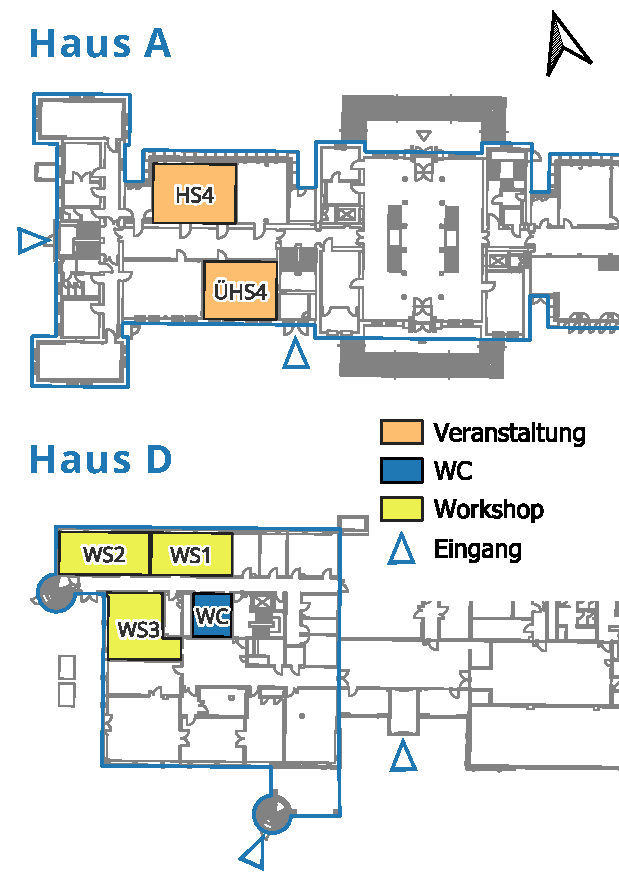
\includegraphics[height=148mm]{images-print/A6_Haus_A_+_D_V2.pdf}%
      };%
      \end{tikzpicture}%
   }%
]{Haus_A+D}
\newpairofpagestyles[]{page-Haus_A+D}{}
\AddLayersAtBeginOfPageStyle{page-Haus_A+D}{Haus_A+D}
\AddLayersAtBeginOfPageStyle{page-Haus_A+D}{cropmarksplain}

% Haus H (EG + OG)
\DeclareNewLayer[background,%
  width=115mm,%
  height=158mm,%
  hoffset=10mm,%
  voffset=10mm,%
  contents={%
    \begin{tikzpicture}[x=1mm, y=1mm]%
      % map image
      \draw (0,0) node [inner sep=0mm, anchor=south west] {%
        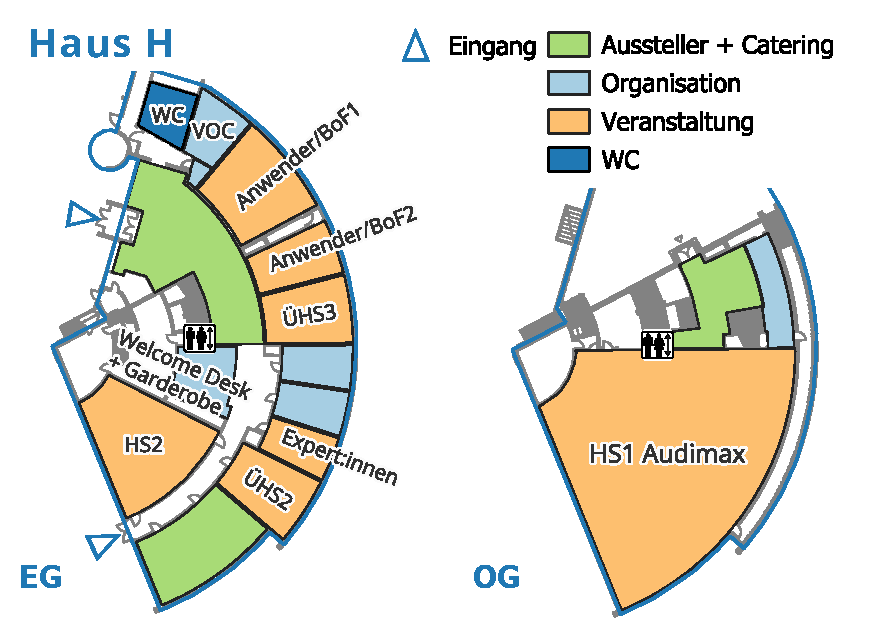
\includegraphics[width=148mm,angle=90,origin=c]{images-print/A6_Haus_H_V2.pdf}%
      };%
      \end{tikzpicture}%
   }%
]{Haus_H_EG_+_OG}
\newpairofpagestyles[]{page-Haus_H_EG_+_OG}{}
\AddLayersAtBeginOfPageStyle{page-Haus_H_EG_+_OG}{Haus_H_EG_+_OG}
\AddLayersAtBeginOfPageStyle{page-Haus_H_EG_+_OG}{cropmarksplain}

% Haus K+I
\DeclareNewLayer[background,%
  width=115mm,%
  height=158mm,%
  hoffset=10mm,%
  voffset=10mm,%
  contents={%
    \begin{tikzpicture}[x=1mm, y=1mm]%
      % map image
      \draw (0,0) node [inner sep=0mm, anchor=south west] {%
        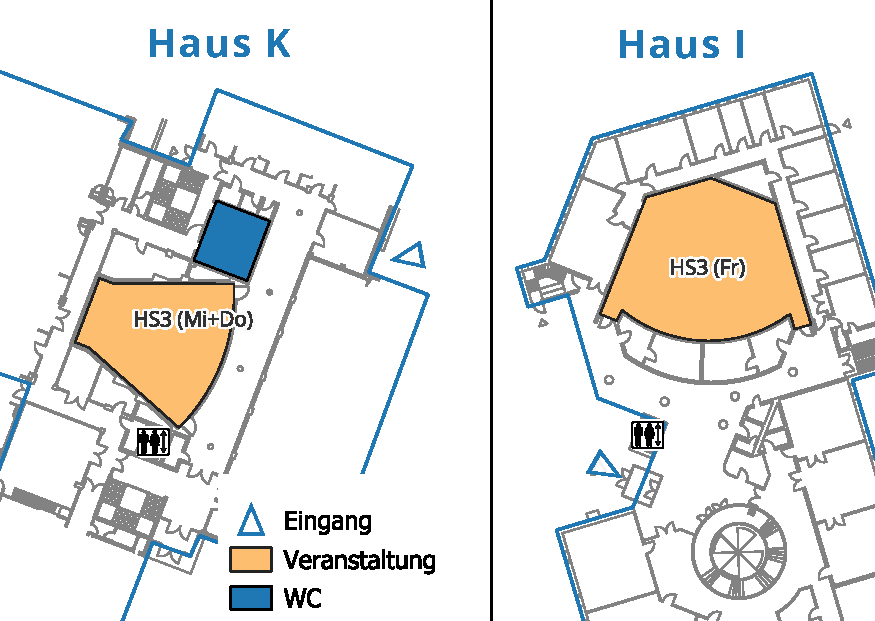
\includegraphics[width=148mm,angle=90,origin=c]{images-print/A6_Haus_K+I_V2.pdf}%
      };%
      \end{tikzpicture}%
   }%
]{Haus_K+I}
\newpairofpagestyles[]{page-Haus_K+I}{}
\AddLayersAtBeginOfPageStyle{page-Haus_K+I}{Haus_K+I}
\AddLayersAtBeginOfPageStyle{page-Haus_K+I}{cropmarksplain}


 
\pagestyle{cropmarksstyle}
\begin{titlepage}
  \thispagestyle{page-title}
  \null
\end{titlepage}
\pagestyle{cropmarksstyle}

\pagenumbering{gobble}\section*{Notizen}

\newpage
\pagenumbering{arabic}
%\setcounter{page}{1}
\section*{Inhalt}
\label{contents}
\newlength\contentspace
\setlength\contentspace{0.2em}

\vspace*{\contentspace}%
\noindent Abendveranstaltung, Exkursionen, Rahmenprogramm  \dotfill \pageref{schwaetzli}

\vspace*{\contentspace}%
\noindent Platin- und Goldsponsoren \dotfill \pageref{platinsposoren}

\vspace*{\contentspace}%
\noindent Workshops am Mittwoch \dotfill \pageref{mittwoch-workshops}

\vspace*{\contentspace}%
\noindent Workshops am Donnerstag \dotfill \pageref{donnerstag-workshops}

\vspace*{\contentspace}%
\noindent Workshops am Freitag \dotfill \pageref{freitag-workshops}

\vspace*{\contentspace}%
\noindent Vorträge am Mittwoch \dotfill \pageref{mittwoch}

\vspace*{\contentspace}%
\noindent Vorträge am Donnerstag \dotfill \pageref{donnerstag}

\vspace*{\contentspace}%
\noindent Vorträge am Freitag \dotfill \pageref{freitag}

\vspace*{\contentspace}%
\noindent OpenStreetMap-Samstag \dotfill \pageref{samstag}

\vspace*{\contentspace}%
\noindent Impressum \dotfill \pageref{impressum}

\vspace*{\contentspace}%
\noindent Medienpartner \dotfill \pageref{medienpartner}

\vspace*{\contentspace}%
\noindent Campusplan und Raumpläne \dotfill \pageref{kartenseiten}

\justifying

\newpage

\newpage
\section*{Willkommen zur FOSSGIS-Konferenz 2023 in Berlin!}\label{welcome}
Die Abkürzung { FOSSGIS} steht für {\bfseries f}reie und {\bfseries O}pen"={\bfseries S}ource"={\bfseries S}oftware für {\bfseries G}eo{\bfseries i}nformations{\bfseries s}ysteme.
Die FOSSGIS-Konferenz 2023 wird vom gemeinnützigen FOSSGIS e.V., der
OpenStreetMap"=Community und der Humboldt-Universität zu Berlin
veranstaltet.
Ziel der jährlich stattfindenden Konferenz ist die Verbreitung von freier,
quelloffener Software für Geoinformationssysteme. In den nächsten vier Tagen
haben Sie die Gelegenheit, sich mit Entwickler:innen und anderen Anwender:innen
auszutauschen und \mbox{neueste} Informationen zu Anwendungen und
Arbeitsmöglichkeiten zu erhalten.

\section*{Anwender- und Expert:innentreffen, Birds of a Feather}
Die FOSSGIS-Konferenz ist eine Communityveranstaltung.
Die gesamte Konferenz über stehen zwei Räume für Anwender- und Expert:innentreffen oder spontan organisierte
Treffen Gleichgesinnter (Birds of a Feather), u.\,ä.
zur Verfügung. Eigene Sessions können Sie an der Pinnwand im Foyer selbst eintragen.
\pagebreak

\section*{Abendveranstaltung am Mittwoch}\label{schwaetzli}
Traditionell findet am ersten Abend der FOSSGIS-Konferenz die
Abendveranstaltung statt, auch Social Event genannt. Der Eintritt
ist im FOSSGIS-Konferenz-Ticket enthalten. Eine Anmeldung ist erforderlich.
Die Abendveranstaltung wird am Konferenzstandort im Erwin-Schrödinger-Zentrum
ab {\bfseries 18:30 bis 22:00 Uhr} stattfinden.

\section*{Mapathon mit Ärzte ohne Grenzen am Freitag und Samstag}
Ärzte ohne Grenzen lädt im Rahmen der FOSSGIS Konferenz 2023 zu einem Mapathon ein. Die Initiative hat das Ziel die Erstellung und Vervollständigung von Kartenmaterial zu unterstützen, welches die Hilfe für Menschen in Krisengebieten erleichtern kann. Es wird eine Einführung geben. Weitere Informationen sind hier zu finden. FOSSGIS-Teilnehmende sind eingeladen, mitzumachen, auch wenn sie noch nie gemappt haben.
Termine: {\bfseries Freitag, 17.00 bis 20.00 Uhr} und {\bfseries Samstag, 11.00 bis 14.00 Uhr}. Bitte melden Sie sich über den Anmeldelink auf der Konferenzwebseite an.
\pagebreak

\section*{Exkursionen}
\subsection*{Kartenabteilung der Staatsbibliothek zu Berlin}
Von den Sektionskarten von Balbi und der Preußischen Uraufnahme zu digitalen Kartendaten.
Am {\bfseries Freitagnachmittag} und {\bfseries Samstagvormittag} werden Führungen durch die Karten\-abteilung der Staatsbibliothek zu Berlin im Haus Unter den Linden angeboten. Anmeldung erforderlich.

\subsection*{Campus Adlershof/WISTA-Gelände}
Die FOSSGIS 2023 findet auf dem Gelände des Wissenschafts- und Wirtschaftsstandort Adlershof (WISTA) statt. Dort existieren noch mehrere technische Denkmale, wie beispielsweise der Trudelturm, die an den Beginn der Luftfahrtindustrie auf dem Campus erinnern. Zu sehen sind aber auch moderne Forschungseinrichtungen, Gründer- und Technologiezentren, die auf die heutige Entwicklung als Zukunftsort für Forschung und Innovation verweisen. In einer kleinen, etwa 60-minütigen Führung können wir sowohl dieser Geschichte als auch den neuen Trends nachstöbern und mehr über den Standort Adlershof erfahren.
Die Exkursion startet am {\bfseries Freitag} um {\bfseries 16:30 Uhr} (nach dem Sektempfang) vor dem Haupteingang des Erwin-Schrödinger-Zentrums. Anmeldung erforderlich.

\section*{Rahmenprogramm am Donnerstag}
\subsection*{Gruppenfoto}
Auch in diesem Jahr wollen wir uns das Gruppenfoto nicht entgehen lassen und laden Sie ein am {\bfseries Donnerstag} in der {\bfseries Nachmittagspause} zum gemeinsamen Gruppenfoto am Haupteingang des Erwin-Schrödinger-Zentrums ein.

\subsection*{Treffen der Freiberufler}
Am {\bfseries Donnerstag} werden sich um {\bfseries 17:45 Uhr} die Freiberufler aus dem FOSSGIS-Bereich im Seminarraum 1\textquotesingle 306 zum gemeinsamen Austausch treffen.

\subsection*{Mitgliederversammlung des FOSSGIS e.\,V.}
Am {\bfseries Donnerstag} sind alle Mitglieder und Gäste ab {\bfseries 18.00 Uhr} herzlich eingeladen, an der Mitgliederversammlung teilzunehmen und sich zu beteiligen. Der FOSSGIS e.\,V. lädt zum Diskutieren, Kennenlernen, Abstimmen und zu Neuwahlen ein. Es wird Getränke und Pizza für alle geben. Der Verein freut sich über zahlreiches Erscheinen.

\section*{Rahmenprogramm am Freitag}
\subsection*{Jeopardy-Quiz}
Am {\bfseries Freitag} gibt es vor dem Abschluss des reguläres Konferenzprogramms um {\bfseries 14.30 Uhr} das nunmehr legendäre und sehr humorvolle Quiz in Form des FOSSGIS-Jeopardy mit Hannes und Tobia.

\subsection*{Sektempfang am FOSSGIS-Stand}
Alle Mitglieder des FOSSGIS-Vereins, Freunde und Interessierte sind am {\bfseries Freitag} ab {\bfseries 16.00 Uhr} herzlich zum Sektempfang zum Ausklang der FOSSGIS 2023 am FOSSGIS-Vereins-Stand eingeladen.

\subsection*{OSM-Event am Freitagabend}
Für alle, die am {\bfseries Freitagabend} noch in der Stadt sind und/oder am OSM-Event teilnehmen möchten gibt es um {\bfseries 19/19:30 Uhr} ein gemeinsames Treffen im Restaurant Greek Food Olympia, Rudower Chaussee 5a in 12489 Berlin-Adlershof. Jeder zahlt seine Rechnung selbst.

\small
\newpage
\label{platinsposoren}
\cleardoubleevenpage
\section*{Platinsponsor und Aussteller}
\begin{center}
  \centerline{
\includegraphics[width=1.0\textwidth]{001_WhereGroup.jpg}}
\end{center}
\vspace*{-0.4cm}

\noindent
Die {\bfseries WhereGroup GmbH} ist eines der größten Open-Source-Soft\-ware\-häuser der GEO-IT-Branche in Deutschland. Wir managen zahlreiche komplexe GIS-Projekte unterschiedlichster Art. Als mittelständisches Unternehmen mit über 40 Mitarbeiter*innen an vier Standorten arbeiten wir innovativ und haben dennoch die Bodenhaftung nicht verloren.

\noindent
Wir bieten Ihnen kompetente Unterstützung in den Bereichen Geographische Informationssysteme (GIS), Web-GIS, Datenbanken, Standards, Interoperabilität und System-Integration. Angefangen bei der Beratung, Konzeption und Entwicklung bis hin zum Betrieb dynamischer Kartenanwendungen im Intra- und Internet.
\newpage
\noindent
Grundlage unseres Schaffens ist der Open-Source-Gedanke. Als Teil einer starken Community, mit der wir in engem Austausch stehen, engagieren wir uns aus Überzeugung im FOSSGIS e.\,V., im QGIS-DE e.\,V. und bei der OSGeo. Wir sind aus voller Überzeugung auf Open-Source-Entwicklungen spezialisiert und integrieren professionelle freie Software nahtlos in proprietäre Systeme.

\noindent
Wir implementieren Lösungen für den Mittelstand, die Industrie und auf allen Ebenen der öffentlichen Verwaltung, beraten und begleiten bei Planung, Migration und Einführung von raumbezogenen Informationssystemen.

\noindent
Dabei reicht das Spektrum unserer Projekte von Desktop\-Lösungen über Geoportalen und kartenbasierter Datenverwaltung bis hin zu hochverfügbaren Anwendungen für die freie Wirtschaft und die öffentliche Verwaltung.

\noindent
Unser Schulungsinstitut, die FOSS Academy, bietet außerdem praxisorientierte Schulungen zum Thema "`GIS mit Open-Source-Software"' an.

\noindent
Mehr zur WhereGroup unter www.wheregroup.com und www.foss-academy.com.


\newpage
\section*{Platinsponsor und Aussteller}
%\begin{center}
  
\includegraphics[width=1.0\textwidth]{002_camptocamp.png}
  %\end{center}
  \vspace{1.0\baselineskip}
  
\noindent
{\bfseries CamptoCamp} Camptocamp gehört zu den führenden Dienstleistern im Bereich Open-Source-GIS und ist in vielen unterschiedlichen Open-Source-Communitys stark engagiert.
\newpage
\noindent
Unsere Dienstleistungen stützen sich auf 20 Jahre Erfahrung in der Umsetzung von innovativen GIS-Lösungen für Behörden und Unternehmen und erlauben einen hochwertigen und individuellen Service. Das Besondere an Camptocamp sind die hochqualifizierten Mitarbeiter und ihr großes Engagement im "Ökosystem" der eingesetzten Open-Source Software-Lösungen, indem sehr enge Beziehungen zu den Herstellern der jeweiligen Produkte gepflegt werden.

\noindent
Um die oft anspruchsvollen Projekte umzusetzen, erstellt Camptocamp individuelle Lösungen, die auf den am besten geeigneten und fortschrittlichsten Open Source-Technologien basieren. Camptcamp ist in München, Lausanne, Olten, Paris und Chambéry vertreten und bietet neben Lösungen im GIS-Bereich auch eine große Expertise im den Bereichen ERP (Enterprise-Resource-Planning) und IT-Infrastruktur-Lösungen.

\newpage
\cleardoubleevenpage
\section*{Platinsponsor und Aussteller}
%\vspace*{-0.7\baselineskip}
%\begin{center}
  
\includegraphics[width=0.7\textwidth]{003_dataport.png}
  %\end{center}
  \vspace{1.0\baselineskip}
  
\noindent
    {\bfseries Dataport - Anstalt des öffentlichen Rechts}
    \vspace{1.0\baselineskip}
    
\noindent
    {\bfseries Das Unternehmen}
    
\noindent    
Dataport ist der Partner für die Digitalisierung des öffentlichen Sektors. Für Schleswig-Holstein, Hamburg, Bremen und Sachsen-Anhalt. Und für die Steuerverwaltung in Niedersachsen und Meck\-lenburg-Vorpommern. Als IT-Dienstleister gestaltet Dataport den digitalen Wandel gemeinsam mit Ländern und Kommunen. Mit rund 5.000 Mitarbeiter:innen an acht Standorten. Das Unternehmen erzielte 2022 einen Umsatz von 1,18 Milliarden Euro.    
Dataport ist eine Anstalt des öffentlichen Rechts. Träger sind die Länder Schleswig-Holstein, Hamburg, Bremen, Sachsen-Anhalt, Niedersachsen und Meck\-lenburg-Vorpommern. Das Unternehmen arbeitet nicht gewinnorientiert, sondern strebt in enger Absprache mit den Trägern ein ausgeglichenes Betriebsergebnis an
\vspace{1.0\baselineskip}

\noindent
{\bfseries Der Auftrag}

\noindent
Dataport stellt dem öffentlichen Sektor alle benötigten IT-Services zur Verfügung. Dazu gehören der Betrieb von Infrastrukturen wie Rechenzentrum, Netze und Clients oder die zentrale Beschaffung von Informationstechnologie (IT). Außerdem die Entwicklung und der Betrieb von Software. Dataport unterstützt bei allen Aspekten der Digitalisierung. Durch umfassendes Consulting, Projektmanagement, Innovationsmanagement oder Geschäftsprozessmanagement.
\newpage
\noindent
{\bfseries Die Werte}
\vspace{1.0\baselineskip}

\noindent
{\em Digitale Sicherheit:}\\
Das Twin Data Center ist eines der sichersten Rechenzentren in Europa. Zertifiziert vom Bundesamt für Sicherheit in der Informationstechnik (BSI) und vom TÜViT. Der Betrieb von IT-Systemen folgt eindeutigen Prozessen und Regeln unter ständiger Kontrolle durch ein professionelles Sicherheitsmanagement. Das sorgt für Sicherheit.
\vspace{1.0\baselineskip}

\noindent
{\em Digitale Souveränität:}\\
Damit der Staat handlungsfähig und vertrauenswürdig ist, muss er stets die vollständige Hoheit über seine IT-Systeme und seine Daten behalten. Dafür sorgt Dataport mit hohen Sicherheitsstandards, klaren Datenschutzvorgaben und vorausschauender Unternehmenspolitik. Damit Bürger*innen und Unternehmen der Verwaltung ihre Daten anvertrauen können.
\vspace{1.0\baselineskip}

\noindent
{\em Kooperation:}\\
Seit der Gründung 2004 organisiert Dataport mit seinen Trägern erfolgreiche IT-Kooperationen. Der Dienstleister sorgt für Kooperationen auf verschiedenen Ebenen. Durch gemeinsam genutzte Infrastrukturen wie das Twin Data Center. Durch die gemeinsame Entwicklung von IT-Lösungen. Durch das Schaffen von Schnittstellen in IT-Systemen, die eine Zusammenarbeit ermöglichen. Länderübergreifend zwischen Bundesländern sowie ebenenübergreifend zwischen Bund, Ländern und Kommunen.

\newpage
\include{sponsorentexte/004-technologiestiftung_berlin}
\newpage
\section*{Goldponsor und Aussteller}
\begin{flushright}

\includegraphics[width=0.7\textwidth]{101_BKG_Logo_RGB.png}
\end{flushright}
\noindent
Das {\bfseries Bundesamt für Kartographie und Geodäsie (BKG)} ist eine Behörde im Geschäftsbereich des Bundesministeriums des Innern und für Heimat (BMI). Es fungiert als zentraler Dienstleister des Bundes und Kompetenzzentrum für Geoinformation und geodätische Referenzsysteme. Das BKG befasst sich mit der Beobachtung sowie der Datenhaltung bis hin zur Analyse, Kombination und Bereitstellung von Geodaten. Das BKG ermöglicht aufgrund der zentralen Geodatenbereitstellung eine optimale und wirtschaftliche Geodatennutzung im Bundesbereich.

\noindent
Das BKG setzt sich für eine offene Datenpolitik ein, wodurch die Verbreitung von Open Data gefördert wird. Dies schließt die Beratung anderer Bundesbehörden beim Umgang mit OSM-Daten ein. Die Nutzung, Entwicklung und Verbreitung der Nutzung freier Software liegen ebenfalls im Bereich der Aktivitäten.

\noindent
Von der Arbeit des BKG profitieren insbesondere Bundeseinrichtungen, die öffentliche Verwaltung, Wirtschaft, Wissenschaft~-- und fast jeder Bürger in Deutschland. Experten aus den verschiedensten Bereichen wie Verkehr, Katastrophenvorsorge, Innere Sicherheit, Energie und Umwelt verwenden Geodaten, Landkarten, Referenzsysteme und Informationsdienste des BKG für ihre Pläne und Untersuchungen. Das BKG unterhält ein Dienstleistungszentrum in Leipzig sowie geodätische Observatorien im In- und Ausland.

\newpage
\include{sponsorentexte/102-opengis}
\normalsize


%\input{workshops}
\section*{Workshops am Mittwoch}\label{mittwoch-workshops}

% time: Wednesday 14:15
% URL: https://pretalx.com/fossgis2023/talk/fossgis2024-38686-postgresql-postgis-workshop-fr-einsteiger/

\newSmallTimeslot{14:15}
\noindent\workshop{PostgreSQL / PostGIS Workshop für Einsteiger}{Jörg Thomsen}{Workshop 1 (D.010)}
\workshopspace

%%%%%%%%%%%%%%%%%%%%%%%%%%%%%%%%%%%%%%%%%%%

% time: Wednesday 14:15
% URL: https://pretalx.com/fossgis2023/talk/fossgis2024-38970-qgis-workshop/


\noindent\workshop{QGIS Workshop}{Klaus Mithöfer, Otto Dassau, Thomas Klamer}{Workshop 2 (D.011)}
\workshopspace

%%%%%%%%%%%%%%%%%%%%%%%%%%%%%%%%%%%%%%%%%%%

% time: Wednesday 14:15
% URL: https://pretalx.com/fossgis2023/talk/fossgis2024-38778-orchestrierung-einer-gdi-ber-container-images/


\noindent\workshop{Orchestrierung einer GDI über Container Images}{Daniel Koch, Jan Suleiman}{Workshop 3 (D.013)}
\workshopspace

%%%%%%%%%%%%%%%%%%%%%%%%%%%%%%%%%%%%%%%%%%%

% time: Wednesday 16:30
% URL: https://pretalx.com/fossgis2023/talk/fossgis2024-38757-einfhrung-geoserver/

\newSmallTimeslot{16:30}
\noindent\workshop{Einführung GeoServer}{Daniel Koch, Nils Bühner, Fritz Höing}{Workshop 1 (D.010)}
\workshopspace

%%%%%%%%%%%%%%%%%%%%%%%%%%%%%%%%%%%%%%%%%%%

% time: Wednesday 16:30
% URL: https://pretalx.com/fossgis2023/talk/fossgis2024-39012-qgis-programmierung-ohne-python-vorkenntnisse/


\noindent\workshop{QGIS-Programmierung ohne Python-Vorkenntnisse}{Numa Gremling}{Workshop 2 (D.011)}
\workshopspace

%%%%%%%%%%%%%%%%%%%%%%%%%%%%%%%%%%%%%%%%%%%

% time: Wednesday 16:30
% URL: https://pretalx.com/fossgis2023/talk/fossgis2024-38762-geodaten-prozessieren-mit-geopandas/


\noindent\workshop{Geodaten Prozessieren mit GeoPandas}{Stefan Giese}{Workshop 3 (D.013)}
\workshopspace

%%%%%%%%%%%%%%%%%%%%%%%%%%%%%%%%%%%%%%%%%%%

\vspace*{-1.5cm}
\section*{Workshops am Donnerstag}\label{donnerstag-workshops}
% time: Thursday 09:00
% URL: https://pretalx.com/fossgis2023/talk/fossgis2024-39006-nahtlose-feldarbeit-dank-qfield-und-qfieldcloud/
\newSmallTimeslot{09:00}
\noindent\workshop{Nahtlose Feldarbeit dank QField und QFieldCloud}{Marco Bernasocchi, Matthias Kuhn}{WS 1 (D.013)}
\workshopspace

%%%%%%%%%%%%%%%%%%%%%%%%%%%%%%%%%%%%%%%%%%%

% time: Thursday 09:00
% URL: https://pretalx.com/fossgis2023/talk/fossgis2024-39011-webmapping-und-geoverarbeitung-turf-js/


\noindent\workshop{Webmapping und Geoverarbeitung: Turf.js}{Numa Gremling}{WS 2 (D.011)}
\workshopspace

%%%%%%%%%%%%%%%%%%%%%%%%%%%%%%%%%%%%%%%%%%%

% time: Thursday 09:00
% URL: https://pretalx.com/fossgis2023/talk/fossgis2024-38983-oberflchenklassifikation-aus-luft-und-satellitenbildern-mit-hilfe-von-actinia/


\noindent\workshop{Oberflächenklassifikation aus Luft- und Satellitenbildern mit Hilfe von actinia}{Carmen Tawalika, Markus Neteler}{WS 3 (D.010)}
\workshopspace

%%%%%%%%%%%%%%%%%%%%%%%%%%%%%%%%%%%%%%%%%%%

% time: Thursday 11:10
% URL: https://pretalx.com/fossgis2023/talk/fossgis2024-39008-webmapping-mit-leaflet-in-nur-90-minuten-/

\newSmallTimeslot{11:10}
\noindent\workshop{Webmapping mit Leaflet~-- in nur \mbox{90~Minuten!}}{Numa Gremling}{WS 1 (D.013)}
\workshopspace

%%%%%%%%%%%%%%%%%%%%%%%%%%%%%%%%%%%%%%%%%%%

% time: Thursday 11:10
% URL: https://pretalx.com/fossgis2023/talk/fossgis2024-38598-mapproxy-im-praxiseinsatz/


\noindent\workshop{MapProxy im Praxiseinsatz}{Hannes Blitza}{WS 2 (D.011)}
\workshopspace

%%%%%%%%%%%%%%%%%%%%%%%%%%%%%%%%%%%%%%%%%%%

% time: Thursday 11:10
% URL: https://pretalx.com/fossgis2023/talk/fossgis2024-38556-labeling-mit-qgis/


\noindent\workshop{Labeling mit QGIS}{Mathias Gröbe, Johannes Kröger}{WS 3 (D.010)}
%\workshopspace

%%%%%%%%%%%%%%%%%%%%%%%%%%%%%%%%%%%%%%%%%%%

% time: Thursday 14:15
% URL: https://pretalx.com/fossgis2023/talk/fossgis2024-38809-hands-on-masterportal/

\newSmallTimeslot{14:15}
\noindent\workshop{Hands on Masterportal}{Hannes Blitza, Daniel Koch}{WS 1 (D.013)}
\workshopspace

%%%%%%%%%%%%%%%%%%%%%%%%%%%%%%%%%%%%%%%%%%%

% time: Thursday 14:15
% URL: https://pretalx.com/fossgis2023/talk/fossgis2024-39033-datenschutz-und-geographische-informationen/


\noindent\workshop{Datenschutz und geographische \mbox{Informationen}}{Falk Zscheile}{WS 2 (D.011)}
\workshopspace

%%%%%%%%%%%%%%%%%%%%%%%%%%%%%%%%%%%%%%%%%%%

% time: Thursday 14:15
% URL: https://pretalx.com/fossgis2023/talk/fossgis2024-38771-mapbender-workshop-mit-schwerpunkt-auf-mapbender-4/


\noindent\workshop{Mapbender Workshop mit Schwerpunkt auf Mapbender 4}{Astrid Emde}{WS 3 (D.010)}
\workshopspace

%%%%%%%%%%%%%%%%%%%%%%%%%%%%%%%%%%%%%%%%%%%

% time: Thursday 16:45
% URL: https://pretalx.com/fossgis2023/talk/fossgis2024-38763-qgis-expressions-workshop-overlay-und-aggregate-funktionen-nutzen/

\newSmallTimeslot{16:45}
\noindent\workshop{QGIS Expressions Workshop: Overlay und Aggregate Funktionen nutzen}{Stefan Giese}{WS 1 (D.013)}
\workshopspace

%%%%%%%%%%%%%%%%%%%%%%%%%%%%%%%%%%%%%%%%%%%

% time: Thursday 16:45
% URL: https://pretalx.com/fossgis2023/talk/fossgis2024-38977-vom-desktop-gis-zum-webgis-mit-mapcomponents-und-react/


\noindent\workshop{Vom Desktop-GIS zum WebGIS~-- mit MapComponents und React}{Max Tobias Weber, Martin Alzueta}{WS 2 (D.011)}
\workshopspace

%%%%%%%%%%%%%%%%%%%%%%%%%%%%%%%%%%%%%%%%%%%

% time: Thursday 16:45
% URL: https://pretalx.com/fossgis2023/talk/fossgis2024-39052-kartendrucke-in-qgis-mit-python-automatisieren/


\noindent\workshop{Kartendrucke in QGIS mit Python \mbox{automatisieren}}{Isabelle Korsch}{WS 3 (D.010)}
\workshopspace

%%%%%%%%%%%%%%%%%%%%%%%%%%%%%%%%%%%%%%%%%%%

\section*{Workshops am Freitag}\label{freitag-workshops}

% time: Friday 09:00
% URL: https://pretalx.com/fossgis2023/talk/fossgis2024-39024-qgis-beziehungen-relationen-und-ihre-widgets/

\newSmallTimeslot{09:00}
\noindent\workshop{QGIS Beziehungen (Relationen) und ihre Widgets}{Marco Bernasocchi, Dave Signer}{WS 1 (D.010)}
\workshopspace

%%%%%%%%%%%%%%%%%%%%%%%%%%%%%%%%%%%%%%%%%%%

% time: Friday 09:00
% URL: https://pretalx.com/fossgis2023/talk/fossgis2024-38933-keine-angst-vor-sperrigen-ausdrcken-im-qgis-der-workshop-zur-livedemo/


\noindent\workshop{Keine Angst vor sperrigen Ausdrücken im QGIS:  Der Workshop zur LiveDemo}{Claas Leiner}{WS 2 (D.011)}
\workshopspace

%%%%%%%%%%%%%%%%%%%%%%%%%%%%%%%%%%%%%%%%%%%

% time: Friday 09:00
% URL: https://pretalx.com/fossgis2023/talk/fossgis2024-39034-die-open-database-license-odbl-der-openstreetmap-daten/


\noindent\workshop{Die Open Database License (ODbL) der OpenStreetMap-Daten}{Falk Zscheile}{WS 3 (D.013)}
\workshopspace

%%%%%%%%%%%%%%%%%%%%%%%%%%%%%%%%%%%%%%%%%%%

%\newpage
%\enlargethispage{0.0\baselineskip}
\renewcommand{\arraystretch}{1.4}
\section*{Vorträge am Mittwoch}\label{mittwoch}
\renewcommand{\conferenceDay}{\mittwoch}
\setPageBackground
\noindent\begin{tabular}{Z{0.7cm}Z{6.85cm}}
  & \multicolumn{1}{c}{\cellcolor{geoblau} Hörsaal 1 (0\textquotesingle 115)}
  \tabularnewline
  10:30
  \talk{Eröffnung}{FOSSGIS e.V.}
  \tabularnewline
  11:00
  \talk{Sovereign Cloud Stack (SCS): Offene, förderierbare Cloud-Technologie für jeden Sektor}{Manuela Urban}
  \tabularnewline
\end{tabular}

\noindent\begin{tabular}{Z{0.7cm}Z{3.0cm}Z{3.0cm}}
  & \multicolumn{1}{c}{\cellcolor{geoblau} HS 1 (Audimax I)}
  & \multicolumn{1}{c}{\cellcolor{hellgelb} HS 2 (Dietze H016)}
  \tabularnewline
11:45
  \talk{Automatisierte Bestimmung der Straßenbeschaffenheit mit Machine Learning}{Alexandra Kapp, Edith Hoffmann}
  \talk{Neues in STAC}{Matthias Mohr}
  \tabularnewline
  12:20
  \talk{Der Weg eines Schlaglochs von der Straße auf die Karte}{
Asmus Harder, Melanie Fleischer}
  \talk{Bereitstellung von freien Geodaten (OpenData) mit STAC beim LGLN}{
Katrin Pinkert, Ralf Wohlfahrt}
  \tabularnewline
%  \rowcolor{commongray}
 % 12:45 & \multicolumn{2}{c}{%
 %   \parbox[c]{24pt}{%
 %     \includegraphics[height=10pt]{restaurant}%
 %   }
 %   Mittagspause
%  } \tabularnewline
\end{tabular}
%
%\vspace{0.5\baselineskip}

\noindent\begin{tabular}{Z{0.7cm}Z{3.0cm}Z{3.0cm}}
  & \multicolumn{1}{c}{\cellcolor{hellgruen} HS 3 (K0506/ Audimax II)}
  & \multicolumn{1}{c}{\cellcolor{dezentrot} HS 4 (A.013)}
  \tabularnewline
  11:45
  \talk{Stand des GRASS GIS Projekts: Nicht was Sie denken!}{Markus Neteler}
  \talk{Mapbender - die neue Version 4 stellt sich vor}{Astrid Emde}
  \tabularnewline
  12:20
  \talk{Wie schreibe ich ein GRASS GIS Addon?}{Markus Neteler, Carmen Tawalika}
  \talk{}{}
  \tabularnewline
  \rowcolor{commongray}
  12:45 & \multicolumn{2}{c}{%
    \parbox[c]{24pt}{%
      \includegraphics[height=10pt]{restaurant}%
    }
    Mittagspause
  } \tabularnewline
\end{tabular}

\noindent\begin{tabular}{Z{0.7cm}Z{3.0cm}Z{3.0cm}}
  & \multicolumn{1}{c}{\cellcolor{geoblau} HS 1 (0\textquotesingle 115)}
  & \multicolumn{1}{c}{\cellcolor{hellgelb} HS 2 (0\textquotesingle 110)}
\tabularnewline
  14:15
  \talk{Open Data @Greenpeace e.V.}{Jonathan Niesel}
  \talk{BBOX: Kompakter OGC API Server für Features, Tiles und mehr}{Pirmin Kalberer}
 \tabularnewline
  14:50
  \talk{Hinweiskarten Starkregengefahren: OpenData für die bundesweite Klimawandelanpassung}{Lukas Wimmer}
\talk{pygeoapi - eine Python Server Software für OGC API Standards}{Astrid Emde}
  \tabularnewline
  15:25
 \talk{Starkregengefahrenhinweiskarten für Niedersachsen/Schleswig-Holstein/HB und Hamburg}{Barbara Werth, Uwe Ross}
  \talk{pg\_featureserv - Veröffentlichung von Vektordaten mit OGC API Features}{Jakob Miksch}
    \tabularnewline
  \rowcolor{commongray}
  16:00 & \multicolumn{2}{c}{%
    \parbox[c]{24pt}{%
      \includegraphics[height=10pt]{cafe}%
    }
    Kaffeepause \emph{(30 min)}}
   \tabularnewline
\end{tabular}

\renewcommand{\arraystretch}{1.4}
\noindent\begin{tabular}{Z{0.7cm}Z{3.0cm}Z{3.0cm}}
  & \multicolumn{1}{c}{\cellcolor{hellgruen} HS 3 (K0506/ Audimax II)}
  & \multicolumn{1}{c}{\cellcolor{dezentrot} HS 4 (A.013)}
  \tabularnewline
  14:15
  \talk{Aufbau einer Agrar-Forschungsdateninfra\-struktur mit GeoNode und Kubernetes}{Marcel Wallschläger}
  \talk{xPlanBox: kommunale Datendrehscheibe für die Bauleit- und Landschaftsplanung}{Stefan Peuser}
  \tabularnewline
  14:50
  \talk{GeoNetwork-UI: Ein anwenderfreundliches Frontend für den Datenkatalog GeoNetwork}{Angelika Kinas}
  \talk{XPlanung für die Cloud}{Torsten Friebe}
    \tabularnewline
  15:25
  \talk{GeoServer Cloud mit Kubernetes}{Nils Bühner}
  \talk{Einsatz von Machine Learning zur Erstellung von XPlanGML}{Julian Zilz}
  \tabularnewline
%  \rowcolor{commongray}
%  16:00 & \multicolumn{2}{c}{%
%   \parbox[c]{24pt}{%
%      \includegraphics[height=10pt]{cafe}%
%   }
%    Kaffeepause
% } \tabularnewline
\end{tabular}

%\subsubsection*{Anwendertreffen und Demo-Sessions am Mittwoch}%\label{demomittwoch}
\label{demomittwoch}
\renewcommand{\arraystretch}{1.4}
   \enlargethispage{10\baselineskip}
\justifying\setPageBackground

\noindent\begin{tabular}{Z{0.7cm}Z{2.0cm}Z{2.0cm}Z{2.0cm}}
  & \multicolumn{1}{c}{\cellcolor{audimax}\small Exp (H.04)}
  & \multicolumn{1}{c}{\cellcolor{eins}\small Anw\,/\,BoF\,1\,(H.09)}
  & \multicolumn{1}{c}{\cellcolor{zwei}\small Anw\,/\,BoF\,2\,(H.08)}
  \tabularnewline
14:15
  \talk{Lizmap Webclient \emph{(60min)}}{Günter Wagner}
  \talk{Studierende stellen Ihre Arbeit vor \emph{(1h30min)}}{}
  \talk{}{}
  \tabularnewline
%  \rowcolor{commongray}
% 16:00 & \multicolumn{3}{c}{%
 %   \parbox[c]{24pt}{%
 %     \includegraphics[height=10pt]{cafe}%
%    }
%    Kaffeepause
%  } \tabularnewline
  \end{tabular}

\noindent\begin{tabular}{Z{0.7cm}Z{3.0cm}Z{3.0cm}}
  & \multicolumn{1}{c}{\cellcolor{geoblau} HS 1 (0\textquotesingle 115)}
  & \multicolumn{1}{c}{\cellcolor{hellgelb} HS 2 (0\textquotesingle 110)}
\tabularnewline
  16:30
     \talk{Lightning-Talks}{}
  \talk{Weltwärmestrom Datenbank Projekt: webbasierte Explorationswerkzeuge für Punktdaten}{Nikolas Ott}
  \tabularnewline
  17:05
  \talk{Es ist doch nur Software - Zusammenfassung der AG-Aktivitäten}{Torsten Friebe, Torsten Wiebke, Florian Micklich, David Arndt}
  \talk{Monitoring von Waldgebieten mit Hilfe von Sentinel-2 abgeleiteten Vegetationsidizes}{Markus Eichhorn}
    \tabularnewline
  17:40
  \talk{Nachhaltige Beschaffung mit Blick auf Open Source}{Miriam Seyffarth, Florian Micklich, David Arndt}
  \talk{Open Source and Web-Based GeoAI tool for Transparent Forest Fire Prediction}{Sebastian Meier}
  \tabularnewline
  18:15
  \talk{}{}
\talk{QGIS Plugin: What's the impact of my installed dam on the vegetation around it?}{Berit Mohr}
   \tabularnewline
\end{tabular}
\normalsize
\newpage

\vspace{0.5\baselineskip}
\enlargethispage{4.0\baselineskip}
\renewcommand{\arraystretch}{1.4}
\renewcommand{\baselinestretch}{1.1}

\vspace{0.5\baselineskip}
%\enlargethispage{1.0\baselineskip}

\noindent\begin{tabular}{Z{0.7cm}Z{3.0cm}Z{3.0cm}}
  & \multicolumn{1}{c}{\cellcolor{hellgruen} HS 3 (K0506/ Audimax II)}
  & \multicolumn{1}{c}{\cellcolor{dezentrot} HS 4 (A.013)}
  \tabularnewline
  16:30
  \talk{POLAR - Vollkonfigurierbare, pluginbasierte Kartenklienten für bürgernahe Anwendungen}{P. Röhling, D. Sen}
  \talk{Modellierung von Fuzzyness \/ Wobbliness in Geodaten}{Florian Thiery}
  \tabularnewline
  17:05
%  \talk{DIPAS - Digitale Bürgerbeteiligung mit Open Source \& Open Data}{Daniel Bockelmann, Mateusz Lendziński}
  \talk{DIPAS - Digitale Bürgerbeteiligung mit Open Source \& Open Data}{D. Bockelmann, M. Lendziński}
  \talk{Geodaten mit DuckDB verarbeiten}{Jakob Miksch, Nikolai Janakiev}
  \tabularnewline
  17:40
  \talk{Ein WebGIS zur Öffentlichkeitsbeteiligung in Planungsverfahren des Netzausbaus}{Kim-Jana Stückemann}
%  \talk{The SPARQL Unicorn Ontology documentation: Exposing RDF geodata using static GeoAPIs}{Florian Thiery, Timo Homburg}
  \talk{The SPARQL Unicorn Ontology documentation: Exposing RDF geodata using static GeoAPIs}{F. Thiery, T. Homburg}
  \tabularnewline
 18:15
  \talk{Lightning-Talks}{}
  \talk{INSPIRE2GPKG}{Armin Retterath}
 %\tabularnewline
  \end{tabular}
  
\label{endevortraegemittwoch}
\renewcommand{\arraystretch}{1.4}
%\justifying\setPageBackground

\noindent\begin{tabular}{Z{0.7cm}Z{2.0cm}Z{2.0cm}Z{2.0cm}}
  & \multicolumn{1}{c}{\cellcolor{audimax}\small Exp (H.04)}
  & \multicolumn{1}{c}{\cellcolor{eins}\small Anw\,/\,BoF\,1\,(H.09)}
  & \multicolumn{1}{c}{\cellcolor{zwei}\small Anw\,/\,BoF\,2\,(H.08)}
  \tabularnewline
16:30
%  \talk{Ask me anything QGIS! \emph{(60 min)}}{Marco Bernasocchi, Matthias Kuhn}
  \talk{Ask me anything QGIS! \emph{(60 min)}}{M. Bernasocchi, M. Kuhn}
  \talk{Studierende stellen Ihre Arbeit vor \emph{(1h30min)}}{}
  \talk{Anwendertreffen Lizmap-Webclient \emph{(60min)}}{Günter Wagner}
\tabularnewline
  \end{tabular}
  
\newpage


% time: Wednesday 10:00
% URL: https://pretalx.com/fossgis2023/talk/fossgis2024-39676-erffnung/

%
\newTimeslot{10:00}
\noindent\abstractOther{%
  FOSSGIS e.V.%
}{%
  Eröffnung%
}{%
}{%
  Feierliche Eröffnung der Konferenz durch Vertreter des FOSSGIS e.V. mit wertvollen Hinweisen zum
  Ablauf und der Organisation.%
}%
{%
  Hörsaal 1 (Audimax 1)%
}%



%%%%%%%%%%%%%%%%%%%%%%%%%%%%%%%%%%%%%%%%%%%

% time: Wednesday 10:50
% URL: https://pretalx.com/fossgis2023/talk/fossgis2024-44186-einsatz-von-open-data-und-open-source-in-hh-eine-erfolgsversprechende-strategie-/

%
\newTimeslot{10:50}
\noindent\abstractOther{%
  Thomas Eichhorn%
}{%
  Einsatz von Open Data und Open Source in HH~-- Eine erfolgsversprechende Strategie!%
}{%
}{%
  Der Geschäftsführer des Landesbetrieb Geoinformation und Vermessung in Hamburg, Thomas Eichhorn,
  gibt einen Einblick wie Open Data und Open Source in Hamburg im Bereich der Geoinformationen
  eingesetzt wird.%
}%
{%
  Hörsaal 1 (Audimax 1)%
}%



%%%%%%%%%%%%%%%%%%%%%%%%%%%%%%%%%%%%%%%%%%%

% time: Wednesday 11:15
% URL: https://pretalx.com/fossgis2023/talk/fossgis2024-39651-sovereign-cloud-stack-scs-offene-fderierbare-cloud-technologie-fr-jeden-sektor/

%
\newTimeslot{11:15}
\noindent\abstractOther{%
  Manuela Urban%
}{%
  Sovereign Cloud Stack (SCS): Offene, föderierbare Cloud-Technologie für jeden Sektor%
}{%
}{%
  Die zertifizierbaren offenen Standards und eine OS-Referenzimplementierung für einen
  vollständigen, modularen Cloud- und Container Stack der Sovereign Cloud Stack (SCS) Community
  ermöglichen auch kleineren und mittleren Providern sowie internen IT-Dienstleistern
  State-of-the-art-Technologie einzusetzen. Die Standards ermöglichen außerdem, Cloud-Ressourcen
  organisationsübergreifend zu föderieren und somit gemeinschaftlich und dezentral ein
  leistungsstarkes "`Sovereign Cloud Grid"' zu bilden.%
}%
{%
  Hörsaal 1 (Audimax 1)%
}%



%%%%%%%%%%%%%%%%%%%%%%%%%%%%%%%%%%%%%%%%%%%

% time: Wednesday 11:45
% URL: https://pretalx.com/fossgis2023/talk/fossgis2024-38834-automatisierte-bestimmung-der-straenbeschaffenheit-mit-machine-learning/

%
\newTimeslot{11:45}
\noindent\abstractOther{%
  Alexandra Kapp, Edith Hoffmann%
}{%
  Automatisierte Bestimmung der Straßenbeschaffenheit mit Machine Learning%
}{%
}{%
  Flächendeckende Daten zu Straßenbeschaffenheit in einem einheitlichen Format wären für Routing
  oder Stadtplanung eine hilfreiche Information.
  Das mFund Projekt "`SurfaceAI"' hat sich zum Ziel gesetzt, auf offenen Daten ein Machine Learning
  Modell zu trainieren, das den Belag und die Qualität der Straßenoberfläche anhand eines Fotos mit
  hoher Genauigkeit erkennt. Das Modell bildet die Grundlage, um Straßenbilder mit georeferenzierten
  Datensätzen auf Straßenebene zu verknüpfen.%
}%
{%
  Hörsaal 1 (Audimax 1)%
}%



%%%%%%%%%%%%%%%%%%%%%%%%%%%%%%%%%%%%%%%%%%%

% time: Wednesday 11:45
% URL: https://pretalx.com/fossgis2023/talk/fossgis2024-38019-neues-in-stac/

%

\noindent\abstractOther{%
  Matthias Mohr%
}{%
  Neues in STAC%
}{%
}{%
  Die STAC-Spezifikationen (SpatioTemporal Asset Catalog) sind eine flexible Sprache zur
  Beschreibung von Geodaten in verschiedenen Bereichen und für eine Vielzahl von Anwendungsfällen.
  In diesem Vortrag wird der aktuelle Stand der Spezifikationen vorgestellt, zu denen die
  STAC-Spezifikation für statische Kataloge und die auf OGC-APIs aufbauende API-Spezifikation
  gehören. Hierbei wird ein Fokus darauf liegem, was neu in STAC Version 1.1 enthalten ist. Zudem
  gibt es Informationen zu den Änderungen%
}%
{%
  Hörsaal 2 (Dietze H016)%
}%



%%%%%%%%%%%%%%%%%%%%%%%%%%%%%%%%%%%%%%%%%%%

% time: Wednesday 11:45
% URL: https://pretalx.com/fossgis2023/talk/fossgis2024-38994-stand-des-grass-gis-projekts-nicht-was-sie-denken-/

%

\noindent\abstractOther{%
  Markus Neteler%
}{%
  Stand des GRASS GIS Projekts: Nicht was Sie denken!%
}{%
}{%
  In unserem Vortrag geben wir einen Überblick über die neuesten Entwicklungen und Fortschritte des
  GRASS GIS Projekts, das im Sommer 2023 sein 40-jähriges Jubiläum feierte. Der Fokus liegt darauf,
  Missverständnisse rund um das Projekt aufzuklären und die tatsächliche Vielseitigkeit und
  Modernität der aktuellen GRASS GIS Version zu verdeutlichen. Der Vortrag wird einige häufige
  Missverständnisse ausräumen, wie z.B. "`es ist nur eine Kommandozeile"', "`es ist nur ein Desktop
  GIS"' und mehr.%
}%
{%
  Hörsaal 3 (K0506/ Audimax 2)%
}%



%%%%%%%%%%%%%%%%%%%%%%%%%%%%%%%%%%%%%%%%%%%

% time: Wednesday 11:45
% URL: https://pretalx.com/fossgis2023/talk/fossgis2024-38772-mapbender-die-neue-version-4-stellt-sich-vor/

%

\noindent\abstractOther{%
  Astrid Emde%
}{%
  Mapbender~-- die neue Version 4 stellt sich vor%
}{%
}{%
  In diesem Vortrag soll der Umgang mit dem WebGIS Client Mapbender demonstriert werden.
  Mapbender bietet die Möglichkeit eine unbegrenzte Anzahl von Anwendungen zu erzeugen. Die
  Anwendungen können nach Belieben aufgebaut und mit Kartendiensten ausgestattet werden. Es können
  leicht individuelle Suchen und Datenerfassung aufgebaut werden. Dies erfolgt alles ohne Code
  schreiben zu müssen.%
}%
{%
  Hörsaal 4 (A.013)%
}%



%%%%%%%%%%%%%%%%%%%%%%%%%%%%%%%%%%%%%%%%%%%

% time: Wednesday 12:20
% URL: https://pretalx.com/fossgis2023/talk/fossgis2024-38990-der-weg-eines-schlaglochs-von-der-strae-auf-die-karte/

%
\newTimeslot{12:20}
\noindent\abstractOther{%
  Asmus Harder, Melanie Fleischer%
}{%
  Der Weg eines Schlaglochs von der Straße auf die Karte%
}{%
}{%
  Jeder und jede von uns hat sich sicher schon einmal darüber geärgert: nichts Böses ahnend bleibt
  der Fuß oder das Rad in einem Schlagloch hängen, dass so tief ist, dass es fast auf die andere
  Seite der Erde reicht. Doch welchen Weg durch die GIS-Welt geht ein Schlagloch bis es auf einer
  Karte in der zuständigen Verwaltung landet? Und welche Rolle spielen hier Freie und Open-Source
  Software?%
}%
{%
  Hörsaal 1 (Audimax 1)%
}%



%%%%%%%%%%%%%%%%%%%%%%%%%%%%%%%%%%%%%%%%%%%

% time: Wednesday 12:20
% URL: https://pretalx.com/fossgis2023/talk/fossgis2024-38982-bereitstellung-von-freien-geodaten-opendata-mit-stac-beim-lgln/

%

\noindent\abstractOther{%
  Katrin Pinkert, Ralf Wohlfahrt%
}{%
  Bereitstellung von freien Geodaten (OpenData) mit STAC beim LGLN%
}{%
}{%
  Es wird der Einsatz von STAC (SpatioTemporal Asset Catalog) zur Katalogisierung von freien
  Geodaten (OpenData) beim Landesamt für Geoinformation und Landesvermessung Niedersachsen (LGLN)
  auf Basis von OSS vorgestellt.%
}%
{%
  Hörsaal 2 (Dietze H016)%
}%



%%%%%%%%%%%%%%%%%%%%%%%%%%%%%%%%%%%%%%%%%%%

% time: Wednesday 12:20
% URL: https://pretalx.com/fossgis2023/talk/fossgis2024-39040-wie-schreibe-ich-ein-grass-gis-addon-/

%

\noindent\abstractOther{%
  Carmen Tawalika, Markus Neteler%
}{%
  Wie schreibe ich ein GRASS GIS Addon?%
}{%
}{%
  In diesem Vortrag werden bewährte Praktiken beim Entwickeln von GRASS GIS Addons vorgestellt.
  Neben der Bibliothek "`grass-gis-helpers"', die Werkzeuge und Hilfsmittel bereitstellt, wird auch
  die Nutzung wiederverwendbarer Workflows gezeigt, um durch automatisiertes Linten und Testen die
  Qualität des Codes sicherzustellen.
  Abschließend werden einige von uns entwickelte GRASS GIS Addons vorgestellt.
  Lassen Sie sich inspirieren, um danach vielleicht ein eigenes GRASS GIS Addon zu entwickeln!%
}%
{%
  Hörsaal 3 (K0506/ Audimax 2)%
}%



%%%%%%%%%%%%%%%%%%%%%%%%%%%%%%%%%%%%%%%%%%%

% time: Wednesday 12:20
% URL: https://pretalx.com/fossgis2023/talk/fossgis2024-39039-pyqgis-schnuppervortrag-mein-erstes-plugin-fr-qgis/

%

\noindent\abstractOther{%
  Gordon Schlolaut%
}{%
  PyQGIS Schnuppervortrag~-- Mein erstes Plugin für QGIS%
}{%
}{%
  Wie erstelle ich mein erstes QGIS-Plugin? Eine Live-Demo für alle, die schon immer wissen wollten,
  wie es geht.%
}%
{%
  Hörsaal 4 (A.013)%
}%



%%%%%%%%%%%%%%%%%%%%%%%%%%%%%%%%%%%%%%%%%%%

% time: Wednesday 14:15
% URL: https://pretalx.com/fossgis2023/talk/fossgis2024-39705-studierende-stellen-ihre-arbeit-vor/

%
\newTimeslot{14:15}
\noindent\abstractOther{%
  %
}{%
  Studierende stellen Ihre Arbeit vor%
}{%
}{%
  Studierende stellen Ihre Arbeit vor (Masterarbeit, Bachelorarbeit, aktuell in Arbeit,
  Seminararbeit, Praktikumsaufgaben, Abschlussarbeiten(Ausbildung) .%
}%
{%
  Anwendertreffen/BoF1 (H.09)%
}%



%%%%%%%%%%%%%%%%%%%%%%%%%%%%%%%%%%%%%%%%%%%

% time: Wednesday 14:15
% URL: https://pretalx.com/fossgis2023/talk/fossgis2024-38916-lizmap-webclient/

%

\noindent\abstractOther{%
  Günter Wagner%
}{%
  Lizmap Webclient%
}{%
}{%
  Diese Fragestunde, kombiniert mit Demo-Beispielen, ermöglicht Interessierten einen Einblick in den
  Webclient Lizmap. Es werden spezielle Funktionen und Neuerungen vorgestellt, die ggf. auch für
  Anwender interessant, bzw. neu sind. Der Schwerpunkt liegt bei Fragen der Teilnehmer.%
}%
{%
  Expert:innen (H.04)%
}%



%%%%%%%%%%%%%%%%%%%%%%%%%%%%%%%%%%%%%%%%%%%

% time: Wednesday 14:15
% URL: https://pretalx.com/fossgis2023/talk/fossgis2024-38058-open-data-greenpeace-e-v-/

%

\noindent\abstractOther{%
  Jonathan Niesel%
}{%
  Open Data @Greenpeace e.V.%
}{%
}{%
  Es wird über die Einführung eines offenen Datenportals von Greenpeace Deutschland berichtet.
  Dabei wird aus der Praxis berichtet : welche Software wurde warum ausgewählt , welche
  (un)erwarteten Hürden gab es bei der Einführung/Entwicklung%
}%
{%
  Hörsaal 1 (Audimax 1)%
}%



%%%%%%%%%%%%%%%%%%%%%%%%%%%%%%%%%%%%%%%%%%%

% time: Wednesday 14:15
% URL: https://pretalx.com/fossgis2023/talk/fossgis2024-38758-bbox-kompakter-ogc-api-server-fr-features-tiles-und-mehr/

%

\noindent\abstractOther{%
  Pirmin Kalberer%
}{%
  BBOX: Kompakter OGC API Server für Features, Tiles und mehr%
}{%
}{%
  [BBOX](https://sourcepole.github.io/bbox/) ist eine Open Source Implementation der neuen OGC API
  Standards mit Rückwärtskompatiblität zu WMS und WFS. Rasterkarten werden mit UMN MapServer oder
  QGIS Server gerendert, Vektorkacheln können direkt aus PostGIS-Daten erzeugt werden.
  BBOX ist in der Programmiersprache Rust implementiert und enthält einen hochperformanten
  Web-Server.%
}%
{%
  Hörsaal 2 (Dietze H016)%
}%



%%%%%%%%%%%%%%%%%%%%%%%%%%%%%%%%%%%%%%%%%%%

% time: Wednesday 14:15
% URL: https://pretalx.com/fossgis2023/talk/fossgis2024-38831-aufbau-einer-agrar-forschungsdateninfrastruktur-mit-geonode-und-kubernetes/

%

\noindent\abstractOther{%
  Marcel Wallschläger%
}{%
  Aufbau einer Agrar-Forschungsdateninfrastruktur mit GeoNode und Kubernetes%
}{%
}{%
  In diesem Vortrag werde ich das zukünftige Daten Repositorium unserer  Arbeitsgruppe für
  Forschungsdatenmanagement am ZALF vorstellen.  Ich werde das Paradigma "`Infrastructure-as-Code"
  praktisch erläutern. Darauf aufbauend die Bedeutung unserer Kubernetes Cluster erklären sowie
  Tools wie ArgoCD vorstellen.
  Anschließend werde ich auf unsere GeoNode Installation auf Kubernetes eingehen.
  - https://github.com/zalf-rdm/geonode
  - https://github.com/zalf-rdm/geonode-k8s%
}%
{%
  Hörsaal 3 (K0506/ Audimax 2)%
}%



%%%%%%%%%%%%%%%%%%%%%%%%%%%%%%%%%%%%%%%%%%%

% time: Wednesday 14:15
% URL: https://pretalx.com/fossgis2023/talk/fossgis2024-38903-xplanbox-kommunale-datendrehscheibe-fr-die-bauleit-und-landschaftsplanung/

%

\noindent\abstractOther{%
  Stefan Peuser%
}{%
  xPlanBox: kommunale Datendrehscheibe für die Bauleit- und Landschaftsplanung%
}{%
}{%
  XPlanung ist der verbindliche Standard für die Bauleit- und Landschaftsplanung auf kommunaler
  Ebene. Die OpenSource-Anwendung xPlanBox unterstützt die Kommunen als zentrales
  Managementverfahren für sämtliche Planwerke sowie als Bereitstellungsplattform von XPlanung-Daten.
  Durch Containerlösungen ist der Betrieb für mehrere Mandanten einfach möglich, ebenso der Zugriff
  auf die Daten durch die Integration im Masterportal.%
}%
{%
  Hörsaal 4 (A.013)%
}%



%%%%%%%%%%%%%%%%%%%%%%%%%%%%%%%%%%%%%%%%%%%

% time: Wednesday 14:50
% URL: https://pretalx.com/fossgis2023/talk/fossgis2024-39029-hinweiskarten-starkregengefahren-opendata-fr-die-bundesweite-klimawandelanpassung/

%
\newTimeslot{14:50}
\noindent\abstractOther{%
  Lukas Wimmer%
}{%
  Hinweiskarten Starkregengefahren: OpenData für die bundesweite Klimawandelanpassung%
}{%
}{%
  Infolge des Klimawandels treten Starkregenereignisse häufiger und intensiver auf; sie verursachen
  jährlich erhebliche Schäden. Als Beitrag zu einer optimalen staatlichen Vorsorge erstellt das
  Bundesamt für Kartographie und Geodäsie (BKG) eine bundesweite und einheitliche Hinweiskarte zu
  Starkregengefahren. Diese wird bis Ende 2025 sukzessive erstellt und Entscheidungsträgern, dem
  Katastrophenschutz sowie der gesamten Öffentlichkeit als OpenData frei zugänglich gemacht.%
}%
{%
  Hörsaal 1 (Audimax 1)%
}%



%%%%%%%%%%%%%%%%%%%%%%%%%%%%%%%%%%%%%%%%%%%

% time: Wednesday 14:50
% URL: https://pretalx.com/fossgis2023/talk/fossgis2024-38773-pygeoapi-eine-python-server-software-fr-ogc-api-standards/

%

\noindent\abstractOther{%
  Astrid Emde%
}{%
  pygeoapi~-- eine Python Server Software für OGC API Standards%
}{%
}{%
  Lernen Sie die Python Server Implementation der OGC API suite of standards kennen.
  Anhand von einfachen Beispielen wird vorgeführt wie mit pygeoapi OGC API Dienste erstellt werden
  können.%
}%
{%
  Hörsaal 2 (Dietze H016)%
}%



%%%%%%%%%%%%%%%%%%%%%%%%%%%%%%%%%%%%%%%%%%%

% time: Wednesday 14:50
% URL: https://pretalx.com/fossgis2023/talk/fossgis2024-38979-geonetwork-ui-ein-anwenderfreundliches-frontend-fr-den-datenkatalog-geonetwork/

%

\noindent\abstractOther{%
  Angelika Kinas%
}{%
  GeoNetwork-UI: Ein anwenderfreundliches Frontend für den Datenkatalog GeoNetwork%
}{%
}{%
  Das Open-Source Projekt GeoNetwork-UI steht in enger Verbindung zur klassischen
  Metadatenkatalog-Anwendung GeoNetwork.
  In dieser Präsentation werden wir sowohl den aktuellen Stand des Projekts GeoNetwork-UI, das
  innovative Design des neuen Metadaten-Editors, als auch die bevorstehenden Entwicklungen
  vorstellen.%
}%
{%
  Hörsaal 3 (K0506/ Audimax 2)%
}%



%%%%%%%%%%%%%%%%%%%%%%%%%%%%%%%%%%%%%%%%%%%

% time: Wednesday 14:50
% URL: https://pretalx.com/fossgis2023/talk/fossgis2024-38732-xplanung-fr-die-cloud/

%

\noindent\abstractOther{%
  Torsten Friebe%
}{%
  XPlanung für die Cloud%
}{%
}{%
  Im April 2022 wurde der Quellcode der Software xPlanBox der Firma lat/lon im Rahmen eines
  Pilotprojekts auf der OpenCoDE-Plattform des BMI veröffentlicht. Seitdem wird die Software
  kontinuierlich weiterentwickelt und kommt im Rahmen des Onlinezugangsgesetz (OZG) und des
  "`Einer-für-Alle"-Prinzips (EfA) zum Einsatz. Der Vortrag stellt kurz die wichtigsten Erweiterung
  der Software für den Betrieb in der Cloud vor.%
}%
{%
  Hörsaal 4 (A.013)%
}%



%%%%%%%%%%%%%%%%%%%%%%%%%%%%%%%%%%%%%%%%%%%

% time: Wednesday 15:25
% URL: https://pretalx.com/fossgis2023/talk/fossgis2024-38883-starkregengefahrenhinweiskarten-fr-niedersachsen-schleswig-holstein-hb-und-hamburg/

%
\newTimeslot{15:25}
\noindent\abstractOther{%
  Barbara Werth, Uwe Ross%
}{%
  Starkregengefahrenhinweiskarten für Niedersachsen/Schleswig-Holstein/HB und Hamburg%
}{%
}{%
  Die Wissenschaft ist sich einig, dass er fortschreitende Klimawandel zu einer Zunahme von
  Extremwetterereignissen (u.a. Starkregen) führt. Das Bundesamt für Kartografie und Geodäsie hat
  das Ziel, eine bundesweit einheitliche Starkregengefahrenhinweiskarte zu erstellen. Die
  Arbeitsgemeinschaft (Fischer Teamplan und Weber–Ingenieure) erstellt derzeit mit
  OpenSource-Software (HiPIMS und QGIS) und überwiegend mit OpenData diese Karten für
  Niedersachsen/Schleswig-Holstein/Bremen und Hamburg.%
}%
{%
  Hörsaal 1 (Audimax 1)%
}%



%%%%%%%%%%%%%%%%%%%%%%%%%%%%%%%%%%%%%%%%%%%

% time: Wednesday 15:25
% URL: https://pretalx.com/fossgis2023/talk/fossgis2024-38343-pgfeatureserv-verffentlichung-von-vektordaten-mit-ogc-api-features/

%

\noindent\abstractOther{%
  Jakob Miksch%
}{%
  pg\_featureserv~-- Veröffentlichung von Vektordaten mit OGC API Features%
}{%
}{%
  Im Vortrag wird pg\_featureserv vorgestellt, ein leichtgewichtiges Programm zur Veröffentlichung
  von Vektordaten aus einer PostGIS Datenbank über den OGC API Features Standard. Es wird die
  Installation erklärt, die verschiedenen Filtermöglichkeiten der Daten besprochen und es wird
  genauer auf die Eigenschaften des OGC API Features Standards als Nachfolger des WFS (Web Feature
  Service) eingegangen.%
}%
{%
  Hörsaal 2 (Dietze H016)%
}%



%%%%%%%%%%%%%%%%%%%%%%%%%%%%%%%%%%%%%%%%%%%

% time: Wednesday 15:25
% URL: https://pretalx.com/fossgis2023/talk/fossgis2024-38423-geoserver-cloud-mit-kubernetes/

%

\noindent\abstractOther{%
  Nils Bühner%
}{%
  GeoServer Cloud mit Kubernetes%
}{%
}{%
  "`GeoServer Cloud"' ist ein Projekt, welches das Ziel verfolgt die vom klassischen GeoServer
  implementierten OGC-Standards und weitere Schnittstellen als individuell skalierbare Microservices
  "`cloud native"' in einer Container-basierten Umgebung bereitzustellen. Der Vortrag stellt die
  Möglichkeiten der (OGC-)Dienst-Orchestrierung am Beispiel von Kubernetes vor und beleuchtet die
  Vor- und Nachteile dieser Entwicklungen.%
}%
{%
  Hörsaal 3 (K0506/ Audimax 2)%
}%



%%%%%%%%%%%%%%%%%%%%%%%%%%%%%%%%%%%%%%%%%%%

% time: Wednesday 15:25
% URL: https://pretalx.com/fossgis2023/talk/fossgis2024-38908-einsatz-von-machine-learning-zur-erstellung-von-xplangml/

%

\noindent\abstractOther{%
  Julian Zilz%
}{%
  Einsatz von Machine Learning zur Erstellung von XPlanGML%
}{%
}{%
  Der Vortrag präsentiert einen methodischen Ansatz zur automatisierten Erstellung von XPlanGML im
  Raster-Umring-Szenario mithilfe von Machine Learning. Es werden die einzelnen Schritte des
  Workflows sowie die Einsatzmöglichkeiten von Machine Learning im Detail erläutert.%
}%
{%
  Hörsaal 4 (A.013)%
}%



%%%%%%%%%%%%%%%%%%%%%%%%%%%%%%%%%%%%%%%%%%%

% time: Wednesday 16:30
% URL: https://pretalx.com/fossgis2023/talk/fossgis2024-39704-studierende-stellen-ihre-arbeit-vor/

%
\newTimeslot{16:30}
\noindent\abstractOther{%
  %
}{%
  Studierende stellen Ihre Arbeit vor%
}{%
}{%
  Studierende stellen Ihre Arbeit vor (Masterarbeit, Bachelorarbeit, aktuell in Arbeit,
  Seminararbeit, Praktikumsaufgaben, Abschlussarbeiten(Ausbildung) .%
}%
{%
  Anwendertreffen/BoF1 (H.09)%
}%



%%%%%%%%%%%%%%%%%%%%%%%%%%%%%%%%%%%%%%%%%%%

% time: Wednesday 16:30
% URL: https://pretalx.com/fossgis2023/talk/fossgis2024-38912-anwendertreffen-lizmap-webclient/

%

\noindent\abstractOther{%
  Günter Wagner%
}{%
  Anwendertreffen Lizmap-Webclient%
}{%
}{%
  Die deutschsprachige Anwendergruppe für den WebClient Lizmap möchte das Treffen zum
  Erfahrungsaustausch nutzen.
  Teilnehmer können ihre eigenen, mit Lizmap realisierten, WebGIS-Projekte vorstellen. Ferner kann
  über aktuelle Fragen/Probleme und zukünftige, gewünschte Erweiterungen in Lizmap diskutiert
  werden.
  Das Anwendertreffen richtet sich sowohl an neu Interessierte, als auch an Anwender, die bereits
  mit Lizmap arbeiten.%
}%
{%
  Anwendertreffen/BoF2 (H.08)%
}%



%%%%%%%%%%%%%%%%%%%%%%%%%%%%%%%%%%%%%%%%%%%

% time: Wednesday 16:30
% URL: https://pretalx.com/fossgis2023/talk/fossgis2024-39009-ask-me-anything-qgis-/

%

\noindent\abstractOther{%
  Marco Bernasocchi%
}{%
  Ask me anything QGIS!%
}{%
}{%
  QGIS-Chairman Marco Bernasocchi und Kernentwickler Matthias Kuhn stehen während einer Stunde für
  alle QGIS-relevanten Fragen zur Verfügung.%
}%
{%
  Expert:innen (H.04)%
}%



%%%%%%%%%%%%%%%%%%%%%%%%%%%%%%%%%%%%%%%%%%%

% time: Wednesday 16:30
% URL: https://pretalx.com/fossgis2023/talk/fossgis2024-39002-prozedurale-kunst-mit-qgis/

%

\noindent\abstractOther{%
  Johannes Kröger%
}{%
  Prozedurale Kunst mit QGIS%
}{%
}{%
  Mit QGIS als Leinwand, dem Geometrie-Generator als Pinsel und datendefinierter Übersteuerung als
  Palette wird gemalt und animiert bis die CPU bricht.%
}%
{%
  Hörsaal 1 (Audimax 1)%
}%



%%%%%%%%%%%%%%%%%%%%%%%%%%%%%%%%%%%%%%%%%%%

% time: Wednesday 16:30
% URL: https://pretalx.com/fossgis2023/talk/fossgis2024-38815-weltwrmestrom-datenbank-projekt-webbasierte-explorationswerkzeuge-fr-punktdaten/

%

\noindent\abstractOther{%
  Nikolas Ott%
}{%
  Weltwärmestrom Datenbank Projekt: webbasierte Explorationswerkzeuge für Punktdaten%
}{%
}{%
  Im Weltwärmestrom-Datenbank Projekt wird eine neue Forschungsdateninfrastruktur für terrestrische
  Wärmestromdaten aufgebaut. Zentraler Aspekt ist die Einhaltung der FAIR und OPEN Datenpolitik.
  Unter anderem werden webbasierte fachbezogene Explorations- und Analysewerkzeuge angeboten, womit
  sich Nutzende bereits im Browser einen ersten Überblick über die Daten verschaffen können. Fokus
  dieser Präsentation ist die technische Umsetzung dieser Explorationswerkzeuge.%
}%
{%
  Hörsaal 2 (Dietze H016)%
}%



%%%%%%%%%%%%%%%%%%%%%%%%%%%%%%%%%%%%%%%%%%%

% time: Wednesday 16:30
% URL: https://pretalx.com/fossgis2023/talk/fossgis2024-38921-polar-vollkonfigurierbare-pluginbasierte-kartenklienten-fr-brgernahe-anwendungen/

%

\noindent\abstractOther{%
  Pascal Röhling, Dennis Sen%
}{%
  POLAR~-- Vollkonfigurierbare, pluginbasierte Kartenklienten für bürgernahe Anwendungen%
}{%
}{%
  Die Paketbibliothek POLAR wurde Ende 2023 als Open-Source-Projekt auf GitHub veröffentlicht.
  Basierend auf OpenLayers und unter Verwendung von Vue werden verschiedenste wiederverwendbare
  Funktionalitäten publiziert, welche gemeinsam als Kartenklient für zahlreiche Anwendungsgebiete im
  Einsatz sind.
  So verwenden Bürger bereits heute POLAR, u. a. im Meldemichel Hamburg, im
  Denkmalinformationssystem SH, und in einer Vielzahl von Antragssystemen deutscher Behörden.%
}%
{%
  Hörsaal 3 (K0506/ Audimax 2)%
}%



%%%%%%%%%%%%%%%%%%%%%%%%%%%%%%%%%%%%%%%%%%%

% time: Wednesday 16:30
% URL: https://pretalx.com/fossgis2023/talk/fossgis2024-38914-modellierung-von-fuzzyness-wobbliness-in-geodaten/

%

\noindent\abstractOther{%
  Florian Thiery%
}{%
  Modellierung von Fuzzyness / Wobbliness in Geodaten%
}{%
}{%
  Insbesondere bei der Bereitstellung von Open Data nach den FAIR-Prinzipien zur bestmöglichen
  Offenheit und Transparenz ist die Angabe von Unsicherheiten und Zweifeln für den Nachnutzenden von
  enormer Bedeutung. Bei interdisziplinärer Zusammenarbeit ist dieser Aspekt umso wichtiger. In
  diesem Paper werden fünf data-driven interdisziplinäre Use-Cases für den Umgang mit und die
  Modellierung von vagen und unsicheren Georeferenzen aus dem Bereich der Archäologie und
  Geowissenschaften vorgestellt.%
}%
{%
  Hörsaal 4 (A.013)%
}%



%%%%%%%%%%%%%%%%%%%%%%%%%%%%%%%%%%%%%%%%%%%

% time: Wednesday 16:35
% URL: https://pretalx.com/fossgis2023/talk/fossgis2024-38822-geostyler-ein-visueller-vergleich/

%
\newTimeslot{16:35}
\noindent\abstractOther{%
  Jan Suleiman%
}{%
  GeoStyler~-- Ein visueller Vergleich%
}{%
}{%
  In diesem Talk führen wir einen visuellen Vergleich der von GeoStyler unterstützten Stilformate
  anhand einiger Beispielkarten durch.%
}%
{%
  Hörsaal 1 (Audimax 1)%
}%



%%%%%%%%%%%%%%%%%%%%%%%%%%%%%%%%%%%%%%%%%%%

% time: Wednesday 16:40
% URL: https://pretalx.com/fossgis2023/talk/fossgis2024-38829-beyond-webgis-empowering-scrollytelling-with-maps-and-data/

%
\newTimeslot{16:40}
\noindent\abstractOther{%
  Hannes Blitza%
}{%
  Beyond WebGIS: Empowering Scrollytelling with Maps and Data%
}{%
}{%
  Nicht nur journalistische Formate profitieren von dynamischen multimedialen Scrollytelling~-- ob
  Stadt- oder Windparkplanung, fast jede Geschichte mit einem geographischen Bezug lässt sich durch
  interaktive Karten, Charts oder Tabellen ausgestalten und Leser:innen zu neuen Gedanken
  inspirieren. Wir demonstrieren exemplarisch u.a. mit dem Business Intelligence Tool Apache
  Superset, wie man die zahlreichen Visualisierungsmöglichkeiten des Scollytellings vollends
  ausschöpfen kann.%
}%
{%
  Hörsaal 1 (Audimax 1)%
}%



%%%%%%%%%%%%%%%%%%%%%%%%%%%%%%%%%%%%%%%%%%%

% time: Wednesday 16:45
% URL: https://pretalx.com/fossgis2023/talk/fossgis2024-38991-3dprojektplaner-stadtentwicklung-mit-perspektive/

%
\newTimeslot{16:45}
\noindent\abstractOther{%
  Mateusz Lendziński%
}{%
  3DProjektplaner~-- Stadtentwicklung mit Perspektive%
}{%
}{%
  Der 3DProjektplaner ist eine auf dem Open Source Masterportal basierende Webanwendung, die es
  planenden Dienststellen in der Verwaltung ermöglicht, Bauvorhaben im 3D-Stadtkontext
  geodatenbasiert zu analysieren sowie eigene städtebauliche Entwicklungsideen schnell und einfach
  zu skizzieren. Im Lightning Talk sollen die wesentlichen Funktionen des 3DProjektplaners sowie
  mögliche Anwendungsfälle des Tools aufgezeigt werden.%
}%
{%
  Hörsaal 1 (Audimax 1)%
}%



%%%%%%%%%%%%%%%%%%%%%%%%%%%%%%%%%%%%%%%%%%%

% time: Wednesday 17:05
% URL: https://pretalx.com/fossgis2023/talk/fossgis2024-39032-es-ist-doch-nur-software-zusammenfassung-der-ag-aktivitten/

%
\newTimeslot{17:05}
\noindent\abstractOther{%
  Florian Micklich, Torsten Friebe, Torsten Wiebke, David Arndt%
}{%
  Es ist doch nur Software~-- Zusammenfassung der AG-Aktivitäten%
}{%
}{%
  Seit Juni 2021 beschäftigt sich die Arbeitsgruppe ["Öffentliche Ausschreibungen mit FOSS"' des
  FOSSGIS e.V.](https://www.fossgis.de/wiki/AG\_oeffentl\_Ausschreibungen\_FOSS) mit dem Thema der
  Beschaffung und Vergabe von IT-Lösungen auf Basis von FOSS.
  Im Vortrag werden die Aktivitäten und Inhalte, die die AG in Form von zwei Workshops
  durchgeführt hat, zusammengefasst. Es geht um OSS-Lizenzen, rechtliche Rahmenbedingungen und
  technische Sicherheit und sowie Richtlinien.%
}%
{%
  Hörsaal 1 (Audimax 1)%
}%



%%%%%%%%%%%%%%%%%%%%%%%%%%%%%%%%%%%%%%%%%%%

% time: Wednesday 17:05
% URL: https://pretalx.com/fossgis2023/talk/fossgis2024-39035-monitoring-von-waldgebieten-mit-hilfe-von-sentinel-2-abgeleiteten-vegetationsidizes/

%

\noindent\abstractOther{%
  Markus Eichhorn%
}{%
  Monitoring von Waldgebieten mit Hilfe von Sentinel-2 abgeleiteten Vegetationsidizes%
}{%
}{%
  Innerhalb des Projektes werden Sentinel-2 L2A-Szenen über Irland ausgewählt. Für diese Szenen
  wurden zwei Vegetationsindizes berechnet, sowie mittels zonaler Statistiken der Median dieser
  Vegetationsindizes pro Waldgebiet. Für die automatische Waldüberwachung wurden die Veränderungen
  der Indizes berechnet, sowie starke Veränderungen (z.B. durch Waldrodungen) mittels eines
  Grenzwerts als solche gekennzeichnet.%
}%
{%
  Hörsaal 2 (Dietze H016)%
}%



%%%%%%%%%%%%%%%%%%%%%%%%%%%%%%%%%%%%%%%%%%%

% time: Wednesday 17:05
% URL: https://pretalx.com/fossgis2023/talk/fossgis2024-38973-dipas-digitale-brgerbeteiligung-mit-open-source-open-data/

%

\noindent\abstractOther{%
  Daniel Bockelmann, Mateusz Lendziński%
}{%
  DIPAS~-- Digitale Bürgerbeteiligung mit Open Source \& Open Data%
}{%
}{%
  Das Digitale Partizipationssystem DIPAS schlägt eine Brücke zwischen Bürgerbeteiligung Online und
  vor Ort und setzt dabei mithilfe interaktiver Touchtables auf offene Geodaten und Open-Source
  Technologien. Im Vortrag werden das Tool sowie die DIPAS Anwender Community vorgestellt.%
}%
{%
  Hörsaal 3 (K0506/ Audimax 2)%
}%



%%%%%%%%%%%%%%%%%%%%%%%%%%%%%%%%%%%%%%%%%%%

% time: Wednesday 17:05
% URL: https://pretalx.com/fossgis2023/talk/fossgis2024-39031-geodaten-mit-duckdb-verarbeiten/

%

\noindent\abstractOther{%
  Nikolai Janakiev, Jakob Miksch%
}{%
  Geodaten mit DuckDB verarbeiten%
}{%
}{%
  DuckDB hat sich als leichtgewichtiges Werkzeug für Datananalysen aller Art in der Data Science
  Community etabliert. Mittlerweile gibt es auch eine offizielle Erweiterung die mit Geodaten
  arbeiten kann. In diesem Vortrag stellen wir die grundlegenden Funktionen vor.%
}%
{%
  Hörsaal 4 (A.013)%
}%



%%%%%%%%%%%%%%%%%%%%%%%%%%%%%%%%%%%%%%%%%%%

% time: Wednesday 17:40
% URL: https://pretalx.com/fossgis2023/talk/fossgis2024-38891-nachhaltige-beschaffung-mit-blick-auf-open-source/

%
\newTimeslot{17:40}
\noindent\abstractOther{%
  Torsten Friebe, David Arndt, Florian Micklich, Miriam Seyffarth%
}{%
  Nachhaltige Beschaffung mit Blick auf Open Source%
}{%
}{%
  Seit Juni 2021 beschäftigt sich die Arbeitsgruppe ["Öffentliche Ausschreibungen mit FOSS"' des
  FOSSGIS e.V.](https://www.fossgis.de/wiki/AG\_oeffentl\_Ausschreibungen\_FOSS) mit dem Thema der
  Beschaffung und Vergabe von IT-Lösungen auf Basis von FOSS. In dieser Dialogrunde wollen wir mit
  Vertreter:innen aus den verschiedenen Bereichen der digitalen Community Fragen zur nachhaltigen
  Beschaffung mit Blick auf Open Source und Digitalisierung diskutieren.%
}%
{%
  Hörsaal 1 (Audimax 1)%
}%



%%%%%%%%%%%%%%%%%%%%%%%%%%%%%%%%%%%%%%%%%%%

% time: Wednesday 17:40
% URL: https://pretalx.com/fossgis2023/talk/fossgis2024-38924-open-source-and-web-based-geoai-tool-for-transparent-forest-fire-prediction/

%

\noindent\abstractOther{%
  Qasem Safariallahkheili, Sebastian Meier%
}{%
  Open Source and Web-Based GeoAI tool for Transparent Forest Fire Prediction%
}{%
}{%
  Utilizing open geospatial data and AI, we are trying to predict forest fire susceptibility in
  Brandenburg. This case study showcases full-stack web-GIS, emphasizing user interaction and
  transparent AI through open-source tools like GEE, GDAL, Python, Maplibre, and TiTiler.%
}%
{%
  Hörsaal 2 (Dietze H016)%
}%



%%%%%%%%%%%%%%%%%%%%%%%%%%%%%%%%%%%%%%%%%%%

% time: Wednesday 17:40
% URL: https://pretalx.com/fossgis2023/talk/fossgis2024-38992-ein-webgis-zur-ffentlichkeitsbeteiligung-in-planungsverfahren-des-netzausbaus/

%

\noindent\abstractOther{%
  Kim-Jana Stückemann%
}{%
  Ein WebGIS zur Öffentlichkeitsbeteiligung in Planungsverfahren des Netzausbaus%
}{%
}{%
  Zur Partizipation von Trägern öffentlicher Belange, Interessenverbänden und Bürger:innen wurde im
  Rahmen des Netzverstärkungsprojekts Höchstspannungsleitung Elsfleth/West~-- Ganderkesee –
  Umspannwerk HUCH (Berne/Lemwerder/Ganderkesee), getragen durch die TenneT TSO GmbH, ein Open
  Source WebGIS basierend auf OpenLayers und GeoServer entwickelt, mithilfe dessen die beteiligten
  Akteur:innen aktuelle Planungsinformationen erlangen sowie ihr lokales Wissen mit der
  Projektträgerin teilen können.%
}%
{%
  Hörsaal 3 (K0506/ Audimax 2)%
}%



%%%%%%%%%%%%%%%%%%%%%%%%%%%%%%%%%%%%%%%%%%%

% time: Wednesday 17:40
% URL: https://pretalx.com/fossgis2023/talk/fossgis2024-39049-the-sparql-unicorn-ontology-documentation-exposing-rdf-geodata-using-static-geoapis/

%

\noindent\abstractOther{%
  Florian Thiery, Timo Homburg%
}{%
  The SPARQL Unicorn Ontology documentation: Exposing RDF geodata using static GeoAPIs%
}{%
}{%
  We introduce the ontology documentation feature of the SPARQLing Unicorn QGIS Plugin, allowing the
  conversion of RDF data dumps to static HTML deployments with static versions of well-known APIs
  such as OGC API Features. Contents of RDF data are deployed interoperably accessible for many
  research communities. Our talk shows the tool's motivation, conversion process with test datasets,
  discusses limitations, standardization issues and future developments of this approach in general.%
}%
{%
  Hörsaal 4 (A.013)%
}%



%%%%%%%%%%%%%%%%%%%%%%%%%%%%%%%%%%%%%%%%%%%

% time: Wednesday 18:15
% URL: https://pretalx.com/fossgis2023/talk/fossgis2024-38975-qgis-plugin-what-s-the-impact-of-my-installed-dam-on-the-vegetation-around-it-/

%
\newTimeslot{18:15}
\noindent\abstractOther{%
  Berit Mohr%
}{%
  QGIS Plugin: What's the impact of my installed dam on the vegetation around it?%
}{%
}{%
  Woher weiß ich, dass die Vegetation sich regeneriert augrund von meines installierten Dammes? In
  diesem Vortrag werde ich den QGIS Plugin vorstellen, den wir im Rahmen eines Projektes in
  Äthiopien für die Gesellschaft für Internationale Zusammenarbeit (GIZ) entwickelt haben.%
}%
{%
  Hörsaal 2 (Dietze H016)%
}%



%%%%%%%%%%%%%%%%%%%%%%%%%%%%%%%%%%%%%%%%%%%

% time: Wednesday 18:15
% URL: https://pretalx.com/fossgis2023/talk/fossgis2024-38473-ol-describe-map-mehr-web-accessibility-fr-openlayers-karten/

%

\noindent\abstractOther{%
  Marc Jansen%
}{%
  ol-describe-map: Mehr Web-Accessibility für OpenLayers Karten%
}{%
}{%
  In diesem Lightning Talk möchte ich die ol-describe-map-Bibliothek vorstellen und erläutern, wie
  sie zur Verbesserung der Accessibility in Webkarten beitragen kann. Die Bibliothek ist zwar noch
  jung \& sicher auch fern von feature-complete, aber sie hat das Potenzial, den Zugang zu Webkarten
  für alle Nutzer:innen zu erleichtern. Ich werde die Grundfunktionalitäten vorstellen, zeigen wie
  man speziellere Anforderungen umsetzen kann und einen kleinen Ausblick geben.%
}%
{%
  Hörsaal 3 (K0506/ Audimax 2)%
}%



%%%%%%%%%%%%%%%%%%%%%%%%%%%%%%%%%%%%%%%%%%%

% time: Wednesday 18:15
% URL: https://pretalx.com/fossgis2023/talk/fossgis2024-38901-inspire2gpkg/

%

\noindent\abstractOther{%
  Armin Retterath%
}{%
  INSPIRE2GPKG%
}{%
}{%
  Mit einer einfachen Python-Bibliothek lassen sich Raster- und Vektordaten automatisiert aus einer
  INSPIRE-kompatiblen GDI extrahieren und in einem Geopackage speichern. Im Vortrag werden die in
  der Software umgesetzten Prozesse und Prinzipien erläutert, und die Funktionsweise wird anhand
  praktischer Beispiele vorgestellt. Das Verfahren zeigt eindrucksvoll welches bisher noch
  ungenutzte Potential in den auf INSPIRE basierenden Infrastrukturen sowie im GPKG-Format steckt.%
}%
{%
  Hörsaal 4 (A.013)%
}%



%%%%%%%%%%%%%%%%%%%%%%%%%%%%%%%%%%%%%%%%%%%

% time: Wednesday 18:20
% URL: https://pretalx.com/fossgis2023/talk/fossgis2024-38600-gis-mit-go/

%
\newTimeslot{18:20}
\noindent\abstractOther{%
  Jakob Miksch%
}{%
  GIS mit Go%
}{%
}{%
  Die Programmiersprache Go hat sich in verschiedenen IT-Bereichen etabliert. Dieser Lightning Talk
  bietet einen kurzen Überblick über Go mit einem Fokus auf das bestehende Ökosystem um Geodaten zu
  verarbeiten.
  Go ist bekannt für Geschwindigkeit und Zugänglichkeit. Zahlreiche GIS-Projekte wie pg\_featureserv,
  pg\_tileserv und tegola nutzen bereits Go. Dieser Vortrag präsentiert weitere Tools und
  Bibliotheken in dieser Sprache.%
}%
{%
  Hörsaal 3 (K0506/ Audimax 2)%
}%



%%%%%%%%%%%%%%%%%%%%%%%%%%%%%%%%%%%%%%%%%%%

% time: Wednesday 18:25
% URL: https://pretalx.com/fossgis2023/talk/fossgis2024-38819-actinia-wachsen-bltter-geoprozessierung-und-visualisierung-mit-leafmap-in-jupyter/

%
\newTimeslot{18:25}
\noindent\abstractOther{%
  Markus Neteler, Carmen Tawalika%
}{%
  actinia wachsen Blätter: Geoprozessierung und Visualisierung mit Leafmap in Jupyter%
}{%
}{%
  [Leafmap](https://leafmap.org/) ist ein freies und quelloffenes Python-Paket für interaktives
  Mapping und räumliche Analyse von Geodaten in einer Jupyter-Umgebung. Leafmap bietet interaktive
  Werkzeuge, mit denen Geodaten einfach in eine Karte geladen werden können. Wir haben die
  Cloud-Plattform für Geoverarbeitung [actinia](https://actinia-org.github.io/) mit Leafmap
  gekoppelt, um Berechnungen aus actinia direkt anzeigen zu können. Im Lightning Talk wird dies an
  einem Beispiel demonstriert.%
}%
{%
  Hörsaal 3 (K0506/ Audimax 2)%
}%



%%%%%%%%%%%%%%%%%%%%%%%%%%%%%%%%%%%%%%%%%%%

% time: Wednesday 18:30
% URL: https://pretalx.com/fossgis2023/talk/fossgis2024-38756-remote-plugin-installer/

%
\newTimeslot{18:30}
\noindent\abstractOther{%
  Frida Kessler%
}{%
  Remote Plugin Installer%
}{%
}{%
  QGIS Plugins via POST Request installieren und damit den Entwicklungsworkflow beschleunigen. Quasi
  Remote Code Execution für QGIS.%
}%
{%
  Hörsaal 3 (K0506/ Audimax 2)%
}%



%%%%%%%%%%%%%%%%%%%%%%%%%%%%%%%%%%%%%%%%%%%

\clearpage
\ 
%\newpage
%\enlargethispage{0.0\baselineskip}
\renewcommand{\arraystretch}{1.4}
\section*{Vorträge am Donnerstag}\label{donnerstag}
\renewcommand{\conferenceDay}{\donnerstag}
\setPageBackground
\noindent\begin{tabular}{Z{0.7cm}Z{3.0cm}Z{3.0cm}}
  & \multicolumn{1}{c}{\cellcolor{geoblau} HS 1 (Audimax I)}
  & \multicolumn{1}{c}{\cellcolor{hellgelb} HS 2 (Dietze H016)}
  \tabularnewline
 09:00
  \talk{Masterportal 3.0 – Entdecke die Magie des neuen Major Release!}{Dirk Rohrmoser}
  \talk{OpenDRIVE-HD-Karten mittels GDAL ins GIS bringen}{Michael Scholz}
  \tabularnewline
 09:35 
  \talk{Das Beispiel Masterportal – ein OS Erfolgsmodell für die öffentliche Verwaltung?}{Nicholas Schliffke}
  \talk{Skalierbare Geodatenverarbeitung in der Cloud mit Argo Workflows}{Frederik Diehl, Holger Bach}
  \tabularnewline
  10:10
  \talk{Das Masterportal als Bestandteil der Open SmartCity Solingen}{Markus Stein, Shakti Gahlaut}
  \talk{Verarbeitung hochaufgelöster Umweltdaten auf Basis von OGC API Processes}{Svenja Dobbert}
  \tabularnewline
  \rowcolor{commongray}
  10:40 & \multicolumn{2}{c}{%
    \parbox[c]{24pt}{%
      \includegraphics[height=10pt]{cafe}%
    }
    Frühstückspause \emph{(30 min)}
  } \tabularnewline
\end{tabular}
%
\newpage
\enlargethispage{3.0\baselineskip}

\vspace*{-1.0\baselineskip}

\noindent\begin{tabular}{Z{0.7cm}Z{3.0cm}Z{3.0cm}}
  & \multicolumn{1}{c}{\cellcolor{hellgruen} HS 3 (K0506/ Audimax II)}
  & \multicolumn{1}{c}{\cellcolor{dezentrot} HS 4 (A.013)}
  \tabularnewline
  09:00
  \talk{Ermittlung von Solarpotentialflächen auf Gebäuden}{Sarah Schütz, Elena Zentgraf}
  \talk{Analyse und Visualisierung von Polizeimeldungen: Eine Fallstudie für Frankfurt a. M.}{Johannes Frank}
  \tabularnewline
  09:35
  \talk{Virtuelle Erreichbarkeitsanalysen in KomMonitor zur sozialräumlichen Bedarfsplanung}{S. Drost, Chr. Danowski-Buhren, I. Rohling}
  \longTalk{2}{Keine Angst vor sperrigen Ausdrücken im QGIS! \emph{(45 min)}}{Claas Leiner}
  \tabularnewline
  10:10
  \talk{Räumliche Fragmentierung im ÖV-Angebot sichtbar machen - dank offenen Fahrplandaten}{Theodor Rieche}
  \talk{}{}
  \tabularnewline
\end{tabular}
\vspace{0.5\baselineskip}

\noindent\begin{tabular}{Z{0.7cm}Z{2.0cm}Z{2.0cm}Z{2.0cm}}
  & \multicolumn{1}{c}{\cellcolor{audimax}\small Exp (H.04)}
  & \multicolumn{1}{c}{\cellcolor{eins}\small Anw\,/\,BoF\,1\,(H.09)}
  & \multicolumn{1}{c}{\cellcolor{zwei}\small Anw\,/\,BoF\,2\,(H.08)}
  \tabularnewline
09:00
  \talk{}{}
  \talk{QGIS in der Öffentlichen Verwaltung \emph{(60 min)}}{David Arndt}
  \talk{BoF GeoNode-DE \emph{(60 min)}}{Florian Hoedt, Henning Bredel}
  \tabularnewline
  \end{tabular}


\noindent\begin{tabular}{Z{0.7cm}Z{3.0cm}Z{3.0cm}}
  & \multicolumn{1}{c}{\cellcolor{geoblau} HS 1 (0\textquotesingle 115)}
  & \multicolumn{1}{c}{\cellcolor{hellgelb} HS 2 (0\textquotesingle 110)}
\tabularnewline
  11:10
  \talk{basemap.de Aktuelles und Ausblick}{Arnulf B. Christl}
  \talk{QGIS Server - Einsatz im Unternehmen}{Jakob Miksch}
 \tabularnewline
  11:45
  \talk{Open Data des BKG}{Joachim Eisenberg}
\talk{QGIS Server Plugins}{Marco Hugentobler}
  \tabularnewline
  12:20
 \talk{Offene Verwaltungsdaten in Europa: Was Deutschland von anderen Ländern lernen kann}{Marina Happ}
  \talk{Host your own QGIS Plugin Repository}{Frida Kessler}
    \tabularnewline
  \rowcolor{commongray}
  12:45 & \multicolumn{2}{c}{%
    \parbox[c]{24pt}{%
      \includegraphics[height=10pt]{restaurant}%
    }
    Mittagspause \emph{(1 h 30 min)}}
   \tabularnewline
\end{tabular}
\newpage
\enlargethispage{1.5\baselineskip}
\vspace*{-2.5\baselineskip}

\renewcommand{\arraystretch}{1.4}
\noindent\begin{tabular}{Z{0.7cm}Z{3.0cm}Z{3.0cm}}
  & \multicolumn{1}{c}{\cellcolor{hellgruen} HS 3 (K0506/ Audimax II)}
  & \multicolumn{1}{c}{\cellcolor{dezentrot} HS 4 (A.013)}
 \tabularnewline
  11:10
  \talk{Gemeinsam Gebäudeinformationen erfassen im Citizen-Science-Projekt Colouring Dresden}{Theodor Rieche}
  \talk{Projekt Geodigitalisierungskomponente (GDIK)}{Kai Culemann, Jannik Günther}
 \tabularnewline
  11:45
  \talk{Ableitung von korrekten OSM-Räumen, -Wänden und -Türen aus IFC-Gebäudemodellen}{Helga Tauscher}
\longTalk{2}{comaps - die Planungssuite für das Masterportal \emph{(45 min)}}{Daniel Schulz}
  \tabularnewline
  12:20
 \talk{Barrierefreie Indoor-Navigation auf Basis von OSM-Daten}{René Apitzsch, Robin}
  \talk{}{}
    \tabularnewline
\end{tabular}

\noindent\begin{tabular}{Z{0.7cm}Z{2.0cm}Z{2.0cm}Z{2.0cm}}
  & \multicolumn{1}{c}{\cellcolor{audimax}\small Exp (H.04)}
  & \multicolumn{1}{c}{\cellcolor{eins}\small Anw\,/\,BoF\,1\,(H.09)}
  & \multicolumn{1}{c}{\cellcolor{zwei}\small Anw\,/\,BoF\,2\,(H.08)}
  \tabularnewline
11:10
  \longTalk{2}{Ask me anything: openEO - API, Prozesse und Ökosystem \emph{(60 min)}}{Matthias Mohr}
  \talk{Neues von der GBD WebSuite \emph{(20 min)}}{Otto Dassau}
  \talk{}{}
  \tabularnewline
11:30
\talk{}{}
  \talk{GBD WebSuite Anwendertreffen \emph{(60 min)}}{Otto Dassau}
  \talk{}{}
\tabularnewline
 \end{tabular}





\noindent\begin{tabular}{Z{0.7cm}Z{3.0cm}Z{3.0cm}}
  & \multicolumn{1}{c}{\cellcolor{geoblau} HS 1 (0\textquotesingle 115)}
  & \multicolumn{1}{c}{\cellcolor{hellgelb} HS 2 (0\textquotesingle 110)}
\tabularnewline
  14:15
  \talk{KI-Gebäudeerkennung – Deep-Learning-Modelle zur Aktualisierung der ALKIS-Gebäude}{Jonas Bostelmann, Birger Giesen, Valentina Schmidt}
  \talk{QField 3 - Feldarbeit neu definiert}{Marco Bernasocchi}
 \tabularnewline
  14:50
  \talk{Evaluierung von Hausumringen: ALKIS, OSM, Microsoft und unsere KI im Vergleich}{Lukas Sanner, Mike Engel}
\talk{QKan - Kanalkataster und Planungssystem für QGIS}{Jörg Höttges}
  \tabularnewline
  15:25
 \talk{KI, GIS, EO \& FOSS: Erfahrungen \& offene Fragen rund um artifizielle Intelligenz}{Marc Jansen, Carmen Tawalika}
  \talk{Zerstörte Städte: Historische Karten des Zweiten Weltkriegs in QGIS analysieren}{Anastasia Bauch, Klaus Stein}
    \tabularnewline
  \rowcolor{commongray}
  16:00 & \multicolumn{2}{c}{%
    \parbox[c]{24pt}{%
      \includegraphics[height=10pt]{photo}%
    }
    Gruppenfoto \emph{(1 h 30 min)}}
    \tabularnewline
  \rowcolor{commongray}
  16:15 & \multicolumn{2}{c}{%
    \parbox[c]{24pt}{%
      \includegraphics[height=10pt]{cafe}%
    }
    Kaffeepause \emph{(30 min)}}
   \tabularnewline
\end{tabular}
\newpage
\enlargethispage{4.0\baselineskip}

\vspace*{-2.0\baselineskip}
\renewcommand{\arraystretch}{1.4}
\noindent\begin{tabular}{Z{0.7cm}Z{3.0cm}Z{3.0cm}}
  & \multicolumn{1}{c}{\cellcolor{hellgruen} HS 3 (K0506/ Audimax II)}
& \multicolumn{1}{c}{\cellcolor{dezentrot} HS 4 (A.013)}
\tabularnewline
  14:15
%  \talk{Mit openrouteservice zu RoutingPlus – Einblicke in einen globalen Routing-Cluster}{Florian Micklich, Julian Psotta}
 \talk{Mit openrouteservice zu RoutingPlus – Einblicke in einen globalen Routing-Cluster}{F. Micklich, J. Psotta}
  \talk{WKT2+PROJ: Benutzerdefinierte Koordinatensysteme am Beispiel von PIX4Dcatch}{Alexander Nehrbaß, Javier Jimenez Shaw}
 \tabularnewline
  14:50
  \talk{Geografische PostgreSQL Erweiterungen: pgRouting und PostGIS}{Marion Baumgartner, Julian Hafner}
\longTalk{2}{OGC API: Features mit MapServer \emph{(45 min)}}{Jörg Thomsen}
  \tabularnewline
  15:25
 \talk{Der Elefant kann's auch allein: Graph-Erstellung aus OSM in der PostGIS-Datenbank.}{Matthias Daues}
  \talk{}{}
    \tabularnewline
\end{tabular}

 \noindent\begin{tabular}{Z{0.7cm}Z{2.0cm}Z{2.0cm}Z{2.0cm}}
  & \multicolumn{1}{c}{\cellcolor{audimax}\small Exp (H.04)}
  & \multicolumn{1}{c}{\cellcolor{eins}\small Anw\,/\,BoF\,1\,(H.09)}
  & \multicolumn{1}{c}{\cellcolor{zwei}\small Anw\,/\,BoF\,2\,(H.08)}
  \tabularnewline
14:15
  \talk{}{}
%  \talk{Was machen Kartographen heutezutage? \emph{(60 min)}}{Mathias Gröbe,  Jochen Schiewe}
  \talk{Was machen Kartographen heutezutage? \emph{(60 min)}}{M. Gröbe, 
J. Schiewe}
  \talk{OSGeo deegree - Anwendertreffen \emph{(60 min)}}{Torsten Friebe}
  \tabularnewline
 \end{tabular}


\noindent\begin{tabular}{Z{0.7cm}Z{3.0cm}Z{3.0cm}}
  & \multicolumn{1}{c}{\cellcolor{geoblau} HS 1 (0\textquotesingle 115)}
  & \multicolumn{1}{c}{\cellcolor{hellgelb} HS 2 (0\textquotesingle 110)}
\tabularnewline
  16:45
  \talk{Altkartenanalyse für ein nachhaltiges Ökosystem – Entwicklung eines QGIS Plug-Ins}{Eszter Kiss, Hendrik Herold, André Hartmann}
  \talk{qgis-js - QGIS im Browser dank WebAssembly}{Andreas Neumann, Michael Schmuki}
 \tabularnewline
  17:20
  \talk{Klimatische Zeitreihenanalyse zur Modellierung von Ökoregionen}{Markus Metz}
\talk{QGIS Web Client 2 (QWC2) - Neues aus dem Projekt}{Sandro Mani}
  \tabularnewline
  17:55
 \talk{GeographyForFuture: Mit Geodaten Politik machen}{Jannick-J. Klitzschmüller}
 \talk{Ein WanderwegeGIS für den Sauerländischen Gebirgs - und Wanderverein.}{Claas Leiner}
 \tabularnewline
\tabularnewline
\tabularnewline
  19:00
 \talk{}{}
 \talk{Mitgliederversammlung}{FOSSGIS e.V.}
 \end{tabular}

\renewcommand{\arraystretch}{1.4}
\noindent\begin{tabular}{Z{0.7cm}Z{3.0cm}Z{3.0cm}}
  & \multicolumn{1}{c}{\cellcolor{hellgruen} HS 3 (K0506/ Audimax II)}
& \multicolumn{1}{c}{\cellcolor{dezentrot} HS 4 (A.013)}
\tabularnewline
  16:45
  \talk{User-Analyse mit der Overpass API: Zwischen Vandalismus-Verfolgung und Stalking}{Roland Olbricht}
  \talk{Gefälschte Papiere - Daten verfälschen, um eine richtige Print-Karte zu erzeugen}{Wolfgang Hinsch}
 \tabularnewline
  17:20
  \talk{Malen nach Zahlen – Landnutzungserfassung in OpenStreetMap in Deutschland}{Michael Reichert}
\longTalk{2}{CartoHack Live: OSM-basierten Karte mit QGIS und PostGIS erstellen \emph{(45 min)}}{Mathias Gröbe}
  \tabularnewline
  17:55
 \talk{Spontane Lightning-Talks}{}
 \talk{}{}
  \end{tabular}

%\subsubsection*{Anwendertreffen und Demo-Sessions am Donnerstag}%\label{demodonnerstag}
\label{demodonnerstag}
\renewcommand{\arraystretch}{1.4}
 %  \enlargethispage{10\baselineskip}
\justifying\setPageBackground
 
\noindent\begin{tabular}{Z{0.7cm}Z{2.0cm}Z{2.0cm}Z{2.0cm}}
  & \multicolumn{1}{c}{\cellcolor{audimax}\small Exp (H.04)}
  & \multicolumn{1}{c}{\cellcolor{eins}\small Anw\,/\,BoF\,1\,(H.09)}
  & \multicolumn{1}{c}{\cellcolor{zwei}\small Anw\,/\,BoF\,2\,(H.08)}
  \tabularnewline
16:45
  \talk{Ask me anything: STAC (SpatioTemporal Asset Catalog) \emph{(60 min)}}{Matthias Mohr}
  \talk{PostNAS-Suite Anwendertreffen \emph{(60 min)}}{Astrid Emde}
  \talk{}{}
  \tabularnewline
 \end{tabular}
  
\newpage


% time: Thursday 09:00
% URL: https://pretalx.com/fossgis2023/talk/fossgis2024-38905-qgis-in-der-ffentlichen-verwaltung/

%
\newTimeslot{09:00}
\noindent\abstractAnwBoFeins{%
  David Arndt%
}{%
  QGIS in der Öffentlichen Verwaltung%
}{%
}{%
  QGIS erfreut sich einer immer größeren Beliebtheit in der Öffentlichen Verwaltung. Die Vernetzung
  der Kommunen ist hier ein wichtiger Bestandteil für die erfolgreiche Einführung von QGIS. Die
  Session soll dazu dienen Erfahrungen auszutauschen. Geeignet für Neueinsteiger und Profis.%
}%


%%%%%%%%%%%%%%%%%%%%%%%%%%%%%%%%%%%%%%%%%%%

% time: Thursday 09:00
% URL: https://pretalx.com/fossgis2023/talk/fossgis2024-38842-bof-geonode-de/

%

\noindent\abstractAnwBoFzwei{%
  Florian Hoedt, Henning Bredel%
}{%
  BoF GeoNode-DE%
}{%
}{%
  Die Gruppe GeoNode-DE möchte gemeinsam Fragen zur Weiterentwicklung diskutieren und das vorhandene
  Netzwerk zu stärken.%
}%


%%%%%%%%%%%%%%%%%%%%%%%%%%%%%%%%%%%%%%%%%%%

% time: Thursday 09:00
% URL: https://pretalx.com/fossgis2023/talk/fossgis2024-38484-masterportal-3-0-entdecke-die-magie-des-neuen-major-release-/

%

\noindent\abstractHSeins{%
  Dirk Rohrmoser%
}{%
  Masterportal 3.0~-- Entdecke die Magie des neuen Major Release!%
}{%
}{%
  Der WebGIS Client Masterportal wurde umfassend modernisiert und ist jetzt in der neuen Major
  Version 3.0 verfügbar. Im Rahmen des Vortrags werden die Highlights der neuen Produkt-Generation
  vorgestellt.%
}%


%%%%%%%%%%%%%%%%%%%%%%%%%%%%%%%%%%%%%%%%%%%

% time: Thursday 09:00
% URL: https://pretalx.com/fossgis2023/talk/fossgis2024-38972-opendrive-hd-karten-mittels-gdal-ins-gis-bringen/

%

\noindent\abstractHSzwei{%
  Michael Scholz%
}{%
  OpenDRIVE-HD-Karten mittels GDAL ins GIS bringen%
}{%
}{%
  Ein neuer quelloffener GDAL-Treiber ermöglicht die Konvertierung detaillierter HD-Kartendaten vom
  komplexen OpenDRIVE-Format der Automobilindustrie in gängige Geodatenaustauschformate wie
  GeoPackage, Shapefile, GeoJSON, KML und räumliche Datenbanken. Dies macht OpenDRIVE endlich in
  herkömmlichen GIS-Werkzeugen nutzbar!%
}%


%%%%%%%%%%%%%%%%%%%%%%%%%%%%%%%%%%%%%%%%%%%

% time: Thursday 09:00
% URL: https://pretalx.com/fossgis2023/talk/fossgis2024-38887-ermittlung-von-solarpotentialflchen-auf-gebuden/

%

\noindent\abstractHSdrei{%
  Sarah Schütz, Elena Zentgraf%
}{%
  Ermittlung von Solarpotentialflächen auf Gebäuden%
}{%
}{%
  Im Vortrag wird gezeigt, wie eine Analyse der aktuellen und potentiellen Situation der
  Solarenergienutzung eine mögliche Grundlage für den Ausbau erneuerbaren Energien sein kann. Bei
  dem vorgestellten Vorgehen werden dabei nur Open Data und Open Source Tools verwendet.%
}%


%%%%%%%%%%%%%%%%%%%%%%%%%%%%%%%%%%%%%%%%%%%

% time: Thursday 09:00
% URL: https://pretalx.com/fossgis2023/talk/fossgis2024-38920-analyse-und-visualisierung-von-polizeimeldungen-eine-fallstudie-fr-frankfurt-a-m-/

%

\noindent\abstractHSvier{%
  Johannes Frank%
}{%
  Analyse und Visualisierung von Polizeimeldungen: Eine Fallstudie für Frankfurt a. M.%
}{%
}{%
  Polizeimeldungen von Polizeibehörden informieren unter anderem über Straftaten ohne genaue
  Ortsangaben. Ein Prozessablauf kombiniert Open Source Software und OpenStreetMap-Daten, um die
  Meldungen räumlich darzustellen. Offene Standards ermöglichen die einfache Nutzung der Geodaten.
  Der Vortrag zeigt Ergebnisse für Frankfurt am Main und diskutiert Herausforderungen sowie mögliche
  Verbesserungen.%
}%


%%%%%%%%%%%%%%%%%%%%%%%%%%%%%%%%%%%%%%%%%%%

% time: Thursday 09:35
% URL: https://pretalx.com/fossgis2023/talk/fossgis2024-38984-das-beispiel-masterportal-ein-os-erfolgsmodell-fr-die-ffentliche-verwaltung-/

%
\newTimeslot{09:35}
\noindent\abstractHSeins{%
  Nicholas Schliffke%
}{%
  Das Beispiel Masterportal~-- ein OS Erfolgsmodell für die öffentliche Verwaltung?%
}{%
}{%
  Das Masterportal hat sich in den letzten Jahren innerhalb der deutschen Verwaltung als Geoviewer
  bzw. WebGIS etabliert. In diesem Vortrag werden die erfolgreichen Organisationsstrukturen und
  Prozesse hinter dem Masterportal vorgestellt und diskutiert, ob dieses Open-Source Modell als
  Blaupause weiterer Projekte der öffentlichen Verwaltung oder darüber hinaus dienen könnte.%
}%


%%%%%%%%%%%%%%%%%%%%%%%%%%%%%%%%%%%%%%%%%%%

% time: Thursday 09:35
% URL: https://pretalx.com/fossgis2023/talk/fossgis2024-39018-skalierbare-geodatenverarbeitung-in-der-cloud-mit-argo-workflows/

%

\noindent\abstractHSzwei{%
  Frederik Diehl, Holger Bach%
}{%
  Skalierbare Geodatenverarbeitung in der Cloud mit Argo Workflows%
}{%
}{%
  Auch von amtlichen Geodaten wird heutzutage eine hohe Aktualität erwartet. Aus diesem Grund setzt
  die Landesvermessung Niedersachsen (LGLN) bei der Verarbeitung ihrer Geodaten vermehrt auf
  vollständig automatisierte Prozesse. Um trotz wachsender Datenmengen in Zukunft möglichst schnell
  aktuelle Geodaten für ganz Niedersachsen liefern zu können, muss die Verarbeitung in skalierbaren
  Cloud-Umgebungen erfolgen. Zur Orchestrierung setzen wir Kubernetes und die Workflow-Engine Argo
  Workflows ein.%
}%


%%%%%%%%%%%%%%%%%%%%%%%%%%%%%%%%%%%%%%%%%%%

% time: Thursday 09:35
% URL: https://pretalx.com/fossgis2023/talk/fossgis2024-38495-virtuelle-erreichbarkeitsanalysen-in-kommonitor-zur-sozialrumlichen-bedarfsplanung/

%

\noindent\abstractHSdrei{%
  Sebastian Drost, Isabell Rohling, Christian Danowski-Buhren%
}{%
  Virtuelle Erreichbarkeitsanalysen in KomMonitor zur sozialräumlichen Bedarfsplanung%
}{%
}{%
  Die Open-Source Software KomMonitor bietet Möglichkeiten zur Durchführung von
  Erreichbarkeitsanalysen auf Basis eines OSM-Netzwerks. Das integrierte Tool zur Berechnung von
  Erreichbarkeitsisochronen wurde nun um eine virtuelle Szenarienfunktion ergänzt. Diese unterstützt
  kommunale Fach- und Sozialplaner:innen bei der quantifizierten Analyse der Nahversorgung durch
  Infrastruktureinrichtungen in kleinräumigen Gebieten.%
}%


%%%%%%%%%%%%%%%%%%%%%%%%%%%%%%%%%%%%%%%%%%%

% time: Thursday 09:35
% URL: https://pretalx.com/fossgis2023/talk/fossgis2024-38929-keine-angst-vor-sperrigen-ausdrcken-im-qgis-/

%

\noindent\abstractHSvier{%
  Claas Leiner%
}{%
  Keine Angst vor sperrigen Ausdrücken im QGIS!%
}{%
}{%
  Keine Angst vor Ausdrücken im QGIS!
  Live geht es um:
  -Case und if für Bedigungen.
  -Mit coalesce(), concat() etc. nie mehr über NULL-Werte stolpern.
  -Joins mit attribute() und get\_feature() simulieren.
  -1:N-Beziehungen und räumliche Abfragen mit aggregate() und overlay() umsetzen.
  -Was hat es mit diesen Arrays auf sich?.
  -Mit with\_variable()  Ausdrücke lesbar gestalten.
  -Geometriefunktionen in Berechnungen integrieren.
  -Wie helfen diese merkwürdigen regulären Ausdrücke bei regexp\_..()%
}%


%%%%%%%%%%%%%%%%%%%%%%%%%%%%%%%%%%%%%%%%%%%

% time: Thursday 10:10
% URL: https://pretalx.com/fossgis2023/talk/fossgis2024-38784-das-masterportal-als-bestandteil-der-open-smartcity-solingen/

%
\newTimeslot{10:10}
\noindent\abstractHSeins{%
  Markus Stein, Shakti Gahlaut%
}{%
  Das Masterportal als Bestandteil der Open SmartCity Solingen%
}{%
}{%
  Die Klingenstadt Solingen ist im Rahmen einer Förderung des Bundesinnenministeriums seit Januar
  2020 eines der SmartCity Modellprojekte. Die Förderung endet im Herbst 2024.
  Im Zuge des Modellprojektes wird das GEOportal der Klingenstadt auf das Masterportal umgestellt.
  Vorgestellt werden sollen insbesondere das Deployment des Masterportals über eine CI/CD-Pipeline
  über einen eigenen gitlab-Server und die Einbindung der Sensordaten aus dem FROST-Server, der
  ebenfalls ein Teil des Projekts ist.%
}%


%%%%%%%%%%%%%%%%%%%%%%%%%%%%%%%%%%%%%%%%%%%

% time: Thursday 10:10
% URL: https://pretalx.com/fossgis2023/talk/fossgis2024-38785-verarbeitung-hochaufgelster-umweltdaten-auf-basis-von-ogc-api-processes/

%

\noindent\abstractHSzwei{%
  Dr. Svenja Dobbert%
}{%
  Verarbeitung hochaufgelöster Umweltdaten auf Basis von OGC API Processes%
}{%
}{%
  Das Forschungsprojekt KLIPS hat zum Ziel hochaufgelöste Umweltdaten in nutzbarer Form zur
  Verfügung zu stellen, um eine inhaltliche Interpretation für Gemeinden und Städte zu ermöglichen.
  Hier kommt eine umfangreiche Geodateninfrastruktur zum Einsatz, welche Temperaturdaten empfängt,
  prozessiert, analysiert, und anschließend in Form von browserbasierten Demonstratoren darstellt.
  Der Vortrag stellt die Verarbeitung solcher Daten u.a. mit Hilfe von OGC API Processes und
  pygeoapi vor.%
}%


%%%%%%%%%%%%%%%%%%%%%%%%%%%%%%%%%%%%%%%%%%%

% time: Thursday 10:10
% URL: https://pretalx.com/fossgis2023/talk/fossgis2024-39020-rumliche-fragmentierung-im-v-angebot-sichtbar-machen-dank-offenen-fahrplandaten/

%

\noindent\abstractHSdrei{%
  Theodor Rieche%
}{%
  Räumliche Fragmentierung im ÖV-Angebot sichtbar machen~-- dank offenen Fahrplandaten%
}{%
}{%
  Basierend auf offenen Fahrplandaten im GTFS-Format wird der angebotene Fahrplan des öffentlichen
  Verkehrs hinsichtlich der Vernetzung über Zuständigkeitsgrenzen (wie Landkreise, Verkehrsverbünde,
  Bundesländer) hinweg analysiert. Zentrale Frage dabei ist, ob solche Grenzen als räumliche
  Barriere im angebotenen Fahrplan wirken. So soll ein Beitrag zur aktuellen Debatte um die
  Verkehrswende geleistet werden.%
}%


%%%%%%%%%%%%%%%%%%%%%%%%%%%%%%%%%%%%%%%%%%%

% time: Thursday 11:10
% URL: https://pretalx.com/fossgis2023/talk/fossgis2024-38922-neues-von-der-gbd-websuite/

%
\newTimeslot{11:10}
\noindent\abstractAnwBoFeins{%
  Otto Dassau%
}{%
  Neues von der GBD WebSuite%
}{%
}{%
  Im Sommer diesen Jahres ist die neue Version 8.0 der GBD WebSuite veröffentlicht worden. Es
  handelt sich hierbei um eine umfangreiche Überarbeitung. Die Software-Architektur wurde
  grundlegend umgebaut, der Quellcode und das Datenmodell überarbeitet und Funktionalität erweitert
  und optimiert. Diese umfangreichen Neuerungen möchten wir gerne vorstellen.%
}%


%%%%%%%%%%%%%%%%%%%%%%%%%%%%%%%%%%%%%%%%%%%

% time: Thursday 11:10
% URL: https://pretalx.com/fossgis2023/talk/fossgis2024-38022-ask-me-anything-openeo-api-prozesse-und-kosystem/

%

\noindent\abstractExp{%
  Matthias Mohr%
}{%
  Ask me anything: openEO~-- API, Prozesse und Ökosystem%
}{%
}{%
  openEO entwickelt eine offene API, um diverse Klienten auf einfache und einheitliche Weise mit
  großen EO-Cloud-Diensten zu verbinden. Geoprozessierung soll so einfacher, reproduzierbar und
  zugänglich gemacht werden. Die Spezifkation und das Ökosystem haben mittlerweile einen großen
  Umfang erreicht. Haben Sie Fragen? Gerne versuchen wir diese zu beantworten...%
}%


%%%%%%%%%%%%%%%%%%%%%%%%%%%%%%%%%%%%%%%%%%%

% time: Thursday 11:10
% URL: https://pretalx.com/fossgis2023/talk/fossgis2024-38537-basemap-de-aktuelles-und-ausblick/

%

\noindent\abstractHSeins{%
  Arnulf B. Christl%
}{%
  basemap.de Aktuelles und Ausblick%
}{%
}{%
  Im Vortrag wird der aktuelle Stand des Projekts basemap.de der amtlichen deutschen Vermessung
  (AdV) vorgestellt. Es handelt sich um mehrere kostenfrei nutzbare Dienste und zunehmend auch der
  entsprechenden Quelldaten, die in regelmäßigen, kurzen Abständen aktualisiert zur Verfügung
  stehen.%
}%


%%%%%%%%%%%%%%%%%%%%%%%%%%%%%%%%%%%%%%%%%%%

% time: Thursday 11:10
% URL: https://pretalx.com/fossgis2023/talk/fossgis2024-38717-qgis-server-einsatz-im-unternehmen/

%

\noindent\abstractHSzwei{%
  Jakob Miksch%
}{%
  QGIS Server~-- Einsatz im Unternehmen%
}{%
}{%
  Um Geodaten über das Web verfügbar zu machen, nutzen wir bei siticom unter anderem QGIS Server.
  Der Vortrag beleuchtet das verwendete Setup um eine Vielzahl von verschiedenen Projekten zu
  veröffentlichen und erläutert Vor- und Nachteile im Vergleich zu anderen gängigen Lösungen wie
  GeoServer.%
}%


%%%%%%%%%%%%%%%%%%%%%%%%%%%%%%%%%%%%%%%%%%%

% time: Thursday 11:10
% URL: https://pretalx.com/fossgis2023/talk/fossgis2024-39051-gemeinsam-gebudeinformationen-erfassen-im-citizen-science-projekt-colouring-dresden/

%

\noindent\abstractHSdrei{%
  Theodor Rieche%
}{%
  Gemeinsam Gebäudeinformationen erfassen im Citizen-Science-Projekt Colouring Dresden%
}{%
}{%
  Um fehlende Daten zu Gebäuden wie Alter, Baumaterial oder Nutzung insbesondere für Wissenschaft
  und Planung erfassen und als offene Daten bereitstellen zu können, wurde in einem
  Citizen-Science-Projekt die Plattform "`Colouring Dresden"' erprobt und weiterentwickelt. In einer
  interaktiven Karte können derzeit 40 Gebäudemerkmale in sieben Kategorien gemeinschaftlich erfasst
  werden. Der Vortrag geht auf die Erfahrungen aus dem Projekt ein und stellt die verwendeten
  technischen Komponenten vor.%
}%


%%%%%%%%%%%%%%%%%%%%%%%%%%%%%%%%%%%%%%%%%%%

% time: Thursday 11:10
% URL: https://pretalx.com/fossgis2023/talk/fossgis2024-39001-projekt-geodigitalisierungskomponente-gdik-/

%

\noindent\abstractHSvier{%
  Kai Culemann, Jannik Günther%
}{%
  Projekt Geodigitalisierungskomponente (GDIK)%
}{%
}{%
  50 \% aller Daten haben einen Raumbezug. Daraus folgt, dass mindestens 50 \% aller Formulare einen
  Raumbezug haben, aber im HTML Standard existiert kein Formular-Element für die Eingabe von
  Geodaten.
  Im Rahmen des OZG Projektes Geodigitalisierungskomponente haben wir uns dieser Thematik
  angenommen, in Online-Formularen Geometrien angeb- und auswählbar zu machen.
  Das Projekt GDIK setzt auf Web-Components und der MasterportalAPI als technischen Unterbau.%
}%


%%%%%%%%%%%%%%%%%%%%%%%%%%%%%%%%%%%%%%%%%%%

% time: Thursday 11:30
% URL: https://pretalx.com/fossgis2023/talk/fossgis2024-38923-gbd-websuite-anwendertreffen/

%
\newTimeslot{11:30}
\noindent\abstractAnwBoFeins{%
  Otto Dassau%
}{%
  GBD WebSuite Anwendertreffen%
}{%
}{%
  Die GBD WebSuite ist eine Open Source WebGIS Plattform zur Geodatenverarbeitung
  (https://gbd-websuite.de). Sie wird seit 2017 entwickelt und deutschlandweit von Kommunen und
  privaten Unternehmen genutzt. Wir möchten die FOSSGIS für den Austausch zwischen Anwendern nutzen
  und Interessierten das Open Source Projekt vorstellen.%
}%


%%%%%%%%%%%%%%%%%%%%%%%%%%%%%%%%%%%%%%%%%%%

% time: Thursday 11:45
% URL: https://pretalx.com/fossgis2023/talk/fossgis2024-38817-open-data-des-bkg/

%
\newTimeslot{11:45}
\noindent\abstractHSeins{%
  Joachim Eisenberg%
}{%
  Open Data des BKG%
}{%
}{%
  Das Bundesamt für Kartographie und Geodäsie (BKG) ist der Geodatendienstleister des Bundes. Neben
  der Entwicklung von Geoprodukten für Bundesbehörden ist es jedoch auch bestrebt, Geodaten als Open
  Data allen interessierten Nutzern zur Verfügung zu stellen.%
}%


%%%%%%%%%%%%%%%%%%%%%%%%%%%%%%%%%%%%%%%%%%%

% time: Thursday 11:45
% URL: https://pretalx.com/fossgis2023/talk/fossgis2024-38715-qgis-server-plugins/

%

\noindent\abstractHSzwei{%
  Marco Hugentobler%
}{%
  QGIS Server Plugins%
}{%
}{%
  Die Erweiterung von QGIS mit Python-Plugins bietet eine Vielzahl von Möglichkeiten, die Software
  auf den eigenen Anwendungsfall anzupassen und ist dementsprechend populär. Im Gegensatz zu den
  Plugins für QGIS Desktop sind die Plugins für QGIS Server weniger bekannt. Dieser Vortrag soll das
  ändern. Zuerst wird auf die Technik eingegangen und erläutert, wie ein Plugin mit dem Server
  interagiert. Dann werden einige Anwendungsfälle und Plugins vorgestellt, die für den Serverbetrieb
  nützlich sind.%
}%


%%%%%%%%%%%%%%%%%%%%%%%%%%%%%%%%%%%%%%%%%%%

% time: Thursday 11:45
% URL: https://pretalx.com/fossgis2023/talk/fossgis2024-38014-ableitung-von-korrekten-osm-rumen-wnden-und-tren-aus-ifc-gebudemodellen/

%

\noindent\abstractHSdrei{%
  Helga Tauscher%
}{%
  Ableitung von korrekten OSM-Räumen, -Wänden und -Türen aus IFC-Gebäudemodellen%
}{%
}{%
  In diesem Paper diskutieren wir die Ableitung von Inneraumdaten im Format OSM-SIT aus digitalen
  Gebäubemodellen im Format IFC. Dabei zeigen wir insbesondere Probleme und Lösungsansätze
  hinsichtlich der Topologie und Geometrie von Räumen, Raumgrenzen und -verbindungen zwischen Räumen
  innerhalb eines Geschosses.%
}%


%%%%%%%%%%%%%%%%%%%%%%%%%%%%%%%%%%%%%%%%%%%

% time: Thursday 11:45
% URL: https://pretalx.com/fossgis2023/talk/fossgis2024-39056-comaps-die-planungssuite-fr-das-masterportal/

%

\noindent\abstractHSvier{%
  Daniel Schulz%
}{%
  comaps~-- die Planungssuite für das Masterportal%
}{%
}{%
  comaps ist ein umfangreiches Addon-Paket für das OpenSource Masterportal, das Visualisierung und
  Analyse städtischer Statistik- und Strukturdaten vereinfacht, um transparente und fundierte
  Entscheidungen in der Planung zu unterstützen. Es verknüpft Daten verschiedener Quellen wie
  Fachbehörden und Unternehmen und integriert räumliche und zeitliche Analysen, sowie
  Szenarioplanung. Mit interaktiven Karten und benutzerfreundlichen Tools unterstützt comaps eine
  vernetzte und datengesteuerte Planung.%
}%


%%%%%%%%%%%%%%%%%%%%%%%%%%%%%%%%%%%%%%%%%%%

% time: Thursday 12:20
% URL: https://pretalx.com/fossgis2023/talk/fossgis2024-38993-offene-verwaltungsdaten-in-europa-was-deutschland-von-anderen-lndern-lernen-kann/

%
\newTimeslot{12:20}
\noindent\abstractHSeins{%
  Marina Happ%
}{%
  Offene Verwaltungsdaten in Europa: Was Deutschland von anderen Ländern lernen kann%
}{%
}{%
  Der Beitrag des Wissenschaftlichen Instituts für Infrastruktur und Kommunikationsdienste (WIK)
  untersucht das Angebot von offenen Verwaltungsdaten in Europa und welche Rolle zentrale
  Open-Data-Institutionen dabei spielen. Die Ergebnisse zeigen, dass andere Länder schneller als
  Deutschland voranschreiten. Sie stellen u. a. weniger Bedingungen an die Datennutzung und bieten
  deutlich mehr Geo-, Tabellen- und Textformate anstatt Bilddaten an.%
}%


%%%%%%%%%%%%%%%%%%%%%%%%%%%%%%%%%%%%%%%%%%%

% time: Thursday 12:20
% URL: https://pretalx.com/fossgis2023/talk/fossgis2024-38755-host-your-own-qgis-plugin-repository/

%

\noindent\abstractHSzwei{%
  Frida Kessler%
}{%
  Host your own QGIS Plugin Repository%
}{%
}{%
  In diesem Vortrag zeige ich euch wie das QGIS Plugin Repository funktioniert und wie ihr euer
  eigenes. QGIS Plugin Repository hosten könnt.%
}%


%%%%%%%%%%%%%%%%%%%%%%%%%%%%%%%%%%%%%%%%%%%

% time: Thursday 12:20
% URL: https://pretalx.com/fossgis2023/talk/fossgis2024-38714-barrierefreie-indoor-navigation-auf-basis-von-osm-daten/

%

\noindent\abstractHSdrei{%
  René Apitzsch, Robin Thomas%
}{%
  Barrierefreie Indoor-Navigation auf Basis von OSM-Daten%
}{%
}{%
  In diesem Vortrag wird auf die Entwicklung und die damit verbundenen Herausforderungen einer
  barrierefreien Indoor-Navigations-App eingegangen. Grundlage für diese App sind OSM-Daten zu
  Barrieren und Eigenschaften von Haltestellen im Öffentlichen Personenverkehr. Dieser Vortrag ist
  eine Fortführung zu unserem Beitrag von der FOSSGIS 2022 [1], in dem präsentiert wurde, wie im
  Projekt OPENER next mit Hilfe der App OpenStop jene Daten er-fasst werden.%
}%


%%%%%%%%%%%%%%%%%%%%%%%%%%%%%%%%%%%%%%%%%%%

% time: Thursday 14:15
% URL: https://pretalx.com/fossgis2023/talk/fossgis2024-38725-was-machen-kartographen-heutezutage-/

%
\newTimeslot{14:15}
\noindent\abstractAnwBoFeins{%
  Mathias Gröbe, Jochen Schiewe%
}{%
  Was machen Kartographen heutezutage?%
}{%
}{%
  Keine Geodaten ohne Visualisierung~-- die Kartographie macht erst sichtbar, was alles in den Daten
  steckt. Die Deutsche Gesellschaft für Kartographie möchte in Ihrem etwas anderen Anwendertreffen
  einen Einblick in Ihre Arbeit geben und vorstellen, wo heute Kartographen arbeiten und was Sie
  alles machen.%
}%


%%%%%%%%%%%%%%%%%%%%%%%%%%%%%%%%%%%%%%%%%%%

% time: Thursday 14:15
% URL: https://pretalx.com/fossgis2023/talk/fossgis2024-38730-osgeo-deegree-anwendertreffen/

%

\noindent\abstractAnwBoFzwei{%
  Torsten Friebe%
}{%
  OSGeo deegree~-- Anwendertreffen%
}{%
}{%
  Zum Anwendertreffen sind Anwender:innen und Entwickler:innen herzlich eingeladen, die
  Netzwerkdienste wie WMS und WFS mit dem [OSGeo-Projekt deegree](https://www.deegree.org/) bereits
  umsetzen oder dieses für die Zukunft planen.%
}%


%%%%%%%%%%%%%%%%%%%%%%%%%%%%%%%%%%%%%%%%%%%

% time: Thursday 14:15
% URL: https://pretalx.com/fossgis2023/talk/fossgis2024-39041-ki-gebudeerkennung-deep-learning-modelle-zur-aktualisierung-der-alkis-gebude/

%

\noindent\abstractHSeins{%
  Jonas Bostelmann, Birger Giesen, Valentina Schmidt%
}{%
  KI-Gebäudeerkennung~-- Deep-Learning-Modelle zur Aktualisierung der ALKIS-Gebäude%
}{%
}{%
  Beim Einsatz "`Künstlicher Intelligenz” zur Erkennung von Gebäuden in Luftbildern setzt die
  Landesvermessung Niedersachsen (LGLN) auf Open Source Software und selbst trainierte
  Deep-Learning-Modelle. Ein eigenes DecSecOps-Team entwickelt und betreibt seit über 4 Jahren eine
  SaaS-Anwendung zur Unterstützung der Katasterämter. Diese "`KI-Gebäudeerkennung” hilft beim
  Aktualisieren der ALKIS-Daten. Kann sie auch beim Aktualisieren der OSM-Gebäude helfen?%
}%


%%%%%%%%%%%%%%%%%%%%%%%%%%%%%%%%%%%%%%%%%%%

% time: Thursday 14:15
% URL: https://pretalx.com/fossgis2023/talk/fossgis2024-39030-qfield-3-feldarbeit-neu-definiert/

%

\noindent\abstractHSzwei{%
  Marco Bernasocchi%
}{%
  QField 3~-- Feldarbeit neu definiert%
}{%
}{%
  Die wichtigsten zwischen März 2023 und 2024 entwickelten Features für die Feldapplikation QField
  werden vorgestellt. Dazu gehören die auf QT6 basierend 3.0 Release mit der Möglichkeit NFC
  einzulesen, Point Cloud Profile, erweiterte Suche, erweiterte Tracking- und Snapping- Kontrolle
  und vieles mehr%
}%


%%%%%%%%%%%%%%%%%%%%%%%%%%%%%%%%%%%%%%%%%%%

% time: Thursday 14:15
% URL: https://pretalx.com/fossgis2023/talk/fossgis2024-38837-mit-openrouteservice-zu-routingplus-einblicke-in-einen-globalen-routing-cluster/

%

\noindent\abstractHSdrei{%
  Florian Micklich, Julian Psotta%
}{%
  Mit openrouteservice zu RoutingPlus~-- Einblicke in einen globalen Routing-Cluster%
}{%
}{%
  Mit openrouteservice zu RoutingPlus. Die langjährige Zusammenarbeit des Heidelberg Institute for
  Geoinformation Technology (HeiGIT) mit dem Bundesamt für Kartographie und Geodäsie (BKG) zum Thema
  Routing hat bereits viele technische Neuerungen hervorgebracht. Mit fortschreitender Zeit stehen
  nun Herausforderungen bei Modernisierung und Anpassungen an, um die Anforderungen eines modernen
  Softwarebetriebs zu erfüllen. In unserem Vortrag möchten wir euch auf unseren Weg dorthin
  mitnehmen.%
}%


%%%%%%%%%%%%%%%%%%%%%%%%%%%%%%%%%%%%%%%%%%%

% time: Thursday 14:15
% URL: https://pretalx.com/fossgis2023/talk/fossgis2024-39013-wkt2-proj-benutzerdefinierte-koordinatensysteme-am-beispiel-von-pix4dcatch/

%

\noindent\abstractHSvier{%
  Alexander Nehrbaß, Javier Jimenez Shaw%
}{%
  WKT2+PROJ: Benutzerdefinierte Koordinatensysteme am Beispiel von PIX4Dcatch%
}{%
}{%
  Mithilfe des offenen WKT2 (well-known text) Standards und der FOSS Bibliothek PROJ, zeigen wir wie
  benutzerdefinierte Koordinatenreferenzsysteme (CRS) definiert und Koordinaten zu und von anderen
  Referenzsystemen transformiert werden können. Als Anwendungsfall dient das Kalibrieren eines
  lokalen Koordinatenreferenzsystems am Beispiel von PIX4Dcatch.%
}%


%%%%%%%%%%%%%%%%%%%%%%%%%%%%%%%%%%%%%%%%%%%

% time: Thursday 14:50
% URL: https://pretalx.com/fossgis2023/talk/fossgis2024-39050-evaluierung-von-hausumringen-alkis-osm-microsoft-und-unsere-ki-im-vergleich/

%
\newTimeslot{14:50}
\noindent\abstractHSeins{%
  Lukas Sanner, Mike Engel%
}{%
  Evaluierung von Hausumringen: ALKIS, OSM, Microsoft und unsere KI im Vergleich%
}{%
}{%
  Um automatisiert Hinweise zur Aktualisierung der ALKIS-Daten zu erhalten, werden bei der
  Landesvermessung Niedersachsen (LGLN) die Ergebnisse einer "`KI-Gebäudeerkennung"' mit den amtlichen
  Hausumringen verglichen. Dazu wurde eine Reihe von Metriken entwickelt.
  Mit denselben Metriken haben wir auch andere frei verfügbare Datensätze (z.B.: OSM) ausgewertet,
  bestehende Differenzen analysiert und daraus Aussagen über Vollständigkeit, Aktualität und
  Genauigkeit der jeweiligen Hausumringe abgeleitet.%
}%


%%%%%%%%%%%%%%%%%%%%%%%%%%%%%%%%%%%%%%%%%%%

% time: Thursday 14:50
% URL: https://pretalx.com/fossgis2023/talk/fossgis2024-38564-qkan-kanalkataster-und-planungssystem-fr-qgis/

%

\noindent\abstractHSzwei{%
  Jörg Höttges%
}{%
  QKan~-- Kanalkataster und Planungssystem für QGIS%
}{%
}{%
  Das Planungssystem "`QKan"' wird seit nun bereits 7 Jahren entwickelt. Es dient der
  Datenaufbereitung für und der Ergebnisdarstellung von hydraulischen Simulationen zu kommunalen
  Entwässerungssystemen und beinhaltet zahlreiche Datenaustauschformate. Neu entwickelt werden
  aktuell die Zustandserfassung und -bewertung von Kanalnetzen sowie die 2D- und
  3D-Ergebnisdarstellung von gekoppelten Kanalnetz- und Oberflächenabflusssimulationen.%
}%


%%%%%%%%%%%%%%%%%%%%%%%%%%%%%%%%%%%%%%%%%%%

% time: Thursday 14:50
% URL: https://pretalx.com/fossgis2023/talk/fossgis2024-38897-geografische-postgresql-erweiterungen-pgrouting-und-postgis/

%

\noindent\abstractHSdrei{%
  Marion Baumgartner, Julian Hafner%
}{%
  Geografische PostgreSQL Erweiterungen: pgRouting und PostGIS%
}{%
}{%
  In diesem Vortrag werden wir einen zielführenden Einblick in pgRouting und PostGIS geben und
  anhand von Beispielen aus der Praxis einen kurzen Weg durch mögliche Einsatzgebiete von pgRouting
  finden.%
}%


%%%%%%%%%%%%%%%%%%%%%%%%%%%%%%%%%%%%%%%%%%%

% time: Thursday 14:50
% URL: https://pretalx.com/fossgis2023/talk/fossgis2024-38689-ogc-api-features-mit-mapserver/

%

\noindent\abstractHSvier{%
  Jörg Thomsen%
}{%
  OGC API: Features mit MapServer%
}{%
}{%
  Seit Version 8 unterstützt MapServer auch die OGC API: Features, weitere Standards werden sicher
  folgen. In der Demo-Session wird gezeigt, wie man MapServer 8 so konfiguriert, dass die eigenen
  Daten auch über die OGC Api bereit gestellt werden können und wie man die Landing Page individuell
  gestalten kann.%
}%


%%%%%%%%%%%%%%%%%%%%%%%%%%%%%%%%%%%%%%%%%%%

% time: Thursday 15:25
% URL: https://pretalx.com/fossgis2023/talk/fossgis2024-38468-ki-gis-eo-foss-erfahrungen-offene-fragen-rund-um-artifizielle-intelligenz/

%
\newTimeslot{15:25}
\noindent\abstractHSeins{%
  Marc Jansen, Carmen Tawalika%
}{%
  KI, GIS, EO \& FOSS: Erfahrungen \& offene Fragen rund um artifizielle Intelligenz%
}{%
}{%
  Im Vortrag wollen wir die faszinierende Welt der künstlichen Intelligenz (KI) im Kontext von
  Geoinformationssystemen (GIS) \& Earth Observation (EO) betrachten.
  Gemeinsam wollen wir (keine KI-Experten, aber reichlich Praxiserfahrung) Begriffe klären, konkrete
  Anwendungsbeispiele vorstellen und dabei auch wichtige offene Fragen zur Diskussion stellen.
  Dieser Vortrag nimmt Sie mit auf eine Reise durch die spannende Umbruchszeit, in der sich auch
  unsere Branche befindet und soll Diskurs anregen.%
}%


%%%%%%%%%%%%%%%%%%%%%%%%%%%%%%%%%%%%%%%%%%%

% time: Thursday 15:25
% URL: https://pretalx.com/fossgis2023/talk/fossgis2024-38995-zerstrte-stdte-historische-karten-des-zweiten-weltkriegs-in-qgis-analysieren/

%

\noindent\abstractHSzwei{%
  Anastasia Bauch, Klaus Stein%
}{%
  Zerstörte Städte: Historische Karten des Zweiten Weltkriegs in QGIS analysieren%
}{%
}{%
  Historische thematische Karten auf Basis der gleichen Stadtgrundkarte bilden eine
  Multi-Layer-Geodatenbank auf Papier. Wir zeigen, wie wir diese Kartensätze in QGIS als Thick/Deep
  Map erfassen und für die denkmalwissenschaftliche Forschung aufbereiten und nutzen.%
}%


%%%%%%%%%%%%%%%%%%%%%%%%%%%%%%%%%%%%%%%%%%%

% time: Thursday 15:25
% URL: https://pretalx.com/fossgis2023/talk/fossgis2024-38786-der-elefant-kann-s-auch-allein-graph-erstellung-aus-osm-in-der-postgis-datenbank-/

%

\noindent\abstractHSdrei{%
  Matthias Daues%
}{%
  Der Elefant kann's auch allein: Graph-Erstellung aus OSM in der PostGIS-Datenbank.%
}{%
}{%
  Vom osm-dump zum voll vernetzten Graphen: Mit osmium, osm2pgsql und einigen simplen
  Datenbank-Prozeduren gelingt die Umwandlung von rein geographischen Informationen in logische
  Datenstrukturen.
  Im GitHub findest Du alles, was Du zum selber machen brauchst.%
}%


%%%%%%%%%%%%%%%%%%%%%%%%%%%%%%%%%%%%%%%%%%%

% time: Thursday 16:45
% URL: https://pretalx.com/fossgis2023/talk/fossgis2024-38770-postnas-suite-anwendertreffen/

%
\newTimeslot{16:45}
\noindent\abstractAnwBoFeins{%
  Astrid Emde%
}{%
  PostNAS-Suite Anwendertreffen%
}{%
}{%
  Die PostNAS-Suite Anwender:innen kommunizieren über die Mailingliste und treffen sich zum
  Austausch. Das nächste Treffen soll auf der FOSSGIS 2024 stattfinden. Hier sollen aktuelle
  Entwicklungen im PostNAS-Suite Projekt vorgestellt und die Erfahrungen der Anwender:innen
  ausgetauscht werden.%
}%


%%%%%%%%%%%%%%%%%%%%%%%%%%%%%%%%%%%%%%%%%%%

% time: Thursday 16:45
% URL: https://pretalx.com/fossgis2023/talk/fossgis2024-38021-ask-me-anything-stac-spatiotemporal-asset-catalog-/

%

\noindent\abstractExp{%
  Matthias Mohr%
}{%
  Ask me anything: STAC (SpatioTemporal Asset Catalog)%
}{%
}{%
  STAC eine gemeinsame Sprache zur Beschreibung von Geodaten, so dass diese leichter bearbeitet,
  indiziert und gefunden werden können. Spezifkationen und Ökosystem haben mittlerweile einen
  immensen Umfang. Haben Sie Fragen? Gerne versuchen wir diese zu beantworten...%
}%


%%%%%%%%%%%%%%%%%%%%%%%%%%%%%%%%%%%%%%%%%%%

% time: Thursday 16:45
% URL: https://pretalx.com/fossgis2023/talk/fossgis2024-38909-altkartenanalyse-fr-einen-nachhaltigen-klimaschutz-entwicklung-eines-qgis-plugins/

%

\noindent\abstractHSeins{%
  Eszter Kiss, André Hartmann, Hendrik Herold%
}{%
  Altkartenanalyse für einen nachhaltigen Klimaschutz~-- Entwicklung eines QGIS-Plugins%
}{%
}{%
  In einem neuen Gemeinschaftsprojekt zwischen IÖR und BKG wird untersucht, in welchem Maße sich die
  Landbedeckung in Deutschland vom Anfang des 19. Jahrhunderts bis heute verändert hat. Dazu werden
  Methoden erarbeitet, um Karteninhalte aus digitalisierten Altkartenbeständen automatisiert zu
  extrahieren.Die im Projekt entstehenden Ergebnisse werden als offene Geodaten, die Methoden in
  einem QGIS Plug-In bereitgestellt.%
}%


%%%%%%%%%%%%%%%%%%%%%%%%%%%%%%%%%%%%%%%%%%%

% time: Thursday 16:45
% URL: https://pretalx.com/fossgis2023/talk/fossgis2024-38328-qgis-js-qgis-im-browser-dank-webassembly/

%

\noindent\abstractHSzwei{%
  Michael Schmuki, Andreas Neumann%
}{%
  qgis-js~-- QGIS im Browser dank WebAssembly%
}{%
}{%
  qgis-js ist eine Portierung von QGIS Core zu WebAssembly um es in modernen Browsern auszuführen.
  Dieses Setup ermöglicht die Integration von praktisch allen denkbaren Geo-Formaten und dynamische
  kartografische Darstellungen auf höchsten Niveau ganz ohne (QGIS-)Server. Im Rahmen des Vortrags
  werden die verwendeten Technologien sowie die Architektur kurz vorgestellt, um anschliessend die
  neuen Möglichkeiten und Integration anhand interaktiven Beispielen aufzuzeigen.%
}%


%%%%%%%%%%%%%%%%%%%%%%%%%%%%%%%%%%%%%%%%%%%

% time: Thursday 16:45
% URL: https://pretalx.com/fossgis2023/talk/fossgis2024-38974-user-analyse-mit-der-overpass-api-zwischen-vandalismus-verfolgung-und-stalking/

%

\noindent\abstractHSdrei{%
  Dr. Roland Olbricht%
}{%
  User-Analyse mit der Overpass API: Zwischen Vandalismus-Verfolgung und Stalking%
}{%
}{%
  Erstmals im Jahr 2023 haben große Zahlen neuer Userkonten haben große Mengen Daten in
  OpenStreetMap in Kriegsgebieten kaputt editiert. Vorher hatte es nur Streit zwischen einzelnen
  Mappern oder gut gemeinte missglückte Massendits gegeben.
  Bisher hat die Overpass API ihre Funktionalität daran orientiert, unbeherrschten Mappern
  keinesfalls Werkzeuge für Massenedits anzubieten. Exisiterende Möglichkeiten gegen Vandalismus
  werden gezeigt und zukünftige Features der Overpass API erwogen.%
}%


%%%%%%%%%%%%%%%%%%%%%%%%%%%%%%%%%%%%%%%%%%%

% time: Thursday 16:45
% URL: https://pretalx.com/fossgis2023/talk/fossgis2024-39044-geflschte-papiere-daten-verflschen-um-eine-richtige-print-karte-zu-erzeugen/

%

\noindent\abstractHSvier{%
  Wolfgang Hinsch%
}{%
  Gefälschte Papiere~-- Daten verfälschen, um eine richtige Print-Karte zu erzeugen%
}{%
}{%
  Eine gedruckte Karte unterscheidet sich in sehr vielen Punkten, die nicht immer offensichtlich
  sind, von einer Online-Karte. Häufig müssen dafür die Daten manipuliert werden, und nicht immer
  ist das automatisch möglich.%
}%


%%%%%%%%%%%%%%%%%%%%%%%%%%%%%%%%%%%%%%%%%%%

% time: Thursday 17:20
% URL: https://pretalx.com/fossgis2023/talk/fossgis2024-38690-klimatische-zeitreihenanalyse-zur-modellierung-von-koregionen/

%
\newTimeslot{17:20}
\noindent\abstractHSeins{%
  Markus Metz%
}{%
  Klimatische Zeitreihenanalyse zur Modellierung von Ökoregionen%
}{%
}{%
  Das Ziel dieser Studie war die Identifikation von Gebieten in Nordafrika, die in Bezug auf
  Überträger neuartiger Krankheiten besonders überwacht werden sollten. Dazu wurden Zeitreihen
  verschiedener Fernerkundungsdaten zu Umwelt und Klima aufbereitet, mit deren Hilfe Ökoregionen
  klassifiziert und identifiziert werden können. Mit einer vergleichenden Risikoanalyse konnten
  anschließend entomologische Überwachungsprogramme angepasst und optimiert werden.%
}%


%%%%%%%%%%%%%%%%%%%%%%%%%%%%%%%%%%%%%%%%%%%

% time: Thursday 17:20
% URL: https://pretalx.com/fossgis2023/talk/fossgis2024-38735-qgis-web-client-2-qwc2-neues-aus-dem-projekt/

%

\noindent\abstractHSzwei{%
  Sandro Mani%
}{%
  QGIS Web Client 2 (QWC2)~-- Neues aus dem Projekt%
}{%
}{%
  Dieser Vortrag stellt den QWC2 vor und zeigt, wie einfach es ist, eigene QGIS-Projekte im Web zu
  veröffentlichen. Es wird ein Überblick über die QWC2-Architektur gegeben. Dabei ist es auch eine
  Gelegenheit, die letzten neuen Funktionen, die im letzten Jahr entwickelt wurden, und die Ideen
  für zukünftige Verbesserungen zu entdecken.%
}%


%%%%%%%%%%%%%%%%%%%%%%%%%%%%%%%%%%%%%%%%%%%

% time: Thursday 17:20
% URL: https://pretalx.com/fossgis2023/talk/fossgis2024-39114-malen-nach-zahlen-landnutzungserfassung-in-openstreetmap-in-deutschland/

%

\noindent\abstractHSdrei{%
  Michael Reichert%
}{%
  Malen nach Zahlen~--  Landnutzungserfassung in OpenStreetMap in Deutschland%
}{%
}{%
  Der Vortrag widmet sich einer Bestandsaufnahme der Landnutzungs-Erfassung in OpenStreetMap in
  Deutschland mit Schwerpunkt auf den verschiedenen Erfassungsmethoden. Er beantwortet folgende
  Fragen: Welcher Erfassungsstil (Trennen, Kleben, intensiver Multipolygon-Gebrauch) in dominiert?
  Gibt es regionale Unterschiede? Wie alt sind die Landnutzungsflächen? Wie viel Fläche ist doppelt
  erfasst, wie fragmentiert sind die Flächen?%
}%


%%%%%%%%%%%%%%%%%%%%%%%%%%%%%%%%%%%%%%%%%%%

% time: Thursday 17:20
% URL: https://pretalx.com/fossgis2023/talk/fossgis2024-38557-cartohack-live-osm-basierten-karte-mit-qgis-und-postgis-erstellen/

%

\noindent\abstractHSvier{%
  Mathias Gröbe%
}{%
  CartoHack Live: OSM-basierten Karte mit QGIS und PostGIS erstellen%
}{%
}{%
  Die Arbeitsschritte für die Herstellung einer typischen OSM-basierte Karte im Maßstab 1:10.000 bis
  1:100.000 gleichen sich im Wesentlichen: Es müssen Daten von OpenStreetMap aufbereitet,
  generalisiert und signaturiert werden. Das Projekt "`Graubrot"' bietet hierfür eine Ausgangsbasis
  mit einer Konfiguration für osm2pgsql für den Datenimport, einem Datenschema in PostgreSQL/PostGIS
  und einer ersten Visualisierung in QGIS.%
}%


%%%%%%%%%%%%%%%%%%%%%%%%%%%%%%%%%%%%%%%%%%%

% time: Thursday 17:55
% URL: https://pretalx.com/fossgis2023/talk/fossgis2024-38928-geographyforfuture-mit-geodaten-politik-machen/

%
\newTimeslot{17:55}
\noindent\abstractHSeins{%
  Jannick-J. Klitzschmüller%
}{%
  GeographyForFuture: Mit Geodaten Politik machen%
}{%
}{%
  Geodaten und Karten sind die Basis für politische und gesellschaftliche Entscheidungen. Sie
  produzieren und reproduzieren soziale Wirklichkeiten und lenken unser alltägliches Handeln. Aber
  wir können Geodaten auch für den Kampf für eine bessere Welt nutzen. Woher die Macht von Geodaten
  kommt und wie wir Geodaten politisch nutzen können, sind die Themen des Talks.%
}%


%%%%%%%%%%%%%%%%%%%%%%%%%%%%%%%%%%%%%%%%%%%

% time: Thursday 17:55
% URL: https://pretalx.com/fossgis2023/talk/fossgis2024-38932-ein-wanderwegegis-fr-den-sauerlndischen-gebirgs-und-wanderverein-/

%

\noindent\abstractHSzwei{%
  Claas Leiner%
}{%
  Ein WanderwegeGIS für den Sauerländischen Gebirgs~-- und Wanderverein.%
}{%
}{%
  Der Sauerländischen Gebirgs~-- und Wanderverein betreut ein Wegenetz mit über 4000 Routen in NRW.
  Umgesetzt mit QGIS und PostGis, können Ehren- und Hauptamtliche jetzt gemeinsam auf den
  Datenbestand zugreifen, Wege editieren, umbennenn und als Tracks exportieren. Auf jedem
  Trassenabschnitt sind die Wegesysmbole der jeweiligen Routen zu sehen.   Über ein Python-Plugin
  werden komplexe  Prozesse  einfach umsetzbar.%
}%


%%%%%%%%%%%%%%%%%%%%%%%%%%%%%%%%%%%%%%%%%%%

% time: Thursday 17:55
% URL: https://pretalx.com/fossgis2023/talk/fossgis2024-43596-spontaner-lt/

%

\noindent\abstractHSdrei{%
  %
}{%
  Spontaner LT%
}{%
}{%
  Spontaner Lightning Talk.
  Eintragung siehe Liste Liste im Foyer.Eintragung siehe Liste Liste im Foyer.Eintragung siehe Liste
  Liste im Foyer.%
}%


%%%%%%%%%%%%%%%%%%%%%%%%%%%%%%%%%%%%%%%%%%%

% time: Thursday 18:00
% URL: https://pretalx.com/fossgis2023/talk/fossgis2024-43598-spontaner-lt/

%
\newTimeslot{18:00}
\noindent\abstractHSdrei{%
  %
}{%
  Spontaner LT%
}{%
}{%
  Spontaner Lightning Talk.
  Eintragung siehe Liste Liste im Foyer.Eintragung siehe Liste Liste im Foyer.Eintragung siehe Liste
  Liste im Foyer.%
}%


%%%%%%%%%%%%%%%%%%%%%%%%%%%%%%%%%%%%%%%%%%%

% time: Thursday 18:05
% URL: https://pretalx.com/fossgis2023/talk/fossgis2024-43597-spontaner-lt/

%
\newTimeslot{18:05}
\noindent\abstractHSdrei{%
  %
}{%
  Spontaner LT%
}{%
}{%
  Spontaner Lightning Talk.
  Eintragung siehe Liste Liste im Foyer.Eintragung siehe Liste Liste im Foyer.Eintragung siehe Liste
  Liste im Foyer.%
}%


%%%%%%%%%%%%%%%%%%%%%%%%%%%%%%%%%%%%%%%%%%%

% time: Thursday 18:10
% URL: https://pretalx.com/fossgis2023/talk/fossgis2024-43599-spontaner-lt/

%
\newTimeslot{18:10}
\noindent\abstractHSdrei{%
  %
}{%
  Spontaner LT%
}{%
}{%
  Spontaner Lightning Talk.
  Eintragung siehe Liste Liste im Foyer.Eintragung siehe Liste Liste im Foyer.Eintragung siehe Liste
  Liste im Foyer.%
}%


%%%%%%%%%%%%%%%%%%%%%%%%%%%%%%%%%%%%%%%%%%%

% time: Thursday 19:00
% URL: https://pretalx.com/fossgis2023/talk/fossgis2024-39679-mitgliederversammlung/

%
\newTimeslot{19:00}
\noindent\abstractHSzwei{%
  FOSSGIS e.V.%
}{%
  Mitgliederversammlung%
}{%
}{%
  Zur jährlich stattfindenden Versammlung des FOSSGIS e.V. sind alle Mitglieder herzlich eingeladen,
  teilzunehmen und sich zu beteiligen.  Der FOSSGIS e.V. lädt ein zum Kennenlernen, zur Diskussion,
  Abstimmung und Wahlen.%
}%


%%%%%%%%%%%%%%%%%%%%%%%%%%%%%%%%%%%%%%%%%%%

\clearpage
\ 
\newpage
%\enlargethispage{0.0\baselineskip}
\renewcommand{\arraystretch}{1.4}
\section*{Vorträge am Freitag}\label{freitag}
\renewcommand{\conferenceDay}{\freitag}
\setPageBackground
\noindent\begin{tabular}{Z{0.7cm}Z{3.0cm}Z{3.0cm}}
  & \multicolumn{1}{c}{\cellcolor{geoblau} HS 1 (Audimax 1)}
  & \multicolumn{1}{c}{\cellcolor{hellgelb} HS 2 (Dietze H016)}
  \tabularnewline
 09:00
  \talk{Transformationspotenziale großflächiger Parkplätze für den nachhaltigen Stadtumbau}{Max Bohnet, Anika Weinmann, Vanessa Dunker, Julia Haas}
  \talk{Modulare FOSS Dateninfrastrukturen für Kommunen}{Sebastian Meier}
  \tabularnewline
 09:35 
  \talk{Mit Fahrradständern und Parkbänken für die Verkehrswende}{Tobias Jordans}
  \talk{Alles fit? - Praxiserfahrungen mit GeoHealthCheck}{Oliver Schmidt}
  \tabularnewline
  10:10
  \talk{Radnetz-Qualität mit OpenStreetMap-Daten auswerten}{Alex Seidel}
  \talk{Interaktive Dashboards zur Optimierung von Intelligence Prozessen}{Jan Suleiman, Hannes Blitza}
  \tabularnewline
  \rowcolor{commongray}
  10:40 & \multicolumn{2}{c}{%
    \parbox[c]{24pt}{%
      \includegraphics[height=10pt]{cafe}%
    }
    Frühstückspause \emph{(30 min)}
  } \tabularnewline
\end{tabular}
%
\newpage
\enlargethispage{3.0\baselineskip}

\vspace*{-1.0\baselineskip}

\noindent\begin{tabular}{Z{0.7cm}Z{3.0cm}Z{3.0cm}}
  & \multicolumn{1}{c}{\cellcolor{hellgruen} HS 3 (K0506/ Audimax 2)}
  & \multicolumn{1}{c}{\cellcolor{dezentrot} HS 4 (A.013)}
  \tabularnewline
  09:00
  \talk{Neue Geoperspektiven nach 10 Jahren digital souveräne Softwareentwicklung am BfS}{Marco Lechner}
  \talk{Lightning-Talks}{}
  \tabularnewline
  09:35
  \talk{Geodateninfrastruktur: Step by step von proprietärer zu offener Software}{Stefan Peuser}
  \talk{Lightning-Talks}{}
  \tabularnewline
  10:10
  \talk{\#switch2qgis: Komplettablösung proprietärer GI-Systeme mit QGIS - Langzeiterfahrungen}{Mike Elstermann}
  \talk{Lightning-Talks}{}
  \tabularnewline
\end{tabular}
\vspace{0.5\baselineskip}

\noindent\begin{tabular}{Z{0.7cm}Z{2.0cm}Z{2.0cm}Z{2.0cm}}
  & \multicolumn{1}{c}{\cellcolor{audimax}\small Exp (H.04)}
  & \multicolumn{1}{c}{\cellcolor{eins}\small Anw\,/\,BoF\,1\,(H.09)}
  & \multicolumn{1}{c}{\cellcolor{zwei}\small Anw\,/\,BoF\,2\,(H.08)}
  \tabularnewline
09:00
  \talk{}{}
  \talk{Indoor OSM\emph{(60 min)}}{Tobias Knerr, Volker Krause}
  \talk{}{}
  \tabularnewline
  \end{tabular}


\noindent\begin{tabular}{Z{0.7cm}Z{3.0cm}Z{3.0cm}}
  & \multicolumn{1}{c}{\cellcolor{geoblau} HS 1 (Audimax 1)}
  & \multicolumn{1}{c}{\cellcolor{hellgelb} HS 2 (Dietze H016)}
\tabularnewline
  11:10
  \talk{Wie vollständig sind die Daten bei OpenStreetMap?}{Mathias Gröbe}
  \talk{EOC Geoservice - Datensätze und Services}{Felix Feckler}
 \tabularnewline
  11:45
  \talk{Das Zusammenspiel von Wikidata, Wikipedia und OpenStreetMap}{Christopher Lorenz}
\talk{SAR Simulation mit RaySAR - Perspektiven für die Katastrophenhilfe}{Hannes Neuschmidt}
  \tabularnewline
  12:20
 \talk{}{}
  \talk{Jenseits des NDVI: Hyperspektrale Fernerkundung in QGIS mit der EnMAP-Box}{Benjamin Jakimow}
    \tabularnewline
  \rowcolor{commongray}
  12:45 & \multicolumn{2}{c}{%
    \parbox[c]{24pt}{%
      \includegraphics[height=10pt]{restaurant}%
    }
    Mittagspause \emph{(1 h 30 min)}}
   \tabularnewline
\end{tabular}
\newpage
\enlargethispage{1.5\baselineskip}
\vspace*{-2.5\baselineskip}

\renewcommand{\arraystretch}{1.4}
\noindent\begin{tabular}{Z{0.7cm}Z{3.0cm}Z{3.0cm}}
  & \multicolumn{1}{c}{\cellcolor{hellgruen} HS 3 (K0506/ Audimax 2)}
  & \multicolumn{1}{c}{\cellcolor{dezentrot} HS 4 (A.013)}
 \tabularnewline
  11:10
  \talk{OpenLayers - mehr als nur Karten im Web}{Marc Jansen, Andreas Hocevar}
  \talk{Und immer wieder Lizenz(in)kompatibilitäten}{Falk Zscheile}
 \tabularnewline
  11:45
  \talk{Leaflet – die Webmapping-Bibliothek, die fast alles kann}{Numa Gremling}
\longTalk{2}{Workflow zur Erstellung von Trainingsdaten für die KI-Gebäudeerkennung \emph{(45min)}}{Jonas Bostelmann, Uwe Breitkopf}
  \tabularnewline
  12:20
 \talk{GeoMapFish: Neues aus dem vielseitigem Open-Source-WebGIS}{Wolfgang Kaltz, Julian Hafner}
  \talk{}{}
    \tabularnewline
\end{tabular}

\noindent\begin{tabular}{Z{0.7cm}Z{2.0cm}Z{2.0cm}Z{2.0cm}}
  & \multicolumn{1}{c}{\cellcolor{audimax}\small Exp (H.04)}
  & \multicolumn{1}{c}{\cellcolor{eins}\small Anw\,/\,BoF\,1\,(H.09)}
  & \multicolumn{1}{c}{\cellcolor{zwei}\small Anw\,/\,BoF\,2\,(H.08)}
  \tabularnewline
11:10
  \talk{}{}
  \talk{QWC2 Anwendertreffen \emph{(45min)}}{Daniel Cebulla}
  \talk{}{}
  \tabularnewline
11:30
\talk{}{}
  \talk{}{}
  \talk{}{}
\tabularnewline
 \end{tabular}





\noindent\begin{tabular}{Z{0.7cm}Z{6.0cm}}
  & \multicolumn{1}{c}{\cellcolor{geoblau} HS 1 (Audimax 1)}
\tabularnewline
  14:15
  \talk{OSM-Beratungsstelle beim FOSSGIS e.V.}{Jochen Topf}
 \tabularnewline
  14:45
  \talk{FOSSGIS-Jeopardy}{Johannes Kröger}
  \tabularnewline
  15:45
 \talk{Abschlussveranstaltung \emph{(30min)}}{}
  \tabularnewline
  15:45
 \talk{Sektempfang \emph{(45min)}}{}
\tabularnewline
\end{tabular}
\newpage



% time: Friday 09:00
% URL: https://pretalx.com/fossgis2023/talk/fossgis2024-38766-indoor-osm/

%
\newTimeslot{09:00}
\noindent\abstractOther{%
  Tobias Knerr, Volker Krause%
}{%
  Indoor OSM%
}{%
}{%
  Ein Treffen für alle, die als Mapper oder Entwickler mit Indoor-Karten in OpenStreetMap zu tun
  haben%
}%
{%
  Anwendertreffen/BoF1 (H.09)%
}%



%%%%%%%%%%%%%%%%%%%%%%%%%%%%%%%%%%%%%%%%%%%

% time: Friday 09:00
% URL: https://pretalx.com/fossgis2023/talk/fossgis2024-38601-transformationspotenziale-groflchiger-parkpltze-fr-den-nachhaltigen-stadtumbau/

%

\noindent\abstractOther{%
  Anika Weinmann, Vanessa Dunker, Max Bohnet, Julia Haas%
}{%
  Transformationspotenziale großflächiger Parkplätze für den nachhaltigen Stadtumbau%
}{%
}{%
  Angesichts der Anforderungen an einen nachhaltigen zukunftsweisenden Stadtumbau werden im Rahmen
  des Forschungsprojekts Transformationspotenziale großflächiger Parkplätze untersucht. Dafür werden
  diese Flächen unter der Nutzung von Open Data und Open-Source-GIS-Software methodisch erfasst,
  klassifiziert und bewertet sowie Transformationspotenziale aufgezeigt. Zusätzlich verdeutlichen
  Best-Practice-Beispiele, wie die Transformation großflächiger Parkplätze gelingen kann.%
}%
{%
  Hörsaal 1 (Audimax 1)%
}%



%%%%%%%%%%%%%%%%%%%%%%%%%%%%%%%%%%%%%%%%%%%

% time: Friday 09:00
% URL: https://pretalx.com/fossgis2023/talk/fossgis2024-38918-modulare-foss-dateninfrastrukturen-fr-kommunen/

%

\noindent\abstractOther{%
  Prof. Dr. Sebastian Meier%
}{%
  Modulare FOSS Dateninfrastrukturen für Kommunen%
}{%
}{%
  Im Bereich der Bereitstellung (offener) Daten durch die öffentliche Verwaltung, gibt es bereits
  eine ganze Bandbreite etablierter FOSS-Anwendungen. Wir stellen in unserem Vortrag eine modulare
  Plattform für die Datenhaltung und -bereitstellung vor, welche sich aus verschiedenen FOSS-Modulen
  zusammensetzt. Statt neue Software zu entwickeln, wollen wir aufzeigen, wie bestehende
  Anwendungen, welche von verschiedenen Communities entwickelt werden, verknüpft werden können, um
  daraus eine integrative%
}%
{%
  Hörsaal 2 (Dietze H016)%
}%



%%%%%%%%%%%%%%%%%%%%%%%%%%%%%%%%%%%%%%%%%%%

% time: Friday 09:00
% URL: https://pretalx.com/fossgis2023/talk/fossgis2024-39048-neue-geoperspektiven-nach-10-jahren-digital-souverne-softwareentwicklung-am-bfs/

%

\noindent\abstractOther{%
  Dr. Marco Lechner%
}{%
  Neue Geoperspektiven nach 10 Jahren digital souveräne Softwareentwicklung am BfS%
}{%
}{%
  Seit nunmehr 10 Jahren entwickelt das Bundesamt für Strahlenschutz seine Notfallschutzsysteme
  gemäß einer Entwicklungsstrategie, die digitale Souveränität und Nachhaltigkeit sichert, zu
  verschiedenen Open Source GIS Projekten Beiträge leisten konnte oder solche selbst entwickelt und
  veröffentlicht hat. Der Vortrag soll die gemachten Erfahrungen, Erfolgs- und Irrwege,
  Ausschreibungsstrategien, bis hin zu Betriebskonzepten beleuchten und dabei anregen mehr digitale
  Souveränität zu wagen.%
}%
{%
  Hörsaal 3 (K0506/ Audimax 2)%
}%



%%%%%%%%%%%%%%%%%%%%%%%%%%%%%%%%%%%%%%%%%%%

% time: Friday 09:00
% URL: https://pretalx.com/fossgis2023/talk/fossgis2024-38880-ohsomenow-osm-daten-in-echtzeit-analysieren/

%

\noindent\abstractOther{%
  Benjamin Herfort%
}{%
  ohsomeNow: OSM-Daten in Echtzeit analysieren%
}{%
}{%
  Wir wollen "`ohsomeNow"' vorstellen und zeigen wie wir den Datenstrom, den die OSM-User minütlich
  produzieren, effizient analysieren und visualisieren können.%
}%
{%
  Hörsaal 4 (A.013)%
}%



%%%%%%%%%%%%%%%%%%%%%%%%%%%%%%%%%%%%%%%%%%%

% time: Friday 09:05
% URL: https://pretalx.com/fossgis2023/talk/fossgis2024-38910-osm-mapathon-auf-der-konferenz-der-geodsiestudierenden/

%
\newTimeslot{09:05}
\noindent\abstractOther{%
  Florian Thiery, Nicole Habersack%
}{%
  OSM Mapathon auf der Konferenz der GeodäsieStudierenden%
}{%
}{%
  Open Data und Open Source Software (z.B. Open Street Map und QGIS) gewinnt im Geodäsie-Studium
  stetig an Bedeutung. Zum Vergrößern dieses Datenspeichers werden immer öfter Mapathons
  veranstaltet, z.B. über "`Missing Maps”. Dieser Lightning Talk gibt einen kurzen Einblick in die
  Mapathons der KonGeoS Karlsruhe und Oldenburg (beide 2023). Der Vortrag soll zudem zur Diskussion
  anregen, wie die OSM-Community und die KonGeoS zukünftig enger zusammenarbeiten können.%
}%
{%
  Hörsaal 4 (A.013)%
}%



%%%%%%%%%%%%%%%%%%%%%%%%%%%%%%%%%%%%%%%%%%%

% time: Friday 09:10
% URL: https://pretalx.com/fossgis2023/talk/fossgis2024-39701-spontaner-lt/

%
\newTimeslot{09:10}
\noindent\abstractOther{%
  %
}{%
  Spontaner LT%
}{%
}{%
  Spontan eingereichte Lightning Talks. Jeder kann einen Vortrag halten, Registrierung erfolgt an
  einer entsprechenden Pinnwand im Foyer.%
}%
{%
  Hörsaal 4 (A.013)%
}%



%%%%%%%%%%%%%%%%%%%%%%%%%%%%%%%%%%%%%%%%%%%

% time: Friday 09:15
% URL: https://pretalx.com/fossgis2023/talk/fossgis2024-39702-spontaner-lt/

%
\newTimeslot{09:15}
\noindent\abstractOther{%
  %
}{%
  Spontaner LT%
}{%
}{%
  Spontan eingereichte Lightning Talks. Jeder kann einen Vortrag halten, Registrierung erfolgt an
  einer entsprechenden Pinnwand im Foyer.%
}%
{%
  Hörsaal 4 (A.013)%
}%



%%%%%%%%%%%%%%%%%%%%%%%%%%%%%%%%%%%%%%%%%%%

% time: Friday 09:35
% URL: https://pretalx.com/fossgis2023/talk/fossgis2024-38987-mit-fahrradstndern-und-parkbnken-fr-die-verkehrswende/

%
\newTimeslot{09:35}
\noindent\abstractOther{%
  Tobias Jordans%
}{%
  Mit Fahrradständern und Parkbänken für die Verkehrswende%
}{%
}{%
  Gute Infrastruktur zum Parken von Fahrrädern ist ein wichtiges Puzzlestück der Verkehrswende,
  insbesondere für intermodale Angebote. Die Bedeutung von guten Rastmöglichkeiten auf Gehwegen
  steigt mit jedem Jahr, in dem unsere Gesellschaft altert. In OpenStreetMap sammeln wir beide
  Datenklassen. Und im radverkehrsatlas.de machen wir sie für ganz Deutschland und die Verkehrswende
  einfach zugänglich.%
}%
{%
  Hörsaal 1 (Audimax 1)%
}%



%%%%%%%%%%%%%%%%%%%%%%%%%%%%%%%%%%%%%%%%%%%

% time: Friday 09:35
% URL: https://pretalx.com/fossgis2023/talk/fossgis2024-38569-alles-fit-praxiserfahrungen-mit-geohealthcheck/

%

\noindent\abstractOther{%
  Oliver Schmidt%
}{%
  Alles fit?~-- Praxiserfahrungen mit GeoHealthCheck%
}{%
}{%
  Die unabhängige Überwachung der bereitgestellten Geodatendienste ist für anbietende Stellen von
  großer Bedeutung. Hierfür bietet sich GeoHealthCheck an, das auf Python basiert und auch als
  Docker-Anwendung existiert. Praxiserfahrungen und Beispiele aus der täglichen Anwendung werden in
  diesem Vortrag vorgestellt.%
}%
{%
  Hörsaal 2 (Dietze H016)%
}%



%%%%%%%%%%%%%%%%%%%%%%%%%%%%%%%%%%%%%%%%%%%

% time: Friday 09:35
% URL: https://pretalx.com/fossgis2023/talk/fossgis2024-38904-geodateninfrastruktur-step-by-step-von-proprietrer-zu-offener-software/

%

\noindent\abstractOther{%
  Stefan Peuser%
}{%
  Geodateninfrastruktur: Step by step von proprietärer zu offener Software%
}{%
}{%
  Das KRZN stellt den Kommunen am Niederrhein eine kommunale Geodateninfrastruktur (GDI) bereit und
  entwickelt diese kontinuierlich weiter. Seit einiger Zeit kommen vermehrt OpenSource-Verfahren zum
  Einsatz. Wenngleich diverse Hindernisse den Einsatz von (mehr) OpenSource aktuell noch erschweren
  oder gar verhindern, bestärken eine Reihe von Erfolgsgeschichten das KRZN, den Weg in Richtung
  OpenSource im GDI-Kontext in Zusammenarbeit mit kommunalen Akteuren:innen weiterzugehen.%
}%
{%
  Hörsaal 3 (K0506/ Audimax 2)%
}%



%%%%%%%%%%%%%%%%%%%%%%%%%%%%%%%%%%%%%%%%%%%

% time: Friday 09:35
% URL: https://pretalx.com/fossgis2023/talk/fossgis2024-38978-ein-plugin-mit-direktem-zugang-zu-den-ressourcen-aus-dem-qgis-hub/

%

\noindent\abstractOther{%
  Andreas Jobst%
}{%
  Ein Plugin mit direktem Zugang zu den Ressourcen aus dem QGIS Hub%
}{%
}{%
  Mit dem QGIS Hub Plugin stellen wir einen neuen Plugin vor, der es Nutzern ermöglicht, die stetig
  wachsenden Ressourcen aus dem Hub direkt aus QGIS heraus zu erkunden und in ihr jeweiliges Projekt
  einzubinden.%
}%
{%
  Hörsaal 4 (A.013)%
}%



%%%%%%%%%%%%%%%%%%%%%%%%%%%%%%%%%%%%%%%%%%%

% time: Friday 09:40
% URL: https://pretalx.com/fossgis2023/talk/fossgis2024-38536-jetzt-neu-event-driven-enterprise-data-cloud-api-/

%
\newTimeslot{09:40}
\noindent\abstractOther{%
  Arnulf Benno Christl%
}{%
  Jetzt Neu: Event Driven Enterprise Data Cloud API!%
}{%
}{%
  Jetzt Neu: Event Driven Enterprise Data Cloud API! Zu Risiken und Nebenwirkungen fragen Sie Ihren
  DevTestSecDingsOps oder Cloud Anbieter.%
}%
{%
  Hörsaal 4 (A.013)%
}%



%%%%%%%%%%%%%%%%%%%%%%%%%%%%%%%%%%%%%%%%%%%

% time: Friday 09:45
% URL: https://pretalx.com/fossgis2023/talk/fossgis2024-38985-road-network-contraction-mit-postgis/

%
\newTimeslot{09:45}
\noindent\abstractOther{%
  Felix Sommer%
}{%
  Road Network Contraction mit PostGIS%
}{%
}{%
  Bei der Berechnung des kürzesten Weges zwischen zwei Orten ist die Größe des Straßendatensatzes,
  bezogen auf die Performanz, oft der wichtigste Faktor.
  Die Open Source Erweiterung PostGIS bietet Tools an, um Datensätze mit Strassen-Netzwerken zu
  minimieren. Dieses Verfahren, auch bekannt als "`Road Network Contraction”, wird in dieser
  Präsentation vorgestellt, sowie unterschiedliche Möglichkeiten dieses Verfahren zu verfeinern.%
}%
{%
  Hörsaal 4 (A.013)%
}%



%%%%%%%%%%%%%%%%%%%%%%%%%%%%%%%%%%%%%%%%%%%

% time: Friday 09:50
% URL: https://pretalx.com/fossgis2023/talk/fossgis2024-39699-spontaner-lt/

%
\newTimeslot{09:50}
\noindent\abstractOther{%
  %
}{%
  Spontaner LT%
}{%
}{%
  Spontaner Lightning Talk.
  Eintragung siehe Liste Liste im Foyer.Eintragung siehe Liste Liste im Foyer.Eintragung siehe Liste
  Liste im Foyer.%
}%
{%
  Hörsaal 4 (A.013)%
}%



%%%%%%%%%%%%%%%%%%%%%%%%%%%%%%%%%%%%%%%%%%%

% time: Friday 10:10
% URL: https://pretalx.com/fossgis2023/talk/fossgis2024-39003-radnetz-qualitt-mit-openstreetmap-daten-auswerten/

%
\newTimeslot{10:10}
\noindent\abstractOther{%
  Alex Seidel%
}{%
  Radnetz-Qualität mit OpenStreetMap-Daten auswerten%
}{%
}{%
  Mit einem OSM-basierten Radverkehrs-Qualitätsindex möchten wir eine niedrigschwellige Methode zur
  Analyse von Radnetzen bereitstellen. Wir geben Einblicke in den Proof Of Concept aus Berlin, wo
  wir detaillierte OSM-Daten zur Bewertung der Radinfrastruktur erhoben und ausgewertet haben. Ein
  solcher Index macht Lücken im Netz und somit Handlungsbedarf für die Verkehrsplanung sichtbar und
  zeigt, wie klein der Bewegungsradius für vulnerable Gruppen wie Kinder auf dem Fahrrad zum Teil
  ist.%
}%
{%
  Hörsaal 1 (Audimax 1)%
}%



%%%%%%%%%%%%%%%%%%%%%%%%%%%%%%%%%%%%%%%%%%%

% time: Friday 10:10
% URL: https://pretalx.com/fossgis2023/talk/fossgis2024-38811-interaktive-dashboards-zur-optimierung-von-intelligence-prozessen/

%

\noindent\abstractOther{%
  Jan Suleiman, Hannes Blitza%
}{%
  Interaktive Dashboards zur Optimierung von Intelligence Prozessen%
}{%
}{%
  Durch stetig wachsende Mengen verfügbarer Daten, u.a. getrieben durch Open Data Policies, gewinnen
  Business Intelligence (BI) Tools zunehmend an Bedeutung. Nicht nur Unternehmen nutzen Dashboards
  zu Analyse und Visualisierung, ebenso können öffentliche Verwaltungen derlei Tools für
  demokratische Entscheidungsprozesse, sowie Bürgerpartizipation verwenden. Dieser Vortrag zeigt,
  wie private und öffentliche Akteure ihre Geodaten in BI-Prozessen mithilfe von Apache Superset
  einsetzen können.%
}%
{%
  Hörsaal 2 (Dietze H016)%
}%



%%%%%%%%%%%%%%%%%%%%%%%%%%%%%%%%%%%%%%%%%%%

% time: Friday 10:10
% URL: https://pretalx.com/fossgis2023/talk/fossgis2024-39055--switch2qgis-komplettablsung-proprietrer-gi-systeme-mit-qgis-langzeiterfahrungen/

%

\noindent\abstractOther{%
  Mike Elstermann%
}{%
  \#switch2qgis: Komplettablösung proprietärer GI-Systeme mit QGIS~-- Langzeiterfahrungen%
}{%
}{%
  Der Vortrag beschreibt den kompletten Übergang der Ablösung von seit mehr als 20 Jahren
  etablierten proprietären GI-Systeme und der Geodatenbanken des Marktführers durch den
  vollständigen Ersatz durch OSS, insbesondere das freie QGIS in der Stadtverwaltung Halle (Saale)
  und die langjährigen Erfahrungen mit dieser Umstellung.%
}%
{%
  Hörsaal 3 (K0506/ Audimax 2)%
}%



%%%%%%%%%%%%%%%%%%%%%%%%%%%%%%%%%%%%%%%%%%%

% time: Friday 10:10
% URL: https://pretalx.com/fossgis2023/talk/fossgis2024-39053-datenverknpfung-von-befragungsdaten-mit-geodaten-wie-geht-das-/

%

\noindent\abstractOther{%
  Theodor Rieche%
}{%
  Datenverknüpfung von Befragungsdaten mit Geodaten~-- wie geht das?%
}{%
}{%
  Wie lassen sich Befragungs- und Geodaten für die Beforschung interdisziplinärer Forschungsfragen
  technisch verknüpfen? Im Forschungsprojekt "`Aufbau der Sozial-Raumwissenschaftlichen
  Forschungsdateninfrastruktur SoRa: FAIR, intelligent, integrativ (SoRa+)"' wird eine verteilte und
  modulare Infrastruktur entwickelt, welche die Datenverknüpfung durch Dienste unter
  Berücksichtigung von Datenschutz und FAIR-Prinzipien für die Wissenschaft erleichtern soll.%
}%
{%
  Hörsaal 4 (A.013)%
}%



%%%%%%%%%%%%%%%%%%%%%%%%%%%%%%%%%%%%%%%%%%%

% time: Friday 10:15
% URL: https://pretalx.com/fossgis2023/talk/fossgis2024-38723-agiles-forschungsdatenmanagement-mit-linkahead/

%
\newTimeslot{10:15}
\noindent\abstractOther{%
  Thomas Weiß, Daniel Hornung%
}{%
  Agiles Forschungsdatenmanagement mit LinkAhead%
}{%
}{%
  In diesem Lightning Talk stellen wir LinkAhead vor, eine unter AGPL lizensierte
  Datenmanagementsoftware. Sie verfolgt einen flexiblen Ansatz in Sachen Datenmodell und arbeitet im
  Baukastenprinzip~-- die Software lässt sich an jede gewachsene Datenumgebung im Nachhinein
  anpassen. Dabei bleiben bestehende Workflows bestehen~-- Nutzer:innen können weiter arbeiten wie
  bisher und machen ihre Daten dabei nachvoll- und reproduzierbar. Rechte-, User- und
  Versionsmanagement inklusive.%
}%
{%
  Hörsaal 4 (A.013)%
}%



%%%%%%%%%%%%%%%%%%%%%%%%%%%%%%%%%%%%%%%%%%%

% time: Friday 10:20
% URL: https://pretalx.com/fossgis2023/talk/fossgis2024-39703-spontaner-lt/

%
\newTimeslot{10:20}
\noindent\abstractOther{%
  %
}{%
  Spontaner LT%
}{%
}{%
  Spontan eingereichte Lightning Talks. Jeder kann einen Vortrag halten, Registrierung erfolgt an
  einer entsprechenden Pinnwand im Foyer.%
}%
{%
  Hörsaal 4 (A.013)%
}%



%%%%%%%%%%%%%%%%%%%%%%%%%%%%%%%%%%%%%%%%%%%

% time: Friday 10:25
% URL: https://pretalx.com/fossgis2023/talk/fossgis2024-39700-spontaner-lt/

%
\newTimeslot{10:25}
\noindent\abstractOther{%
  %
}{%
  Spontaner LT%
}{%
}{%
  Spontan eingereichte Lightning Talks. Jeder kann einen Vortrag halten, Registrierung erfolgt an
  einer entsprechenden Pinnwand im Foyer.%
}%
{%
  Hörsaal 4 (A.013)%
}%



%%%%%%%%%%%%%%%%%%%%%%%%%%%%%%%%%%%%%%%%%%%

% time: Friday 11:10
% URL: https://pretalx.com/fossgis2023/talk/fossgis2024-38496-qwc2-anwendertreffen/

%
\newTimeslot{11:10}
\noindent\abstractOther{%
  Daniel Cebulla%
}{%
  QWC2 Anwendertreffen%
}{%
}{%
  Der QWC2 (QGIS Web Client 2) ist die offizielle WebGIS-Anwendung des QGIS Projektes.  Das Treffen
  soll QWC2-Anwendern und -Administratoren die Möglichkeit geben, eigene Erfahrungen mit anderen
  Anwendern zu teilen und neue Kontakte zu knüpfen. Teilnehmer können ihre eigenen, mit QWC2
  realisierten WebGIS-Projekte vorstellen und gemeinsam evtl. auftretende Probleme diskutieren oder
  anderen Tipps geben.
  Sie sind herzlich eingeladen, zum Anwendertreffen zu kommen!%
}%
{%
  Anwendertreffen/BoF1 (H.09)%
}%



%%%%%%%%%%%%%%%%%%%%%%%%%%%%%%%%%%%%%%%%%%%

% time: Friday 11:10
% URL: https://pretalx.com/fossgis2023/talk/fossgis2024-38554-wie-vollstndig-sind-die-daten-bei-openstreetmap-/

%

\noindent\abstractOther{%
  Mathias Gröbe%
}{%
  Wie vollständig sind die Daten bei OpenStreetMap?%
}{%
}{%
  Die Daten von OpenStreetMap gelten in Mitteleuropa als sehr vollständig und gut gepflegt~-- aber
  ist das auch wirklich so? Anhand von wie Beispielen Postleitzahlengebiete, Adressen und
  Kilometerangaben an Bahnstrecken wird genauer betrachtet, welche Daten von OpenStreetMap sich gut
  oder besser nicht in Projekten praktisch verwenden lassen.%
}%
{%
  Hörsaal 1 (Audimax 1)%
}%



%%%%%%%%%%%%%%%%%%%%%%%%%%%%%%%%%%%%%%%%%%%

% time: Friday 11:10
% URL: https://pretalx.com/fossgis2023/talk/fossgis2024-38830-eoc-geoservice-datenstze-und-services/

%

\noindent\abstractOther{%
  Felix Feckler%
}{%
  EOC Geoservice~-- Datensätze und Services%
}{%
}{%
  In diesem Vortrag soll ein Überblick über den EOC Geoservice gegeben werden. Ein Schwerpunkt wird
  auf den zur Verfügung gestellten Datensätzen und den Services / Schnittstellen liegen. Bei den
  Schnittstellen wird verstärkt auf STAC ( Spatial Temporal Asset Catalog ) eingegangen, um Filter-
  und Analysemöglichkeiten (z.B. anhand eines JupyterNotebooks) aufzuzeigen.%
}%
{%
  Hörsaal 2 (Dietze H016)%
}%



%%%%%%%%%%%%%%%%%%%%%%%%%%%%%%%%%%%%%%%%%%%

% time: Friday 11:10
% URL: https://pretalx.com/fossgis2023/talk/fossgis2024-38397-openlayers-mehr-als-nur-karten-im-web/

%

\noindent\abstractOther{%
  Andreas Hocevar, Marc Jansen%
}{%
  OpenLayers~-- mehr als nur Karten im Web%
}{%
}{%
  OpenLayers ist die erste Wahl für Karten im Web, wenn umfangreiche Interaktionen mit Karte und
  Daten gewünscht sind. Dieser Vortrag zeigt anhand von Beispielen, wie mit wenig Programmcode auf
  unterschiedlichste Arten Karte und Daten, egal ob Raster oder Vektor, vom Benutzer angepasst und
  modifiziert werden können.%
}%
{%
  Hörsaal 3 (K0506/ Audimax 2)%
}%



%%%%%%%%%%%%%%%%%%%%%%%%%%%%%%%%%%%%%%%%%%%

% time: Friday 11:10
% URL: https://pretalx.com/fossgis2023/talk/fossgis2024-39036-und-immer-wieder-lizenz-in-kompatibilitten/

%

\noindent\abstractOther{%
  Falk Zscheile%
}{%
  Und immer wieder Lizenz(in)kompatibilitäten%
}{%
}{%
  Der Vortrag beschäftigt sich mit der  Frage von Lizenz(in)kompatibilitäten der Open Database
  License zur Lizenz Creative Commons Namensnennung (CC-BY 4.0) und zur  Datenlizenz Deutschland
  Namensnennung 2.0 und legt noch einmal dar, worauf im Vorfeld einer Nutzung entsprechend
  lizenzierter Datensätze im OpenStreetMap Projekt zu achten ist.%
}%
{%
  Hörsaal 4 (A.013)%
}%



%%%%%%%%%%%%%%%%%%%%%%%%%%%%%%%%%%%%%%%%%%%

% time: Friday 11:45
% URL: https://pretalx.com/fossgis2023/talk/fossgis2024-37711-das-zusammenspiel-von-wikidata-wikipedia-und-openstreetmap/

%
\newTimeslot{11:45}
\noindent\abstractOther{%
  Christopher Lorenz%
}{%
  Das Zusammenspiel von Wikidata, Wikipedia und OpenStreetMap%
}{%
}{%
  Eine Vorstellung, welche Tags in OpenStreetMap vorhanden sind, die eine Verbindung zu Wikidata und
  Wikipedia herstellt. Zudem werden Tools und Beispiele gezeigt, wo diese Daten Anwendung finden.%
}%
{%
  Hörsaal 1 (Audimax 1)%
}%



%%%%%%%%%%%%%%%%%%%%%%%%%%%%%%%%%%%%%%%%%%%

% time: Friday 11:45
% URL: https://pretalx.com/fossgis2023/talk/fossgis2024-39025-sar-simulation-mit-raysar-perspektiven-fr-die-katastrophenhilfe/

%

\noindent\abstractOther{%
  Hannes Neuschmidt%
}{%
  SAR Simulation mit RaySAR~-- Perspektiven für die Katastrophenhilfe%
}{%
}{%
  RaySAR ist ein open source Simulationsprogramm für Synthetic Aperture Radar (SAR),
  eine hochauflösende Form von bildgebendem Radar.
  SAR Bilder sind von großem Wert in der Katastrophenhilfe um direkt nach
  einem Katastrophenfall eine Einschätzung des entstandenen Schadens zu gewinnen -
  sie können auch nachts und durch eine Wolkendecke aufgenommen werden.
  In diesem Vortrag wird RaySAR vorgestellt, sowie Ansätze, wie RaySAR bei der
  Detektion von Gebäudeschäden eingesetzt werden könnte.%
}%
{%
  Hörsaal 2 (Dietze H016)%
}%



%%%%%%%%%%%%%%%%%%%%%%%%%%%%%%%%%%%%%%%%%%%

% time: Friday 11:45
% URL: https://pretalx.com/fossgis2023/talk/fossgis2024-39004-leaflet-die-webmapping-bibliothek-die-fast-alles-kann/

%

\noindent\abstractOther{%
  Numa Gremling%
}{%
  Leaflet~-- die Webmapping-Bibliothek, die fast alles kann%
}{%
}{%
  Dieser Vortrag zeigt, dass eine Vielzahl von Plugins für Leaflet existieren, die so gut wie alle
  gewünschten Funktionen möglich machen.%
}%
{%
  Hörsaal 3 (K0506/ Audimax 2)%
}%



%%%%%%%%%%%%%%%%%%%%%%%%%%%%%%%%%%%%%%%%%%%

% time: Friday 11:45
% URL: https://pretalx.com/fossgis2023/talk/fossgis2024-39047-workflow-zur-erstellung-von-trainingsdaten-fr-die-ki-gebudeerkennung/

%

\noindent\abstractOther{%
  Uwe Breitkopf, Jonas Bostelmann%
}{%
  Workflow zur Erstellung von Trainingsdaten für die KI-Gebäudeerkennung%
}{%
}{%
  Für die KI-Gebäudeerkennung in Luftbildern wird eine große Menge Trainingsdaten benötigt. In der
  Landesvermessung Niedersachsen (LGLN) wurde dafür ein Workflow unter Verwendung verschiedener Open
  Source Tools entwickelt. Damit soll der manuelle Aufwand bei der Erstellung der Trainingsdaten
  möglichst minimiert werden und ein qualitativ hochwertiger Datensatz mit hoher räumlicher
  Abdeckung entstehen, der die Variabilität der Gebäude in Niedersachsen ausreichend abbildet.%
}%
{%
  Hörsaal 4 (A.013)%
}%



%%%%%%%%%%%%%%%%%%%%%%%%%%%%%%%%%%%%%%%%%%%

% time: Friday 12:20
% URL: https://pretalx.com/fossgis2023/talk/fossgis2024-38966-jenseits-des-ndvi-hyperspektrale-fernerkundung-in-qgis-mit-der-enmap-box/

%
\newTimeslot{12:20}
\noindent\abstractOther{%
  Benjamin Jakimow%
}{%
  Jenseits des NDVI: Hyperspektrale Fernerkundung in QGIS mit der EnMAP-Box%
}{%
}{%
  Die EnMAP-Box ermöglicht eine effiziente Visualisierung und Verarbeitung von multi- und
  hyperspektralen Rasterdaten in QGIS. Sie bietet viele neue Werkzeuge zur Visualisierung von
  Rasterdaten und über 150 Algorithmen, mit denen sich umfangreiche Analyse-Workflows, etwa zur
  Abschätzung biophysikalischer Variablen, erstellen lassen. Wir stellen die EnMAP-Box vor, zeigen
  ihre neuesten Features und geben einen Ausblick auf die weiteren Entwicklungsschritte.%
}%
{%
  Hörsaal 2 (Dietze H016)%
}%



%%%%%%%%%%%%%%%%%%%%%%%%%%%%%%%%%%%%%%%%%%%

% time: Friday 12:20
% URL: https://pretalx.com/fossgis2023/talk/fossgis2024-38768-geomapfish-neues-aus-dem-vielseitigem-open-source-webgis/

%

\noindent\abstractOther{%
  Wolfgang Kaltz, Julian Hafner%
}{%
  GeoMapFish: Neues aus dem vielseitigem Open-Source-WebGIS%
}{%
}{%
  In diesem Vortrag möchten wir die neuen Entwicklungen der Open Source WebGIS-Plattform GeoMapFish
  vorstellen. Zusätzlich geben wir spannende Einblicke in den operativen Betrieb von WebGIS in
  verschiedenen Kubernetes-basierten Infrastrukturen.%
}%
{%
  Hörsaal 3 (K0506/ Audimax 2)%
}%



%%%%%%%%%%%%%%%%%%%%%%%%%%%%%%%%%%%%%%%%%%%

% time: Friday 14:15
% URL: https://pretalx.com/fossgis2023/talk/fossgis2024-38841-osm-beratungsstelle-beim-fossgis-e-v-/

%
\newTimeslot{14:15}
\noindent\abstractOther{%
  Jochen Topf%
}{%
  OSM-Beratungsstelle beim FOSSGIS e.V.%
}{%
}{%
  Der FOSSGIS e.V. ist als Local Chapter der OpenStreetMap Foundation offizieller Ansprechpartner zu
  OSM-Fragen in Deutschland. Im November 2023 hat der FOSSGIS e.V. eine bezahlte Stelle für einen
  OSM-Berater eingerichtet, über deren Arbeit in diesem Vortrag berichtet werden soll.%
}%
{%
  Hörsaal 1 (Audimax 1)%
}%



%%%%%%%%%%%%%%%%%%%%%%%%%%%%%%%%%%%%%%%%%%%

% time: Friday 14:45
% URL: https://pretalx.com/fossgis2023/talk/fossgis2024-38447-fossgis-jeopardy/

%
\newTimeslot{14:45}
\noindent\abstractOther{%
  Johannes Kröger%
}{%
  FOSSGIS-Jeopardy%
}{%
}{%
  Das FOSSGIS-Jeopardy bietet wieder spannende Fragen zu (mehr oder weniger) wissenswerten Fakten
  und vor allem viel Spaß für jung und alt, alt und neu.%
}%
{%
  Hörsaal 1 (Audimax 1)%
}%



%%%%%%%%%%%%%%%%%%%%%%%%%%%%%%%%%%%%%%%%%%%

% time: Friday 15:45
% URL: https://pretalx.com/fossgis2023/talk/fossgis2024-39678-abschlussveranstaltung/

%
\newTimeslot{15:45}
\noindent\abstractOther{%
  FOSSGIS e.V.%
}{%
  Abschlussveranstaltung%
}{%
}{%
  Drei spannende Konferenztage gehen zu Ende. Ein gemeinsamer Abschluss soll erfolgen mit Rückblick
  auf die Konferenz und das Erlebte. Natürlich auch mit einem Ausblick auf kommende Veranstaltungen
  und die Konfernz im Jahr 2025.%
}%
{%
  Hörsaal 1 (Audimax 1)%
}%



%%%%%%%%%%%%%%%%%%%%%%%%%%%%%%%%%%%%%%%%%%%

% time: Friday 16:30
% URL: https://pretalx.com/fossgis2023/talk/fossgis2024-39677-sektempfang/

%
\newTimeslot{16:30}
\noindent\abstractOther{%
  FOSSGIS e.V.%
}{%
  Sektempfang%
}{%
}{%
  Der FOSSGIS e.V. lädt alle Mitglieder des FOSSGIS-Vereins, Freunde und Interessierte herzlich zum
  Sektempfang zum Ausklang der FOSSGIS 2024 am FOSSGIS-Vereins-Stand ein.%
}%
{%
  Hörsaal 1 (Audimax 1)%
}%



%%%%%%%%%%%%%%%%%%%%%%%%%%%%%%%%%%%%%%%%%%%


%\enlargethispage{0.0\baselineskip}
\renewcommand{\arraystretch}{1.4}
\section*{OSM-Samstag}\label{samstag}
\renewcommand{\conferenceDay}{\samstag}
\setPageBackground
\noindent\begin{tabular}{Z{0.7cm}Z{6.0cm}}
  & \multicolumn{1}{c}{\cellcolor{hellgelb} HS 2 (Dietze H016)}
  \tabularnewline
 09:30
  \talk{OpenStreetMap Samstag - Eröffnung}{Christopher Lorenz}
  \tabularnewline
 \end{tabular}
 
\noindent\begin{tabular}{Z{0.7cm}Z{2.0cm}Z{2.0cm}Z{2.0cm}}
  & \multicolumn{1}{c}{\cellcolor{audimax}\small Exp (H.04)}
  & \multicolumn{1}{c}{\cellcolor{eins}\small Anw\,/\,BoF\,1\,(H.09)}
  & \multicolumn{1}{c}{\cellcolor{zwei}\small Anw\,/\,BoF\,2\,(H.08)}
  \tabularnewline
10:30
  \talk{OpenStreetMap Samstag - Unkonferenz \emph{(5h30 min)}}{}
  \talk{OpenStreetMap Samstag - Unkonferenz \emph{(5h30 min)}}{}
  \talk{OpenStreetMap Samstag - Unkonferenz \emph{(5h30 min)}}{}
    \tabularnewline
  \end{tabular}
  
\newpage

\newpage
\vspace*{-4.5em}

\section*{Impressum}
\label{impressum}
\pagestyle{cropmarksstyle}

\RaggedRight
{\small
Die FOSSGIS 2024 wird gemeinsam vom FOSSGIS e.V.,  der OpenStreetMap Community
in Kooperation mit dem Institut für Verkehrsplanung und Logistik der Technischen Universität Hamburg
und dem Labor für Geoinformatik und Geovisualisierung der HafenCityUniversität veranstaltet und
findet auf dem Campus der TUHH in Hamburg-Harburg statt.

\vspace{0.5em}
\newlength\logoHeight
\setlength{\logoHeight}{4.0\baselineskip}
\begin{minipage}[c]{0.5\textwidth}
  
\includegraphics[height=\logoHeight]{FOSSGIS}
\end{minipage}
\begin{minipage}[c]{0.45\textwidth}
  
\includegraphics[height=0.85\logoHeight]{OSM_logo}
\end{minipage}\\
\begin{minipage}[l]{0.45\textwidth}
  
\includegraphics[height=\logoHeight]{Tuhh-vpl_Logo}
\end{minipage}
\begin{minipage}[r]{0.45\textwidth}
  \includesvg[height=0.65\logoHeight]{HCU_Logo}
\end{minipage}

\vspace{0.5em}
\noindent Verantwortlich für den Inhalt:\\
FOSSGIS e.V.\\
Bundesallee 23\\
10717 Berlin

\vspace{0.5em}
\noindent Diese Programmheft wurde unter Verwendung von Lua\LaTeX\ und 
anderer freier Software zusammengestellt.\\
Quellcode: github.com/rudzick/booklet2024\\
\noindent Satz und Layout: Oliver Rudzick, Michael Reichert\\
Artwork und Titelgestaltung: Dirk Schroer\\
Campusplan und Raumpläne: Benjamin Jakimow\\
Kartographie: OpenStreetMap, QGIS, Basemap.de, GeoBasis-DE BKG\\
Geodaten: \includegraphics[height=7pt]{copyright}~Open\-Street\-Map-Mitwirkende (Open Database License 1.0)\\
Icons in den Tabellen: SJJB Management, CC-0\\
Lektorat und Endkontrolle: Katja Haferkorn

\vspace{1em}
\noindent \begin{minipage}[htbp]{0.2\textwidth}
\noindent\includegraphics[width=\linewidth]{CC_BY-SA_icon}
\end{minipage}
\hfill
\begin{minipage}[hbtp]{0.74\textwidth}\RaggedRight
  {\small
    Alle Inhalte dieses Programmhefts unterliegen, sofern nicht anders angegeben,
    der Lizenz \emph{Creative Commons Namensnennung Weitergabe unter gleichen Bedingungen 3.0}.
    Logos von Firmen und Organisationen sind hiervon ausgenommen.
  }
\end{minipage}

\newpage
%\vspace*{-4.5em}

\section*{QR-Codes zu Chat- und Fragekanälen}
\label{QRCodes}
\pagestyle{cropmarksstyle}

%\RaggedRight
{
Die FOSSGIS 2024 wird als hybride Veranstaltung durchgeführt. Die Vorträge werden live gestreamt und über einen Chat können Fragen an die Vortragenden gestellt werden. Zu jedem Hörsaal gibt es einen Chat-Kanal.

{\bfseries Auch das Publikum im Hörsaal wird gebeten, die Fragen über den Chat zu stellen. Die folgenden QR-Codes führen auf die Chat-Kanäle zu den jeweiligen Hörsäälen:}}

\vspace{0.2cm}
\noindent\begin{tabular}{Z{3.5cm}Z{0.2cm}Z{3.5cm}}
   \multicolumn{1}{c}{\includesvg[width=0.4\textwidth]{images-print/QR-Hörsaal_1__Audimax_I_.svg}}
   && \multicolumn{1}{c}{\includesvg[width=0.4\textwidth]{QR-Hörsaal_2__Dietze_H016_.svg}}
   \tabularnewline
   \multicolumn{1}{c}{\cellcolor{geoblau} HS 1 (Audimax 1)}
  && \multicolumn{1}{c}{\cellcolor{hellgelb} HS 2 (Ditze H016)}
  \tabularnewline
\end{tabular} 

\vspace{0.4cm}
\noindent\begin{tabular}{Z{3.5cm}Z{0.2cm}Z{3.5cm}}
   \multicolumn{1}{c}{\includesvg[width=0.4\textwidth]{QR-Hörsaal_3__K0506_Audimax_II_.svg}}
  && \multicolumn{1}{c}{ \includesvg[width=0.4\textwidth]{QR-Hörsaal_4__A.013_.svg}}
  \tabularnewline
   \multicolumn{1}{c}{\cellcolor{hellgruen} HS 3 (K0506/ Audimax 2)}
  && \multicolumn{1}{c}{\cellcolor{dezentrot} HS 4 (A.013)}
  \tabularnewline
\end{tabular}

\cleardoubleevenpage
\newpage
\pagestyle{page-uebersicht-alle-haeuser}
\label{kartenseiten}
\null

\newpage
\pagestyle{page-Haus_A+D}
\null

\newpage
\pagestyle{page-Haus_H_EG_+_OG}
\null

\newpage
\pagestyle{page-Haus_K+I}
\null


\end{document}
